%!TEX root = ../../main.tex

% \cleardoublepage




\section{The Mutex Watershed Algorithm as an Extension of Seeded Watershed} \label{3_methods}
In this section we introduce the Mutex Watershed Algorithm, an efficient graph clustering algorithm that can ingest both attractive and repulsive cues. We first reformulate seeded watershed as a graph partitioning with infinitely repulsive edges and then derive the generalized algorithm for finitely repulsive edges, which obviates the need for seeds.


\subsection{Definitions and notation}\label{sec:notation}
Let $\mathcal{G}=(V, E, w)$ be a weighted graph. 
% \TODO{Why do we need this here? (also $\Pi$ is used for paths and partitions)\\
% We call a partition $\Pi$ of
% $V$ a clustering if every $S \in \Pi$ induces a connected subgraph
% (cluster) of $G .$ For any clustering $\Pi$ of $G,$ we denote by $E_{\Pi}^{0}$
% the set of those edges whose nodes are in the same cluster,
% and by $E_{\Pi}^{1}$ the (complementary) set of those edges whose nodes are in distinct clusters:
% \begin{align}
% E_{\Pi}^{0} &=\{u v \in E | \exists S \in \Pi : u \in S \text { and } v \in S\} \\
% E_{\Pi}^{1} &=E \backslash E_{\Pi}^{0}
% \end{align}
% The set of edges $E_{\Pi}^{1}$ is known as the multicut of $G$ that corresponds to the clustering $\Pi$.}
The scalar attribute $w : E \rightarrow \mathbb{R}$ associated with each edge is a merge affinity: the higher this number, the higher the inclination of the two incident vertices to be assigned to the same cluster. Conversely, large negative affinity indicates a greater desire of the incident vertices to be in different clusters. In our application, each vertex corresponds to one pixel in the image to be segmented. 
We call an edge $e \in E$ repulsive if $w_{e}<0$ and we call it attractive if $w_{e}>0$ 
% Note that we may w.l.o.g. remove all edges $e \in E$ with $w_{e}=0,$ since the choice of $x_{e}$ is irrelevant to the objective. 
and collect them in $E^{-} = \{  e \in E \,|\, w_e < 0 \}$ and $E^{+} = \{ e \in E \; | \; w_e > 0 \}$ respectively.

In our application, each vertex corresponds to one pixel in the image to be segmented. 
% \REVIEW{\sout{Edges can be either {\it local/short-range} (when connecting two pixels that are immediately adjacent in the image) or {\it long-range}.}}
% Our algorithm ``activates'' attractive edges to merge and introduces mutual exclusion relations by ``activating'' repulsive edges. Given the ``active'' subset $A^+ \subseteq E^+$ of attractive edges, clusters are defined via the ``connected'' predicate: 
The Mutex Watershed algorithm, defined in Section \ref{3_3_MWS}, maintains disjunct active sets $A^+ \subseteq E^+$, $A^- \subseteq E^-$, $A^+ \cap A^- = \emptyset$ that encode merges and mutual exclusion constraints, respectively. Clusters are defined via the ``connected'' predicate: %
\begin{eqnarray*}
\forall i,j\in V:\\
\Pi_{i \rightarrow j} & = & \{ \text{paths } \pi\text{ from }i\text{ to }j\text{ with }\pi\subseteq E^+\}\\
\operator{connected}(i, j; A^+)&\Leftrightarrow& \exists \text{ path } \pi \in \Pi_{i \rightarrow j} \text{ with }\pi \subseteq A^+ \\
\operator{cluster}(i; A^+) & = & \{i\} \cup \{j: \operator{connected}(i,j; A^+) \}
\end{eqnarray*}
Conversely, the active subset $A^-\subseteq E^-$ of repulsive edges defines mutual exclusion relations by using the following predicate: % is defined in terms of active repulsive edges $A^-$ as
\begin{eqnarray*}
\operator{mutex}(i, j; A^+, A^-)&\Leftrightarrow& \exists \, e=(k,l)\in A^- \text{ with } \\ && k \in \operator{cluster}(i; A^+) \text{ and}\\
& & l \in \operator{cluster}(j; A^+) \text{ and} \\
&&\operator{cluster}(i; A^+) \neq \operator{cluster}(j; A^+)
\end{eqnarray*}
Admissible active edge sets $A^+$ and $A^-$ must be chosen such that the resulting clustering is consistent, i.e.\ nodes engaged in a mutual exclusion constraint cannot be in the same cluster:
$\operator{mutex}(i,j; A^+, A^-) \Rightarrow \operator{not} \:\: \operator{connected}(i, j; A^+)$.
The ``connected'' and ``mutex'' predicates can be efficiently evaluated using a union find data structure.

\begin{figure}[t]
\centering
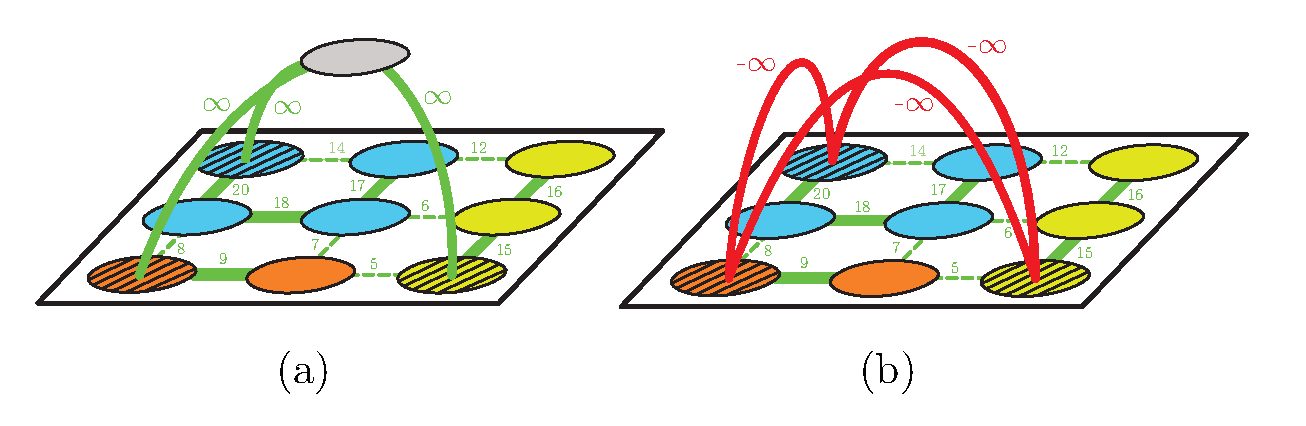
\includegraphics[width=\linewidth]{figures/MWS/images/seeded-WS.pdf}%
   %\includegraphics[width=0.8\linewidth]{egfigure.eps}
   \caption{Two equivalent representations of the seeded watershed clustering obtained using (a) a maximum spanning tree computation or (b) Algorithm \ref{WS_algo_code}. Both graphs share the weighted attractive~(green) edges and seeds (hatched nodes). The infinitely attractive connections to the auxiliary node (gray) in (a) are replaced by infinitely repulsive~(red) edges between each pair of seeds in (b). The two final clusterings are defined by the active sets (bold edges) and are identical. Node colors indicate the clustering result, but are arbitrary.}
\label{fig:WS_compare}
\end{figure}




\begin{algorithm}[t]
  \caption{Mutex version of seeded watershed algorithm}

  \begin{algorithmic}[1]
      \Procedure{SeededWatershed}{$\mathcal{G}(V,E),$ \text{\rm pos.\ weights} $w:E\rightarrow \mathbb  {R}^+$, \text{\rm seeds} $S\subseteq V$}
        \State $A^+ \leftarrow \emptyset$\; 
        \State $A^- \leftarrow \{ (s,t) \in S \times S \,|\, s \neq t \} $ % \Comment{Equiv. to adding infinitely repulsive edges between seeds}
        \For{$(i,j) = e \in E $ {\rm in descending order of } $w_e$} 
            \If{\rm {\bf not} $\operator{connected}$($i, j; A^+$) \textbf{and not} $\operator{mutex}$($i,j;A^+,A^-$) }  
                \State $A^+ \leftarrow A^+ \cup e$ \Comment{Merge $i,j$ and inherit mutex constraints of the parent clusters}
            \EndIf
        \EndFor
        \State
        \Return $A^+ \cup A^-$
      \EndProcedure
  \end{algorithmic}
    \algcomment{The output clustering is defined by the connected components of the final attractive active set $A^+$.}
 \label{WS_algo_code}
\end{algorithm}


\subsection{Seeded watershed from a mutex perspective}
\noindent One interpretation of the proposed method is in terms of a generalization of the edge-based watershed algorithm \cite{Meyer1994,Meyer1994minimum,meyer1999morphological}
 or image foresting transform \cite{falcao2004image}.
This algorithm can only ingest a graph with purely attractive interactions, $E^{-} = \emptyset$. Without  further constraints, the algorithm would yield only the trivial result of a single cluster comprising all vertices. To obtain more interesting output, an oracle needs to provide seeds~(e.g.\ one node per cluster). These seed vertices are all connected to an auxiliary node (see Fig.~\ref{fig:WS_compare} (a)) by auxiliary edges with infinite merge affinity. A maximum spanning tree (MST) on this augmented graph can be found in linearithmic time; and the maximum spanning tree (or in the case of degeneracy: at least one of the maximum spanning trees) will include the auxiliary edges. When the auxiliary edges are deleted from the MST, a forest results, with each tree representing one cluster \cite{meyer1999morphological,Meyer1994,falcao2004image}.

We now reformulate this well-known algorithm in a way that will later emerge as a special case of the proposed Mutex Watershed: 
we eliminate the auxiliary node and edges, and replace them by a set of infinitely repulsive edges, one for each pair of seeds (Fig.~\ref{fig:WS_compare} (b)).
Algorithm \ref{WS_algo_code} is a variation of Kruskal's MST algorithm operating on the seed mutex graph just defined, and gives results identical to seeded watershed on the original graph. 


This algorithm differs from Kruskal's only by the check for mutual exclusion in the if-statement. Obviously, the modified algorithm has the same effect as the original algorithm, because the final set $A^+$ is exactly the maximum spanning forest obtained after removing the auxiliary edges from the original solution. 

In the sequel, we generalize this construction by admitting less-than-infinitely repulsive edges. Importantly, these can be dense and are hence much easier to estimate automatically than seeds with their strict requirement of only-one-per-cluster.










\begin{algorithm}[t]
 % \hrulefill \\
  \caption{Mutex Watershed Algorithm}
  \begin{algorithmic}[1]
    \Procedure{MutexWatershed}{$\mathcal{G}(V,E)$, $w:E\rightarrow \mathbb{R}$, \text{\rm boolean $\operator{connect\_all}$}}
        \State $A^+ \leftarrow \emptyset; \quad A^- \leftarrow \emptyset $\;
        \For{$(i,j) = e \in E $ {\rm in descending order of } $|w_e|$} 
            \If{$e \in E^+$}
                \If{\rm \textbf{not} $\operator{mutex}$($i,j; A^+, A^-$) }  
                    \If{\rm {\bf not} $\operator{connected}$($i, j; A^+$) \textbf{or} \rm $\operator{connect\_all}$}
                        \State $\operator{merge}(i, j)$: $A^+ \leftarrow A^+ \cup e$
                        \Comment{Merge $i, j$ and inherit constraints of parent clusters}
                    \EndIf
                \EndIf
           \Else
                \If{\rm {\bf not} $\operator{connected}$($i, j; A^+$)}
                    \State $\operator{addmutex}(i, j)$: $A^- \leftarrow A^- \cup e$\;
                    \Comment{Add mutex constraint between $i$ and $j$}
                \EndIf
            \EndIf
        \EndFor
        \State 
        \Return $A^+ \cup A^-$
    \EndProcedure
    \end{algorithmic}
 \label{algo_code_efficient}
 \algcomment{\REVIEW{The output clustering is defined by the connected components of the final attractive active set $A^+$. The $\operator{connect\_all}$ parameter changes the internal cluster connectedness from trees to fully connected, but does not change the output clustering.} The $\operator{connected}$ predicate can be efficiently evaluated using union find data structures.}
% }
\end{algorithm}





\begin{figure}[htp]
\centering
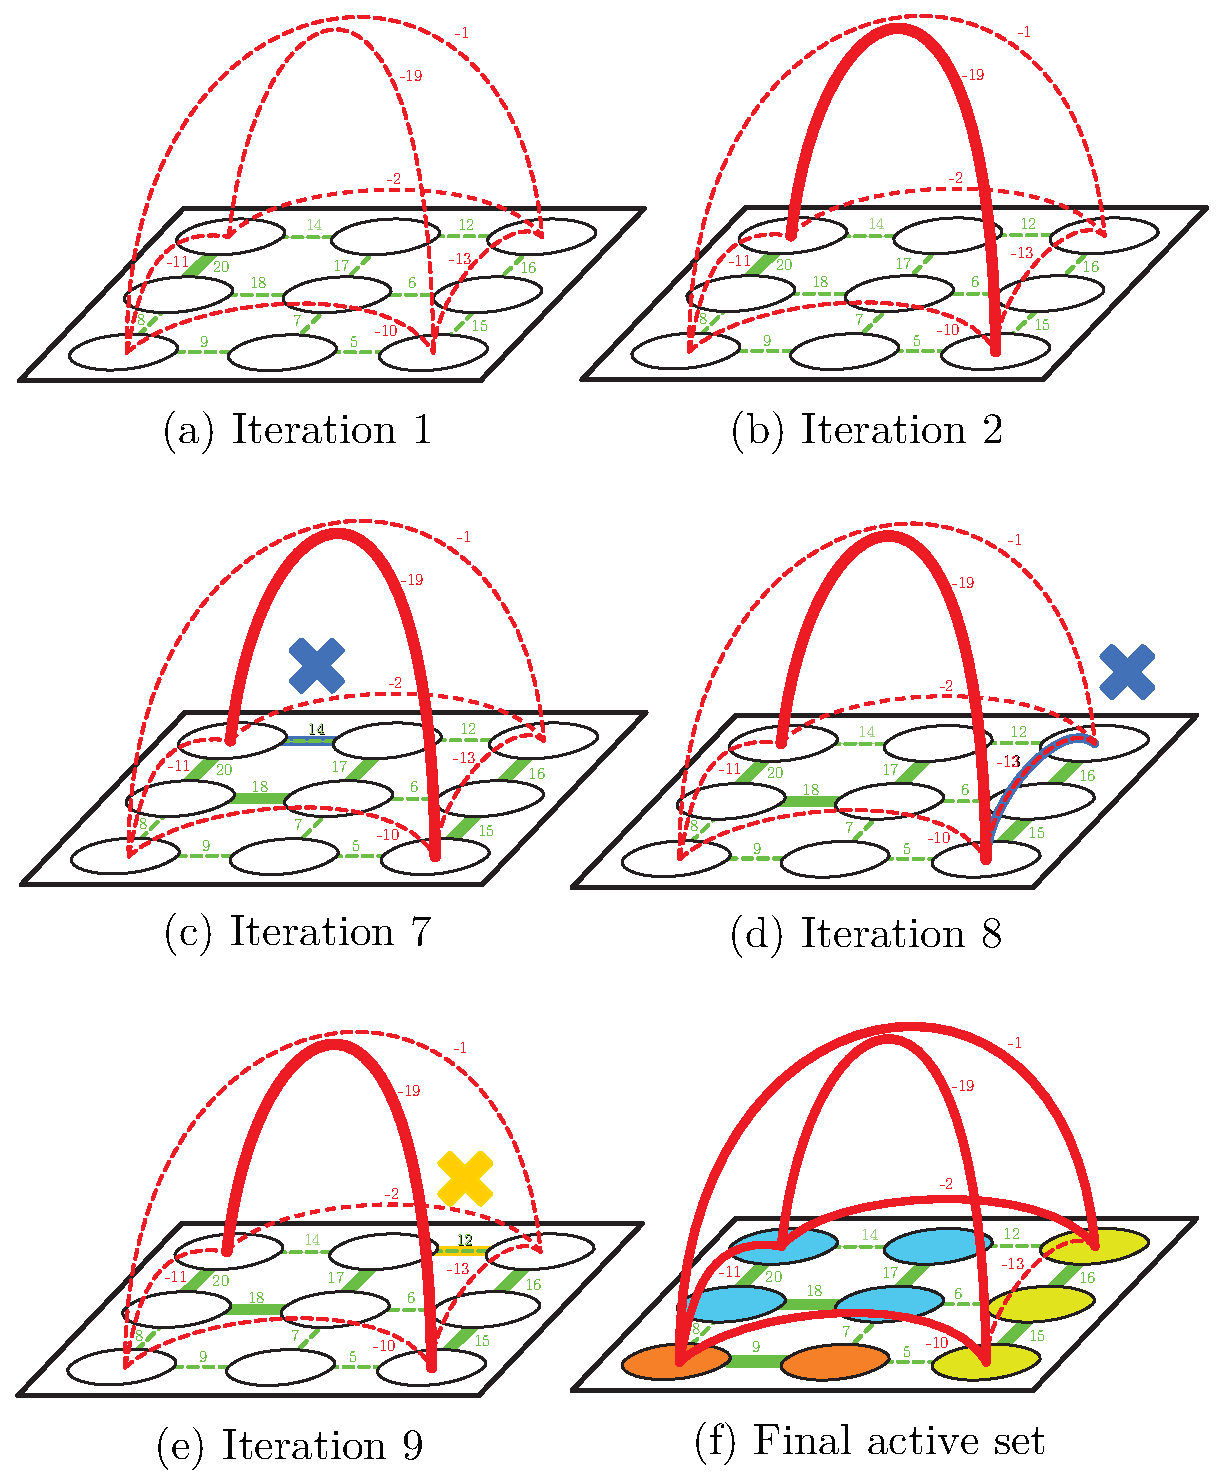
\includegraphics[width=0.9\linewidth]{figures/MWS/images/new-diagram-MWS-2.pdf}
% \includegraphics[width=\linewidth]{images/exampleg1.png}
% \includegraphics[width=\linewidth]{images/exampleg2.png}
   %\includegraphics[width=0.8\linewidth]{egfigure.eps}
   \caption{Some iterations of the Mutex Watershed Algorithm \ref{algo_code_efficient} applied to a graph with weighted attractive (green) and repulsive (red) edges. Edges accumulated in the active set $A$ after a given number of iterations are shown in bold. \REVIEW{The $\operator{connect\_all}$ parameter of the algorithm is set to $\operator{False}$, so that only the positive edges belonging to the maximum spanning tree of each cluster are added to the active set.} Once the algorithm terminates, the final active set (f) defines the final clustering (indicated using arbitrary node colors). Some edges are not added to the active set because they are mutex constrained~(yellow highlight) or because the associated nodes are already connected and in the same cluster~(blue highlight).}
   %Some edges that are not added to the active set because they would violate constraints $\mathcal{C}_{0}$ or $\mathcal{C}_{1}$ are highlighted in blue and yellow, respectively. \TODO{Update}}
\label{fig:MWS_algorithm}
\end{figure}

\subsection{Mutex Watersheds}\label{3_3_MWS}

\noindent 
We now introduce our core contribution: an algorithm that is empirically no more expensive than a MST computation; but that can ingest both attractive and repulsive cues and partition a graph into a number of clusters that does not need to be specified beforehand. \REVIEW{Neither seeds nor hyperparameters that implicitly determine the number of resulting clusters are required.}

The Mutex Watershed, Algorithm \ref{algo_code_efficient}, proceeds as follows. Given a graph $\mathcal{G}=(V, E)$ with signed weights $w: E \rightarrow \mathbb{R}$, do the following: sort all edges $E$, attractive or repulsive, by their absolute weight in descending order into a priority queue. Iteratively pop all edges from the queue and add them to the active set one by one, provided that a set of conditions are satisfied.
More specifically, assuming $\operator{connect\_all}$ is $\operator{False}$, if the next edge popped from the priority queue is attractive and its incident vertices are not yet in the same tree, then connect the respective trees provided this is not ruled out by a mutual exclusion constraint. If on the other hand the edge popped is repulsive, and if its incident vertices are not yet in the same tree, then add a mutual exclusion constraint between the two trees. 
The output clustering is defined by the connected components of the final attractive active set $A^+$.

 The crucial difference to Algorithm \ref{WS_algo_code} is that mutex constraints are no longer pre-defined, but created dynamically whenever a repulsive edge is found. However, new exclusion constraints can never override earlier, high-priority merge decisions. In this case, the repulsive edge in question is simply ignored. Similarly, an attractive edge must never override earlier and thus higher-priority must-not-link decisions. 

\REVIEW{The boolean value of the $\operator{connect\_all}$ input parameter of the algorithm does not influence the final output clustering, but defines the internal cluster connectedness: when it is set to $\operator{True}$, the algorithm adds all attractive intra-cluster edges to the active set $A^+$. When it is set to $\operator{False}$, then a maximum spanning tree is built for each cluster similarly to the seeded watershed. This variant of the algorithm will be helpful in the next section \ref{sec:MWS_objective} to highlight the relation between the Mutex Watershed and the multicut problem.}
% \TODO{Mention correctness, guaranteed termination?}

Fig. \ref{fig:MWS_algorithm} illustrates the proposed algorithm: Fig. \ref{fig:MWS_algorithm}a and Fig. \ref{fig:MWS_algorithm}b show examples of an unconstrained merge and an added mutex constraint, respectively; Fig. \ref{fig:MWS_algorithm}c and Fig. \ref{fig:MWS_algorithm}d show, respectively, an example of an attractive edge ($w_e=14$) and repulsive edge ($w_e=-13$) that are not added to the active set because their incident vertices  are already ``connected'' and belong to the same tree of the forest $A^+$; finally, Fig. \ref{fig:MWS_algorithm}e shows an attractive edge ($w_e=12$) that is ruled out by a previously introduced mutual exclusion relation.


\subsection{Time Complexity Analysis}


Before analyzing the time complexity of algorithm \ref{algo_code_efficient} we first review the complexity of Kruskal's algorithm. Using a union-find data structure~(with path compression and union by rank) the time complexity of $\operator{merge}(i,~j)$ and $\operator{connected}(i,~j)$ is $\mathcal{O}(\alpha(V))$, where $\alpha$ is the slowly growing inverse Ackerman function, and the total runtime complexity is dominated by the initial sorting of the edges $\mathcal{O}(E \log E)$\cite{cormen2009introduction}.

\noindent To check for mutex constraints efficiently, we maintain a set of all active mutex edges $$ M[C_i] = \{(u,~v) \in A^- | u \in C_i \lor v \in C_i\} $$ for every $C_i = \operator{cluster}(i)$ using hash tables, where insertion of new mutex edges~(i.e. $\operator{addmutex}$) and search have an average complexity of $\mathcal{O}(1)$. Note that every cluster can be efficiently identified by its union-find root node.
For $\operator{mutex}(i,~j)$ we check if $M[C_i] \cap M[C_j] = \emptyset$ by searching for all elements of the smaller hash table in the larger hash table. Therefore $\operator{mutex}(i,~j)$ has an average complexity of $\mathcal{O}(\min (|M[C_i]|, |M[C_j]|)$. % and a worst case complexity of $\mathcal{O}(|M[C_i]|\cdot|M[C_j]|)$.
Similarly, during $\operator{merge}(i,~j)$, mutex constraints are inherited  by merging two hash tables, which also has an average complexity $\mathcal{O}(\min (|M[C_i]|, |M[C_j]|)$. 

\noindent In conclusion, the average runtime contribution of attractive edges $\mathcal{O}(\max(|E^{+}| \cdot\alpha(V), |E^{+}| \cdot M))$ (checking mutex constraints and possibly merging) and repulsive edges
 $\mathcal{O}(\max(|E^{-}| \cdot \alpha(V), |E^{-}|)) $ (insertion of one mutex edge) result in a total average runtime complexity of algorithm \ref{algo_code_efficient}:
 \vspace{-0.1cm}
    % \begin{equation}
    %     \mathcal{O}(E \log E + E  \cdot  \alpha(V) + EM).
    % \end{equation}
    \begin{equation}
         \mathcal{O}(\max(E \log E \;,\; EM)).
    \end{equation}
where $M$ is the expected value of $\min (|M[C_i]|, |M[C_j]|)$ and $\alpha(V) \in \mathcal{O}(\log V) \in \mathcal{O}(\log E) $ \footnote{In the worst case $G$ is a fully connected graph, with $|E|=|V|^2$, hence $\log |V| = \frac{1}{2} \log |E|$.}.


\noindent In the worst case $\mathcal{O}(M) \in \mathcal{O}(E)$, the Mutex Watershed Algorithm has a runtime complexity of  $\mathcal{O}(E^2)$. Empirically, we find that $\mathcal{O}(EM) \approx \mathcal{O}(E\log E)$ by measuring the runtime of Mutex Watershed for different sub-volumes of the ISBI challenge~(see Figure \ref{fig:scalingM}), leading to a 
\begin{equation}
    \text{Empirical Mutex Watershed Complexity: }\mathcal{O}(E \log E)
\end{equation}


\begin{figure}[ht]
   \centering
\adjustbox{width=0.88\linewidth}{
       %% Creator: Matplotlib, PGF backend
%%
%% To include the figure in your LaTeX document, write
%%   \input{<filename>.pgf}
%%
%% Make sure the required packages are loaded in your preamble
%%   \usepackage{pgf}
%%
%% Figures using additional raster images can only be included by \input if
%% they are in the same directory as the main LaTeX file. For loading figures
%% from other directories you can use the `import` package
%%   \usepackage{import}
%% and then include the figures with
%%   \import{<path to file>}{<filename>.pgf}
%%
%% Matplotlib used the following preamble
%%   \usepackage{fontspec}
%%   \setmainfont{DejaVu Serif}
%%   \setsansfont{DejaVu Sans}
%%   \setmonofont{DejaVu Sans Mono}
%%
\begingroup%
\makeatletter%
\begin{pgfpicture}%
\pgfpathrectangle{\pgfpointorigin}{\pgfqpoint{7.000000in}{7.000000in}}%
\pgfusepath{use as bounding box, clip}%
\begin{pgfscope}%
\pgfsetbuttcap%
\pgfsetmiterjoin%
\definecolor{currentfill}{rgb}{1.000000,1.000000,1.000000}%
\pgfsetfillcolor{currentfill}%
\pgfsetlinewidth{0.000000pt}%
\definecolor{currentstroke}{rgb}{1.000000,1.000000,1.000000}%
\pgfsetstrokecolor{currentstroke}%
\pgfsetdash{}{0pt}%
\pgfpathmoveto{\pgfqpoint{0.000000in}{0.000000in}}%
\pgfpathlineto{\pgfqpoint{7.000000in}{0.000000in}}%
\pgfpathlineto{\pgfqpoint{7.000000in}{7.000000in}}%
\pgfpathlineto{\pgfqpoint{0.000000in}{7.000000in}}%
\pgfpathclose%
\pgfusepath{fill}%
\end{pgfscope}%
\begin{pgfscope}%
\pgfsetbuttcap%
\pgfsetmiterjoin%
\definecolor{currentfill}{rgb}{0.917647,0.917647,0.949020}%
\pgfsetfillcolor{currentfill}%
\pgfsetlinewidth{0.000000pt}%
\definecolor{currentstroke}{rgb}{0.000000,0.000000,0.000000}%
\pgfsetstrokecolor{currentstroke}%
\pgfsetstrokeopacity{0.000000}%
\pgfsetdash{}{0pt}%
\pgfpathmoveto{\pgfqpoint{0.875000in}{0.770000in}}%
\pgfpathlineto{\pgfqpoint{6.300000in}{0.770000in}}%
\pgfpathlineto{\pgfqpoint{6.300000in}{6.160000in}}%
\pgfpathlineto{\pgfqpoint{0.875000in}{6.160000in}}%
\pgfpathclose%
\pgfusepath{fill}%
\end{pgfscope}%
\begin{pgfscope}%
\pgfpathrectangle{\pgfqpoint{0.875000in}{0.770000in}}{\pgfqpoint{5.425000in}{5.390000in}}%
\pgfusepath{clip}%
\pgfsetroundcap%
\pgfsetroundjoin%
\pgfsetlinewidth{1.003750pt}%
\definecolor{currentstroke}{rgb}{1.000000,1.000000,1.000000}%
\pgfsetstrokecolor{currentstroke}%
\pgfsetdash{}{0pt}%
\pgfpathmoveto{\pgfqpoint{1.125582in}{0.770000in}}%
\pgfpathlineto{\pgfqpoint{1.125582in}{6.160000in}}%
\pgfusepath{stroke}%
\end{pgfscope}%
\begin{pgfscope}%
\definecolor{textcolor}{rgb}{0.150000,0.150000,0.150000}%
\pgfsetstrokecolor{textcolor}%
\pgfsetfillcolor{textcolor}%
\pgftext[x=1.125582in,y=0.638056in,,top]{\color{textcolor}\sffamily\fontsize{11.000000}{13.200000}\selectfont \(\displaystyle 10^{6}\)}%
\end{pgfscope}%
\begin{pgfscope}%
\pgfpathrectangle{\pgfqpoint{0.875000in}{0.770000in}}{\pgfqpoint{5.425000in}{5.390000in}}%
\pgfusepath{clip}%
\pgfsetroundcap%
\pgfsetroundjoin%
\pgfsetlinewidth{1.003750pt}%
\definecolor{currentstroke}{rgb}{1.000000,1.000000,1.000000}%
\pgfsetstrokecolor{currentstroke}%
\pgfsetdash{}{0pt}%
\pgfpathmoveto{\pgfqpoint{4.010989in}{0.770000in}}%
\pgfpathlineto{\pgfqpoint{4.010989in}{6.160000in}}%
\pgfusepath{stroke}%
\end{pgfscope}%
\begin{pgfscope}%
\definecolor{textcolor}{rgb}{0.150000,0.150000,0.150000}%
\pgfsetstrokecolor{textcolor}%
\pgfsetfillcolor{textcolor}%
\pgftext[x=4.010989in,y=0.638056in,,top]{\color{textcolor}\sffamily\fontsize{11.000000}{13.200000}\selectfont \(\displaystyle 10^{7}\)}%
\end{pgfscope}%
\begin{pgfscope}%
\definecolor{textcolor}{rgb}{0.150000,0.150000,0.150000}%
\pgfsetstrokecolor{textcolor}%
\pgfsetfillcolor{textcolor}%
\pgftext[x=3.587500in,y=0.434646in,,top]{\color{textcolor}\sffamily\fontsize{12.000000}{14.400000}\selectfont Total Number of Edges |E|}%
\end{pgfscope}%
\begin{pgfscope}%
\pgfpathrectangle{\pgfqpoint{0.875000in}{0.770000in}}{\pgfqpoint{5.425000in}{5.390000in}}%
\pgfusepath{clip}%
\pgfsetroundcap%
\pgfsetroundjoin%
\pgfsetlinewidth{1.003750pt}%
\definecolor{currentstroke}{rgb}{1.000000,1.000000,1.000000}%
\pgfsetstrokecolor{currentstroke}%
\pgfsetdash{}{0pt}%
\pgfpathmoveto{\pgfqpoint{0.875000in}{0.950170in}}%
\pgfpathlineto{\pgfqpoint{6.300000in}{0.950170in}}%
\pgfusepath{stroke}%
\end{pgfscope}%
\begin{pgfscope}%
\definecolor{textcolor}{rgb}{0.150000,0.150000,0.150000}%
\pgfsetstrokecolor{textcolor}%
\pgfsetfillcolor{textcolor}%
\pgftext[x=0.500088in,y=0.892132in,left,base]{\color{textcolor}\sffamily\fontsize{11.000000}{13.200000}\selectfont 0.5}%
\end{pgfscope}%
\begin{pgfscope}%
\pgfpathrectangle{\pgfqpoint{0.875000in}{0.770000in}}{\pgfqpoint{5.425000in}{5.390000in}}%
\pgfusepath{clip}%
\pgfsetroundcap%
\pgfsetroundjoin%
\pgfsetlinewidth{1.003750pt}%
\definecolor{currentstroke}{rgb}{1.000000,1.000000,1.000000}%
\pgfsetstrokecolor{currentstroke}%
\pgfsetdash{}{0pt}%
\pgfpathmoveto{\pgfqpoint{0.875000in}{1.742783in}}%
\pgfpathlineto{\pgfqpoint{6.300000in}{1.742783in}}%
\pgfusepath{stroke}%
\end{pgfscope}%
\begin{pgfscope}%
\definecolor{textcolor}{rgb}{0.150000,0.150000,0.150000}%
\pgfsetstrokecolor{textcolor}%
\pgfsetfillcolor{textcolor}%
\pgftext[x=0.500088in,y=1.684746in,left,base]{\color{textcolor}\sffamily\fontsize{11.000000}{13.200000}\selectfont 1.0}%
\end{pgfscope}%
\begin{pgfscope}%
\pgfpathrectangle{\pgfqpoint{0.875000in}{0.770000in}}{\pgfqpoint{5.425000in}{5.390000in}}%
\pgfusepath{clip}%
\pgfsetroundcap%
\pgfsetroundjoin%
\pgfsetlinewidth{1.003750pt}%
\definecolor{currentstroke}{rgb}{1.000000,1.000000,1.000000}%
\pgfsetstrokecolor{currentstroke}%
\pgfsetdash{}{0pt}%
\pgfpathmoveto{\pgfqpoint{0.875000in}{2.535397in}}%
\pgfpathlineto{\pgfqpoint{6.300000in}{2.535397in}}%
\pgfusepath{stroke}%
\end{pgfscope}%
\begin{pgfscope}%
\definecolor{textcolor}{rgb}{0.150000,0.150000,0.150000}%
\pgfsetstrokecolor{textcolor}%
\pgfsetfillcolor{textcolor}%
\pgftext[x=0.500088in,y=2.477360in,left,base]{\color{textcolor}\sffamily\fontsize{11.000000}{13.200000}\selectfont 1.5}%
\end{pgfscope}%
\begin{pgfscope}%
\pgfpathrectangle{\pgfqpoint{0.875000in}{0.770000in}}{\pgfqpoint{5.425000in}{5.390000in}}%
\pgfusepath{clip}%
\pgfsetroundcap%
\pgfsetroundjoin%
\pgfsetlinewidth{1.003750pt}%
\definecolor{currentstroke}{rgb}{1.000000,1.000000,1.000000}%
\pgfsetstrokecolor{currentstroke}%
\pgfsetdash{}{0pt}%
\pgfpathmoveto{\pgfqpoint{0.875000in}{3.328011in}}%
\pgfpathlineto{\pgfqpoint{6.300000in}{3.328011in}}%
\pgfusepath{stroke}%
\end{pgfscope}%
\begin{pgfscope}%
\definecolor{textcolor}{rgb}{0.150000,0.150000,0.150000}%
\pgfsetstrokecolor{textcolor}%
\pgfsetfillcolor{textcolor}%
\pgftext[x=0.500088in,y=3.269973in,left,base]{\color{textcolor}\sffamily\fontsize{11.000000}{13.200000}\selectfont 2.0}%
\end{pgfscope}%
\begin{pgfscope}%
\pgfpathrectangle{\pgfqpoint{0.875000in}{0.770000in}}{\pgfqpoint{5.425000in}{5.390000in}}%
\pgfusepath{clip}%
\pgfsetroundcap%
\pgfsetroundjoin%
\pgfsetlinewidth{1.003750pt}%
\definecolor{currentstroke}{rgb}{1.000000,1.000000,1.000000}%
\pgfsetstrokecolor{currentstroke}%
\pgfsetdash{}{0pt}%
\pgfpathmoveto{\pgfqpoint{0.875000in}{4.120625in}}%
\pgfpathlineto{\pgfqpoint{6.300000in}{4.120625in}}%
\pgfusepath{stroke}%
\end{pgfscope}%
\begin{pgfscope}%
\definecolor{textcolor}{rgb}{0.150000,0.150000,0.150000}%
\pgfsetstrokecolor{textcolor}%
\pgfsetfillcolor{textcolor}%
\pgftext[x=0.500088in,y=4.062587in,left,base]{\color{textcolor}\sffamily\fontsize{11.000000}{13.200000}\selectfont 2.5}%
\end{pgfscope}%
\begin{pgfscope}%
\pgfpathrectangle{\pgfqpoint{0.875000in}{0.770000in}}{\pgfqpoint{5.425000in}{5.390000in}}%
\pgfusepath{clip}%
\pgfsetroundcap%
\pgfsetroundjoin%
\pgfsetlinewidth{1.003750pt}%
\definecolor{currentstroke}{rgb}{1.000000,1.000000,1.000000}%
\pgfsetstrokecolor{currentstroke}%
\pgfsetdash{}{0pt}%
\pgfpathmoveto{\pgfqpoint{0.875000in}{4.913239in}}%
\pgfpathlineto{\pgfqpoint{6.300000in}{4.913239in}}%
\pgfusepath{stroke}%
\end{pgfscope}%
\begin{pgfscope}%
\definecolor{textcolor}{rgb}{0.150000,0.150000,0.150000}%
\pgfsetstrokecolor{textcolor}%
\pgfsetfillcolor{textcolor}%
\pgftext[x=0.500088in,y=4.855201in,left,base]{\color{textcolor}\sffamily\fontsize{11.000000}{13.200000}\selectfont 3.0}%
\end{pgfscope}%
\begin{pgfscope}%
\pgfpathrectangle{\pgfqpoint{0.875000in}{0.770000in}}{\pgfqpoint{5.425000in}{5.390000in}}%
\pgfusepath{clip}%
\pgfsetroundcap%
\pgfsetroundjoin%
\pgfsetlinewidth{1.003750pt}%
\definecolor{currentstroke}{rgb}{1.000000,1.000000,1.000000}%
\pgfsetstrokecolor{currentstroke}%
\pgfsetdash{}{0pt}%
\pgfpathmoveto{\pgfqpoint{0.875000in}{5.705853in}}%
\pgfpathlineto{\pgfqpoint{6.300000in}{5.705853in}}%
\pgfusepath{stroke}%
\end{pgfscope}%
\begin{pgfscope}%
\definecolor{textcolor}{rgb}{0.150000,0.150000,0.150000}%
\pgfsetstrokecolor{textcolor}%
\pgfsetfillcolor{textcolor}%
\pgftext[x=0.500088in,y=5.647815in,left,base]{\color{textcolor}\sffamily\fontsize{11.000000}{13.200000}\selectfont 3.5}%
\end{pgfscope}%
\begin{pgfscope}%
\definecolor{textcolor}{rgb}{0.150000,0.150000,0.150000}%
\pgfsetstrokecolor{textcolor}%
\pgfsetfillcolor{textcolor}%
\pgftext[x=0.444533in,y=3.465000in,,bottom,rotate=90.000000]{\color{textcolor}\sffamily\fontsize{12.000000}{14.400000}\selectfont Runtime[s] / Total Number of Edges |E|}%
\end{pgfscope}%
\begin{pgfscope}%
\definecolor{textcolor}{rgb}{0.150000,0.150000,0.150000}%
\pgfsetstrokecolor{textcolor}%
\pgfsetfillcolor{textcolor}%
\pgftext[x=0.875000in,y=6.201667in,left,base]{\color{textcolor}\sffamily\fontsize{11.000000}{13.200000}\selectfont 1e-7}%
\end{pgfscope}%
\begin{pgfscope}%
\pgfpathrectangle{\pgfqpoint{0.875000in}{0.770000in}}{\pgfqpoint{5.425000in}{5.390000in}}%
\pgfusepath{clip}%
\pgfsetbuttcap%
\pgfsetroundjoin%
\definecolor{currentfill}{rgb}{0.298039,0.447059,0.690196}%
\pgfsetfillcolor{currentfill}%
\pgfsetfillopacity{0.800000}%
\pgfsetlinewidth{1.003750pt}%
\definecolor{currentstroke}{rgb}{0.298039,0.447059,0.690196}%
\pgfsetstrokecolor{currentstroke}%
\pgfsetstrokeopacity{0.800000}%
\pgfsetdash{}{0pt}%
\pgfpathmoveto{\pgfqpoint{1.139143in}{1.833385in}}%
\pgfpathcurveto{\pgfqpoint{1.150193in}{1.833385in}}{\pgfqpoint{1.160792in}{1.837775in}}{\pgfqpoint{1.168605in}{1.845589in}}%
\pgfpathcurveto{\pgfqpoint{1.176419in}{1.853402in}}{\pgfqpoint{1.180809in}{1.864002in}}{\pgfqpoint{1.180809in}{1.875052in}}%
\pgfpathcurveto{\pgfqpoint{1.180809in}{1.886102in}}{\pgfqpoint{1.176419in}{1.896701in}}{\pgfqpoint{1.168605in}{1.904514in}}%
\pgfpathcurveto{\pgfqpoint{1.160792in}{1.912328in}}{\pgfqpoint{1.150193in}{1.916718in}}{\pgfqpoint{1.139143in}{1.916718in}}%
\pgfpathcurveto{\pgfqpoint{1.128093in}{1.916718in}}{\pgfqpoint{1.117494in}{1.912328in}}{\pgfqpoint{1.109680in}{1.904514in}}%
\pgfpathcurveto{\pgfqpoint{1.101866in}{1.896701in}}{\pgfqpoint{1.097476in}{1.886102in}}{\pgfqpoint{1.097476in}{1.875052in}}%
\pgfpathcurveto{\pgfqpoint{1.097476in}{1.864002in}}{\pgfqpoint{1.101866in}{1.853402in}}{\pgfqpoint{1.109680in}{1.845589in}}%
\pgfpathcurveto{\pgfqpoint{1.117494in}{1.837775in}}{\pgfqpoint{1.128093in}{1.833385in}}{\pgfqpoint{1.139143in}{1.833385in}}%
\pgfpathclose%
\pgfusepath{stroke,fill}%
\end{pgfscope}%
\begin{pgfscope}%
\pgfpathrectangle{\pgfqpoint{0.875000in}{0.770000in}}{\pgfqpoint{5.425000in}{5.390000in}}%
\pgfusepath{clip}%
\pgfsetbuttcap%
\pgfsetroundjoin%
\definecolor{currentfill}{rgb}{0.298039,0.447059,0.690196}%
\pgfsetfillcolor{currentfill}%
\pgfsetfillopacity{0.800000}%
\pgfsetlinewidth{1.003750pt}%
\definecolor{currentstroke}{rgb}{0.298039,0.447059,0.690196}%
\pgfsetstrokecolor{currentstroke}%
\pgfsetstrokeopacity{0.800000}%
\pgfsetdash{}{0pt}%
\pgfpathmoveto{\pgfqpoint{1.274648in}{1.812083in}}%
\pgfpathcurveto{\pgfqpoint{1.285698in}{1.812083in}}{\pgfqpoint{1.296297in}{1.816473in}}{\pgfqpoint{1.304110in}{1.824287in}}%
\pgfpathcurveto{\pgfqpoint{1.311924in}{1.832100in}}{\pgfqpoint{1.316314in}{1.842699in}}{\pgfqpoint{1.316314in}{1.853749in}}%
\pgfpathcurveto{\pgfqpoint{1.316314in}{1.864799in}}{\pgfqpoint{1.311924in}{1.875399in}}{\pgfqpoint{1.304110in}{1.883212in}}%
\pgfpathcurveto{\pgfqpoint{1.296297in}{1.891026in}}{\pgfqpoint{1.285698in}{1.895416in}}{\pgfqpoint{1.274648in}{1.895416in}}%
\pgfpathcurveto{\pgfqpoint{1.263598in}{1.895416in}}{\pgfqpoint{1.252999in}{1.891026in}}{\pgfqpoint{1.245185in}{1.883212in}}%
\pgfpathcurveto{\pgfqpoint{1.237371in}{1.875399in}}{\pgfqpoint{1.232981in}{1.864799in}}{\pgfqpoint{1.232981in}{1.853749in}}%
\pgfpathcurveto{\pgfqpoint{1.232981in}{1.842699in}}{\pgfqpoint{1.237371in}{1.832100in}}{\pgfqpoint{1.245185in}{1.824287in}}%
\pgfpathcurveto{\pgfqpoint{1.252999in}{1.816473in}}{\pgfqpoint{1.263598in}{1.812083in}}{\pgfqpoint{1.274648in}{1.812083in}}%
\pgfpathclose%
\pgfusepath{stroke,fill}%
\end{pgfscope}%
\begin{pgfscope}%
\pgfpathrectangle{\pgfqpoint{0.875000in}{0.770000in}}{\pgfqpoint{5.425000in}{5.390000in}}%
\pgfusepath{clip}%
\pgfsetbuttcap%
\pgfsetroundjoin%
\definecolor{currentfill}{rgb}{0.298039,0.447059,0.690196}%
\pgfsetfillcolor{currentfill}%
\pgfsetfillopacity{0.800000}%
\pgfsetlinewidth{1.003750pt}%
\definecolor{currentstroke}{rgb}{0.298039,0.447059,0.690196}%
\pgfsetstrokecolor{currentstroke}%
\pgfsetstrokeopacity{0.800000}%
\pgfsetdash{}{0pt}%
\pgfpathmoveto{\pgfqpoint{1.403201in}{1.894457in}}%
\pgfpathcurveto{\pgfqpoint{1.414251in}{1.894457in}}{\pgfqpoint{1.424850in}{1.898847in}}{\pgfqpoint{1.432663in}{1.906661in}}%
\pgfpathcurveto{\pgfqpoint{1.440477in}{1.914475in}}{\pgfqpoint{1.444867in}{1.925074in}}{\pgfqpoint{1.444867in}{1.936124in}}%
\pgfpathcurveto{\pgfqpoint{1.444867in}{1.947174in}}{\pgfqpoint{1.440477in}{1.957773in}}{\pgfqpoint{1.432663in}{1.965587in}}%
\pgfpathcurveto{\pgfqpoint{1.424850in}{1.973400in}}{\pgfqpoint{1.414251in}{1.977791in}}{\pgfqpoint{1.403201in}{1.977791in}}%
\pgfpathcurveto{\pgfqpoint{1.392150in}{1.977791in}}{\pgfqpoint{1.381551in}{1.973400in}}{\pgfqpoint{1.373738in}{1.965587in}}%
\pgfpathcurveto{\pgfqpoint{1.365924in}{1.957773in}}{\pgfqpoint{1.361534in}{1.947174in}}{\pgfqpoint{1.361534in}{1.936124in}}%
\pgfpathcurveto{\pgfqpoint{1.361534in}{1.925074in}}{\pgfqpoint{1.365924in}{1.914475in}}{\pgfqpoint{1.373738in}{1.906661in}}%
\pgfpathcurveto{\pgfqpoint{1.381551in}{1.898847in}}{\pgfqpoint{1.392150in}{1.894457in}}{\pgfqpoint{1.403201in}{1.894457in}}%
\pgfpathclose%
\pgfusepath{stroke,fill}%
\end{pgfscope}%
\begin{pgfscope}%
\pgfpathrectangle{\pgfqpoint{0.875000in}{0.770000in}}{\pgfqpoint{5.425000in}{5.390000in}}%
\pgfusepath{clip}%
\pgfsetbuttcap%
\pgfsetroundjoin%
\definecolor{currentfill}{rgb}{0.298039,0.447059,0.690196}%
\pgfsetfillcolor{currentfill}%
\pgfsetfillopacity{0.800000}%
\pgfsetlinewidth{1.003750pt}%
\definecolor{currentstroke}{rgb}{0.298039,0.447059,0.690196}%
\pgfsetstrokecolor{currentstroke}%
\pgfsetstrokeopacity{0.800000}%
\pgfsetdash{}{0pt}%
\pgfpathmoveto{\pgfqpoint{1.525480in}{2.049867in}}%
\pgfpathcurveto{\pgfqpoint{1.536530in}{2.049867in}}{\pgfqpoint{1.547129in}{2.054257in}}{\pgfqpoint{1.554943in}{2.062071in}}%
\pgfpathcurveto{\pgfqpoint{1.562756in}{2.069884in}}{\pgfqpoint{1.567147in}{2.080483in}}{\pgfqpoint{1.567147in}{2.091533in}}%
\pgfpathcurveto{\pgfqpoint{1.567147in}{2.102584in}}{\pgfqpoint{1.562756in}{2.113183in}}{\pgfqpoint{1.554943in}{2.120996in}}%
\pgfpathcurveto{\pgfqpoint{1.547129in}{2.128810in}}{\pgfqpoint{1.536530in}{2.133200in}}{\pgfqpoint{1.525480in}{2.133200in}}%
\pgfpathcurveto{\pgfqpoint{1.514430in}{2.133200in}}{\pgfqpoint{1.503831in}{2.128810in}}{\pgfqpoint{1.496017in}{2.120996in}}%
\pgfpathcurveto{\pgfqpoint{1.488204in}{2.113183in}}{\pgfqpoint{1.483813in}{2.102584in}}{\pgfqpoint{1.483813in}{2.091533in}}%
\pgfpathcurveto{\pgfqpoint{1.483813in}{2.080483in}}{\pgfqpoint{1.488204in}{2.069884in}}{\pgfqpoint{1.496017in}{2.062071in}}%
\pgfpathcurveto{\pgfqpoint{1.503831in}{2.054257in}}{\pgfqpoint{1.514430in}{2.049867in}}{\pgfqpoint{1.525480in}{2.049867in}}%
\pgfpathclose%
\pgfusepath{stroke,fill}%
\end{pgfscope}%
\begin{pgfscope}%
\pgfpathrectangle{\pgfqpoint{0.875000in}{0.770000in}}{\pgfqpoint{5.425000in}{5.390000in}}%
\pgfusepath{clip}%
\pgfsetbuttcap%
\pgfsetroundjoin%
\definecolor{currentfill}{rgb}{0.298039,0.447059,0.690196}%
\pgfsetfillcolor{currentfill}%
\pgfsetfillopacity{0.800000}%
\pgfsetlinewidth{1.003750pt}%
\definecolor{currentstroke}{rgb}{0.298039,0.447059,0.690196}%
\pgfsetstrokecolor{currentstroke}%
\pgfsetstrokeopacity{0.800000}%
\pgfsetdash{}{0pt}%
\pgfpathmoveto{\pgfqpoint{1.642070in}{1.914527in}}%
\pgfpathcurveto{\pgfqpoint{1.653120in}{1.914527in}}{\pgfqpoint{1.663719in}{1.918917in}}{\pgfqpoint{1.671533in}{1.926731in}}%
\pgfpathcurveto{\pgfqpoint{1.679346in}{1.934545in}}{\pgfqpoint{1.683737in}{1.945144in}}{\pgfqpoint{1.683737in}{1.956194in}}%
\pgfpathcurveto{\pgfqpoint{1.683737in}{1.967244in}}{\pgfqpoint{1.679346in}{1.977843in}}{\pgfqpoint{1.671533in}{1.985657in}}%
\pgfpathcurveto{\pgfqpoint{1.663719in}{1.993470in}}{\pgfqpoint{1.653120in}{1.997860in}}{\pgfqpoint{1.642070in}{1.997860in}}%
\pgfpathcurveto{\pgfqpoint{1.631020in}{1.997860in}}{\pgfqpoint{1.620421in}{1.993470in}}{\pgfqpoint{1.612607in}{1.985657in}}%
\pgfpathcurveto{\pgfqpoint{1.604794in}{1.977843in}}{\pgfqpoint{1.600403in}{1.967244in}}{\pgfqpoint{1.600403in}{1.956194in}}%
\pgfpathcurveto{\pgfqpoint{1.600403in}{1.945144in}}{\pgfqpoint{1.604794in}{1.934545in}}{\pgfqpoint{1.612607in}{1.926731in}}%
\pgfpathcurveto{\pgfqpoint{1.620421in}{1.918917in}}{\pgfqpoint{1.631020in}{1.914527in}}{\pgfqpoint{1.642070in}{1.914527in}}%
\pgfpathclose%
\pgfusepath{stroke,fill}%
\end{pgfscope}%
\begin{pgfscope}%
\pgfpathrectangle{\pgfqpoint{0.875000in}{0.770000in}}{\pgfqpoint{5.425000in}{5.390000in}}%
\pgfusepath{clip}%
\pgfsetbuttcap%
\pgfsetroundjoin%
\definecolor{currentfill}{rgb}{0.298039,0.447059,0.690196}%
\pgfsetfillcolor{currentfill}%
\pgfsetfillopacity{0.800000}%
\pgfsetlinewidth{1.003750pt}%
\definecolor{currentstroke}{rgb}{0.298039,0.447059,0.690196}%
\pgfsetstrokecolor{currentstroke}%
\pgfsetstrokeopacity{0.800000}%
\pgfsetdash{}{0pt}%
\pgfpathmoveto{\pgfqpoint{1.753476in}{1.925091in}}%
\pgfpathcurveto{\pgfqpoint{1.764527in}{1.925091in}}{\pgfqpoint{1.775126in}{1.929481in}}{\pgfqpoint{1.782939in}{1.937295in}}%
\pgfpathcurveto{\pgfqpoint{1.790753in}{1.945109in}}{\pgfqpoint{1.795143in}{1.955708in}}{\pgfqpoint{1.795143in}{1.966758in}}%
\pgfpathcurveto{\pgfqpoint{1.795143in}{1.977808in}}{\pgfqpoint{1.790753in}{1.988407in}}{\pgfqpoint{1.782939in}{1.996220in}}%
\pgfpathcurveto{\pgfqpoint{1.775126in}{2.004034in}}{\pgfqpoint{1.764527in}{2.008424in}}{\pgfqpoint{1.753476in}{2.008424in}}%
\pgfpathcurveto{\pgfqpoint{1.742426in}{2.008424in}}{\pgfqpoint{1.731827in}{2.004034in}}{\pgfqpoint{1.724014in}{1.996220in}}%
\pgfpathcurveto{\pgfqpoint{1.716200in}{1.988407in}}{\pgfqpoint{1.711810in}{1.977808in}}{\pgfqpoint{1.711810in}{1.966758in}}%
\pgfpathcurveto{\pgfqpoint{1.711810in}{1.955708in}}{\pgfqpoint{1.716200in}{1.945109in}}{\pgfqpoint{1.724014in}{1.937295in}}%
\pgfpathcurveto{\pgfqpoint{1.731827in}{1.929481in}}{\pgfqpoint{1.742426in}{1.925091in}}{\pgfqpoint{1.753476in}{1.925091in}}%
\pgfpathclose%
\pgfusepath{stroke,fill}%
\end{pgfscope}%
\begin{pgfscope}%
\pgfpathrectangle{\pgfqpoint{0.875000in}{0.770000in}}{\pgfqpoint{5.425000in}{5.390000in}}%
\pgfusepath{clip}%
\pgfsetbuttcap%
\pgfsetroundjoin%
\definecolor{currentfill}{rgb}{0.298039,0.447059,0.690196}%
\pgfsetfillcolor{currentfill}%
\pgfsetfillopacity{0.800000}%
\pgfsetlinewidth{1.003750pt}%
\definecolor{currentstroke}{rgb}{0.298039,0.447059,0.690196}%
\pgfsetstrokecolor{currentstroke}%
\pgfsetstrokeopacity{0.800000}%
\pgfsetdash{}{0pt}%
\pgfpathmoveto{\pgfqpoint{1.860141in}{2.049867in}}%
\pgfpathcurveto{\pgfqpoint{1.871191in}{2.049867in}}{\pgfqpoint{1.881790in}{2.054257in}}{\pgfqpoint{1.889604in}{2.062071in}}%
\pgfpathcurveto{\pgfqpoint{1.897417in}{2.069884in}}{\pgfqpoint{1.901807in}{2.080483in}}{\pgfqpoint{1.901807in}{2.091533in}}%
\pgfpathcurveto{\pgfqpoint{1.901807in}{2.102584in}}{\pgfqpoint{1.897417in}{2.113183in}}{\pgfqpoint{1.889604in}{2.120996in}}%
\pgfpathcurveto{\pgfqpoint{1.881790in}{2.128810in}}{\pgfqpoint{1.871191in}{2.133200in}}{\pgfqpoint{1.860141in}{2.133200in}}%
\pgfpathcurveto{\pgfqpoint{1.849091in}{2.133200in}}{\pgfqpoint{1.838492in}{2.128810in}}{\pgfqpoint{1.830678in}{2.120996in}}%
\pgfpathcurveto{\pgfqpoint{1.822864in}{2.113183in}}{\pgfqpoint{1.818474in}{2.102584in}}{\pgfqpoint{1.818474in}{2.091533in}}%
\pgfpathcurveto{\pgfqpoint{1.818474in}{2.080483in}}{\pgfqpoint{1.822864in}{2.069884in}}{\pgfqpoint{1.830678in}{2.062071in}}%
\pgfpathcurveto{\pgfqpoint{1.838492in}{2.054257in}}{\pgfqpoint{1.849091in}{2.049867in}}{\pgfqpoint{1.860141in}{2.049867in}}%
\pgfpathclose%
\pgfusepath{stroke,fill}%
\end{pgfscope}%
\begin{pgfscope}%
\pgfpathrectangle{\pgfqpoint{0.875000in}{0.770000in}}{\pgfqpoint{5.425000in}{5.390000in}}%
\pgfusepath{clip}%
\pgfsetbuttcap%
\pgfsetroundjoin%
\definecolor{currentfill}{rgb}{0.298039,0.447059,0.690196}%
\pgfsetfillcolor{currentfill}%
\pgfsetfillopacity{0.800000}%
\pgfsetlinewidth{1.003750pt}%
\definecolor{currentstroke}{rgb}{0.298039,0.447059,0.690196}%
\pgfsetstrokecolor{currentstroke}%
\pgfsetstrokeopacity{0.800000}%
\pgfsetdash{}{0pt}%
\pgfpathmoveto{\pgfqpoint{1.962450in}{2.054617in}}%
\pgfpathcurveto{\pgfqpoint{1.973500in}{2.054617in}}{\pgfqpoint{1.984099in}{2.059008in}}{\pgfqpoint{1.991913in}{2.066821in}}%
\pgfpathcurveto{\pgfqpoint{1.999727in}{2.074635in}}{\pgfqpoint{2.004117in}{2.085234in}}{\pgfqpoint{2.004117in}{2.096284in}}%
\pgfpathcurveto{\pgfqpoint{2.004117in}{2.107334in}}{\pgfqpoint{1.999727in}{2.117933in}}{\pgfqpoint{1.991913in}{2.125747in}}%
\pgfpathcurveto{\pgfqpoint{1.984099in}{2.133561in}}{\pgfqpoint{1.973500in}{2.137951in}}{\pgfqpoint{1.962450in}{2.137951in}}%
\pgfpathcurveto{\pgfqpoint{1.951400in}{2.137951in}}{\pgfqpoint{1.940801in}{2.133561in}}{\pgfqpoint{1.932987in}{2.125747in}}%
\pgfpathcurveto{\pgfqpoint{1.925174in}{2.117933in}}{\pgfqpoint{1.920783in}{2.107334in}}{\pgfqpoint{1.920783in}{2.096284in}}%
\pgfpathcurveto{\pgfqpoint{1.920783in}{2.085234in}}{\pgfqpoint{1.925174in}{2.074635in}}{\pgfqpoint{1.932987in}{2.066821in}}%
\pgfpathcurveto{\pgfqpoint{1.940801in}{2.059008in}}{\pgfqpoint{1.951400in}{2.054617in}}{\pgfqpoint{1.962450in}{2.054617in}}%
\pgfpathclose%
\pgfusepath{stroke,fill}%
\end{pgfscope}%
\begin{pgfscope}%
\pgfpathrectangle{\pgfqpoint{0.875000in}{0.770000in}}{\pgfqpoint{5.425000in}{5.390000in}}%
\pgfusepath{clip}%
\pgfsetbuttcap%
\pgfsetroundjoin%
\definecolor{currentfill}{rgb}{0.298039,0.447059,0.690196}%
\pgfsetfillcolor{currentfill}%
\pgfsetfillopacity{0.800000}%
\pgfsetlinewidth{1.003750pt}%
\definecolor{currentstroke}{rgb}{0.298039,0.447059,0.690196}%
\pgfsetstrokecolor{currentstroke}%
\pgfsetstrokeopacity{0.800000}%
\pgfsetdash{}{0pt}%
\pgfpathmoveto{\pgfqpoint{2.060746in}{2.126428in}}%
\pgfpathcurveto{\pgfqpoint{2.071796in}{2.126428in}}{\pgfqpoint{2.082395in}{2.130818in}}{\pgfqpoint{2.090209in}{2.138632in}}%
\pgfpathcurveto{\pgfqpoint{2.098023in}{2.146445in}}{\pgfqpoint{2.102413in}{2.157044in}}{\pgfqpoint{2.102413in}{2.168095in}}%
\pgfpathcurveto{\pgfqpoint{2.102413in}{2.179145in}}{\pgfqpoint{2.098023in}{2.189744in}}{\pgfqpoint{2.090209in}{2.197557in}}%
\pgfpathcurveto{\pgfqpoint{2.082395in}{2.205371in}}{\pgfqpoint{2.071796in}{2.209761in}}{\pgfqpoint{2.060746in}{2.209761in}}%
\pgfpathcurveto{\pgfqpoint{2.049696in}{2.209761in}}{\pgfqpoint{2.039097in}{2.205371in}}{\pgfqpoint{2.031284in}{2.197557in}}%
\pgfpathcurveto{\pgfqpoint{2.023470in}{2.189744in}}{\pgfqpoint{2.019080in}{2.179145in}}{\pgfqpoint{2.019080in}{2.168095in}}%
\pgfpathcurveto{\pgfqpoint{2.019080in}{2.157044in}}{\pgfqpoint{2.023470in}{2.146445in}}{\pgfqpoint{2.031284in}{2.138632in}}%
\pgfpathcurveto{\pgfqpoint{2.039097in}{2.130818in}}{\pgfqpoint{2.049696in}{2.126428in}}{\pgfqpoint{2.060746in}{2.126428in}}%
\pgfpathclose%
\pgfusepath{stroke,fill}%
\end{pgfscope}%
\begin{pgfscope}%
\pgfpathrectangle{\pgfqpoint{0.875000in}{0.770000in}}{\pgfqpoint{5.425000in}{5.390000in}}%
\pgfusepath{clip}%
\pgfsetbuttcap%
\pgfsetroundjoin%
\definecolor{currentfill}{rgb}{0.298039,0.447059,0.690196}%
\pgfsetfillcolor{currentfill}%
\pgfsetfillopacity{0.800000}%
\pgfsetlinewidth{1.003750pt}%
\definecolor{currentstroke}{rgb}{0.298039,0.447059,0.690196}%
\pgfsetstrokecolor{currentstroke}%
\pgfsetstrokeopacity{0.800000}%
\pgfsetdash{}{0pt}%
\pgfpathmoveto{\pgfqpoint{2.155332in}{2.115628in}}%
\pgfpathcurveto{\pgfqpoint{2.166382in}{2.115628in}}{\pgfqpoint{2.176982in}{2.120018in}}{\pgfqpoint{2.184795in}{2.127832in}}%
\pgfpathcurveto{\pgfqpoint{2.192609in}{2.135646in}}{\pgfqpoint{2.196999in}{2.146245in}}{\pgfqpoint{2.196999in}{2.157295in}}%
\pgfpathcurveto{\pgfqpoint{2.196999in}{2.168345in}}{\pgfqpoint{2.192609in}{2.178944in}}{\pgfqpoint{2.184795in}{2.186758in}}%
\pgfpathcurveto{\pgfqpoint{2.176982in}{2.194571in}}{\pgfqpoint{2.166382in}{2.198962in}}{\pgfqpoint{2.155332in}{2.198962in}}%
\pgfpathcurveto{\pgfqpoint{2.144282in}{2.198962in}}{\pgfqpoint{2.133683in}{2.194571in}}{\pgfqpoint{2.125870in}{2.186758in}}%
\pgfpathcurveto{\pgfqpoint{2.118056in}{2.178944in}}{\pgfqpoint{2.113666in}{2.168345in}}{\pgfqpoint{2.113666in}{2.157295in}}%
\pgfpathcurveto{\pgfqpoint{2.113666in}{2.146245in}}{\pgfqpoint{2.118056in}{2.135646in}}{\pgfqpoint{2.125870in}{2.127832in}}%
\pgfpathcurveto{\pgfqpoint{2.133683in}{2.120018in}}{\pgfqpoint{2.144282in}{2.115628in}}{\pgfqpoint{2.155332in}{2.115628in}}%
\pgfpathclose%
\pgfusepath{stroke,fill}%
\end{pgfscope}%
\begin{pgfscope}%
\pgfpathrectangle{\pgfqpoint{0.875000in}{0.770000in}}{\pgfqpoint{5.425000in}{5.390000in}}%
\pgfusepath{clip}%
\pgfsetbuttcap%
\pgfsetroundjoin%
\definecolor{currentfill}{rgb}{0.298039,0.447059,0.690196}%
\pgfsetfillcolor{currentfill}%
\pgfsetfillopacity{0.800000}%
\pgfsetlinewidth{1.003750pt}%
\definecolor{currentstroke}{rgb}{0.298039,0.447059,0.690196}%
\pgfsetstrokecolor{currentstroke}%
\pgfsetstrokeopacity{0.800000}%
\pgfsetdash{}{0pt}%
\pgfpathmoveto{\pgfqpoint{2.246478in}{2.291221in}}%
\pgfpathcurveto{\pgfqpoint{2.257528in}{2.291221in}}{\pgfqpoint{2.268127in}{2.295611in}}{\pgfqpoint{2.275941in}{2.303425in}}%
\pgfpathcurveto{\pgfqpoint{2.283755in}{2.311238in}}{\pgfqpoint{2.288145in}{2.321837in}}{\pgfqpoint{2.288145in}{2.332887in}}%
\pgfpathcurveto{\pgfqpoint{2.288145in}{2.343938in}}{\pgfqpoint{2.283755in}{2.354537in}}{\pgfqpoint{2.275941in}{2.362350in}}%
\pgfpathcurveto{\pgfqpoint{2.268127in}{2.370164in}}{\pgfqpoint{2.257528in}{2.374554in}}{\pgfqpoint{2.246478in}{2.374554in}}%
\pgfpathcurveto{\pgfqpoint{2.235428in}{2.374554in}}{\pgfqpoint{2.224829in}{2.370164in}}{\pgfqpoint{2.217015in}{2.362350in}}%
\pgfpathcurveto{\pgfqpoint{2.209202in}{2.354537in}}{\pgfqpoint{2.204811in}{2.343938in}}{\pgfqpoint{2.204811in}{2.332887in}}%
\pgfpathcurveto{\pgfqpoint{2.204811in}{2.321837in}}{\pgfqpoint{2.209202in}{2.311238in}}{\pgfqpoint{2.217015in}{2.303425in}}%
\pgfpathcurveto{\pgfqpoint{2.224829in}{2.295611in}}{\pgfqpoint{2.235428in}{2.291221in}}{\pgfqpoint{2.246478in}{2.291221in}}%
\pgfpathclose%
\pgfusepath{stroke,fill}%
\end{pgfscope}%
\begin{pgfscope}%
\pgfpathrectangle{\pgfqpoint{0.875000in}{0.770000in}}{\pgfqpoint{5.425000in}{5.390000in}}%
\pgfusepath{clip}%
\pgfsetbuttcap%
\pgfsetroundjoin%
\definecolor{currentfill}{rgb}{0.298039,0.447059,0.690196}%
\pgfsetfillcolor{currentfill}%
\pgfsetfillopacity{0.800000}%
\pgfsetlinewidth{1.003750pt}%
\definecolor{currentstroke}{rgb}{0.298039,0.447059,0.690196}%
\pgfsetstrokecolor{currentstroke}%
\pgfsetstrokeopacity{0.800000}%
\pgfsetdash{}{0pt}%
\pgfpathmoveto{\pgfqpoint{2.334425in}{2.188945in}}%
\pgfpathcurveto{\pgfqpoint{2.345475in}{2.188945in}}{\pgfqpoint{2.356074in}{2.193335in}}{\pgfqpoint{2.363888in}{2.201149in}}%
\pgfpathcurveto{\pgfqpoint{2.371701in}{2.208963in}}{\pgfqpoint{2.376092in}{2.219562in}}{\pgfqpoint{2.376092in}{2.230612in}}%
\pgfpathcurveto{\pgfqpoint{2.376092in}{2.241662in}}{\pgfqpoint{2.371701in}{2.252261in}}{\pgfqpoint{2.363888in}{2.260075in}}%
\pgfpathcurveto{\pgfqpoint{2.356074in}{2.267888in}}{\pgfqpoint{2.345475in}{2.272278in}}{\pgfqpoint{2.334425in}{2.272278in}}%
\pgfpathcurveto{\pgfqpoint{2.323375in}{2.272278in}}{\pgfqpoint{2.312776in}{2.267888in}}{\pgfqpoint{2.304962in}{2.260075in}}%
\pgfpathcurveto{\pgfqpoint{2.297149in}{2.252261in}}{\pgfqpoint{2.292758in}{2.241662in}}{\pgfqpoint{2.292758in}{2.230612in}}%
\pgfpathcurveto{\pgfqpoint{2.292758in}{2.219562in}}{\pgfqpoint{2.297149in}{2.208963in}}{\pgfqpoint{2.304962in}{2.201149in}}%
\pgfpathcurveto{\pgfqpoint{2.312776in}{2.193335in}}{\pgfqpoint{2.323375in}{2.188945in}}{\pgfqpoint{2.334425in}{2.188945in}}%
\pgfpathclose%
\pgfusepath{stroke,fill}%
\end{pgfscope}%
\begin{pgfscope}%
\pgfpathrectangle{\pgfqpoint{0.875000in}{0.770000in}}{\pgfqpoint{5.425000in}{5.390000in}}%
\pgfusepath{clip}%
\pgfsetbuttcap%
\pgfsetroundjoin%
\definecolor{currentfill}{rgb}{0.298039,0.447059,0.690196}%
\pgfsetfillcolor{currentfill}%
\pgfsetfillopacity{0.800000}%
\pgfsetlinewidth{1.003750pt}%
\definecolor{currentstroke}{rgb}{0.298039,0.447059,0.690196}%
\pgfsetstrokecolor{currentstroke}%
\pgfsetstrokeopacity{0.800000}%
\pgfsetdash{}{0pt}%
\pgfpathmoveto{\pgfqpoint{2.419390in}{2.231246in}}%
\pgfpathcurveto{\pgfqpoint{2.430440in}{2.231246in}}{\pgfqpoint{2.441039in}{2.235636in}}{\pgfqpoint{2.448853in}{2.243449in}}%
\pgfpathcurveto{\pgfqpoint{2.456667in}{2.251263in}}{\pgfqpoint{2.461057in}{2.261862in}}{\pgfqpoint{2.461057in}{2.272912in}}%
\pgfpathcurveto{\pgfqpoint{2.461057in}{2.283962in}}{\pgfqpoint{2.456667in}{2.294561in}}{\pgfqpoint{2.448853in}{2.302375in}}%
\pgfpathcurveto{\pgfqpoint{2.441039in}{2.310189in}}{\pgfqpoint{2.430440in}{2.314579in}}{\pgfqpoint{2.419390in}{2.314579in}}%
\pgfpathcurveto{\pgfqpoint{2.408340in}{2.314579in}}{\pgfqpoint{2.397741in}{2.310189in}}{\pgfqpoint{2.389927in}{2.302375in}}%
\pgfpathcurveto{\pgfqpoint{2.382114in}{2.294561in}}{\pgfqpoint{2.377724in}{2.283962in}}{\pgfqpoint{2.377724in}{2.272912in}}%
\pgfpathcurveto{\pgfqpoint{2.377724in}{2.261862in}}{\pgfqpoint{2.382114in}{2.251263in}}{\pgfqpoint{2.389927in}{2.243449in}}%
\pgfpathcurveto{\pgfqpoint{2.397741in}{2.235636in}}{\pgfqpoint{2.408340in}{2.231246in}}{\pgfqpoint{2.419390in}{2.231246in}}%
\pgfpathclose%
\pgfusepath{stroke,fill}%
\end{pgfscope}%
\begin{pgfscope}%
\pgfpathrectangle{\pgfqpoint{0.875000in}{0.770000in}}{\pgfqpoint{5.425000in}{5.390000in}}%
\pgfusepath{clip}%
\pgfsetbuttcap%
\pgfsetroundjoin%
\definecolor{currentfill}{rgb}{0.298039,0.447059,0.690196}%
\pgfsetfillcolor{currentfill}%
\pgfsetfillopacity{0.800000}%
\pgfsetlinewidth{1.003750pt}%
\definecolor{currentstroke}{rgb}{0.298039,0.447059,0.690196}%
\pgfsetstrokecolor{currentstroke}%
\pgfsetstrokeopacity{0.800000}%
\pgfsetdash{}{0pt}%
\pgfpathmoveto{\pgfqpoint{2.501569in}{2.305572in}}%
\pgfpathcurveto{\pgfqpoint{2.512619in}{2.305572in}}{\pgfqpoint{2.523218in}{2.309963in}}{\pgfqpoint{2.531032in}{2.317776in}}%
\pgfpathcurveto{\pgfqpoint{2.538846in}{2.325590in}}{\pgfqpoint{2.543236in}{2.336189in}}{\pgfqpoint{2.543236in}{2.347239in}}%
\pgfpathcurveto{\pgfqpoint{2.543236in}{2.358289in}}{\pgfqpoint{2.538846in}{2.368888in}}{\pgfqpoint{2.531032in}{2.376702in}}%
\pgfpathcurveto{\pgfqpoint{2.523218in}{2.384516in}}{\pgfqpoint{2.512619in}{2.388906in}}{\pgfqpoint{2.501569in}{2.388906in}}%
\pgfpathcurveto{\pgfqpoint{2.490519in}{2.388906in}}{\pgfqpoint{2.479920in}{2.384516in}}{\pgfqpoint{2.472106in}{2.376702in}}%
\pgfpathcurveto{\pgfqpoint{2.464293in}{2.368888in}}{\pgfqpoint{2.459902in}{2.358289in}}{\pgfqpoint{2.459902in}{2.347239in}}%
\pgfpathcurveto{\pgfqpoint{2.459902in}{2.336189in}}{\pgfqpoint{2.464293in}{2.325590in}}{\pgfqpoint{2.472106in}{2.317776in}}%
\pgfpathcurveto{\pgfqpoint{2.479920in}{2.309963in}}{\pgfqpoint{2.490519in}{2.305572in}}{\pgfqpoint{2.501569in}{2.305572in}}%
\pgfpathclose%
\pgfusepath{stroke,fill}%
\end{pgfscope}%
\begin{pgfscope}%
\pgfpathrectangle{\pgfqpoint{0.875000in}{0.770000in}}{\pgfqpoint{5.425000in}{5.390000in}}%
\pgfusepath{clip}%
\pgfsetbuttcap%
\pgfsetroundjoin%
\definecolor{currentfill}{rgb}{0.298039,0.447059,0.690196}%
\pgfsetfillcolor{currentfill}%
\pgfsetfillopacity{0.800000}%
\pgfsetlinewidth{1.003750pt}%
\definecolor{currentstroke}{rgb}{0.298039,0.447059,0.690196}%
\pgfsetstrokecolor{currentstroke}%
\pgfsetstrokeopacity{0.800000}%
\pgfsetdash{}{0pt}%
\pgfpathmoveto{\pgfqpoint{2.581139in}{2.372400in}}%
\pgfpathcurveto{\pgfqpoint{2.592189in}{2.372400in}}{\pgfqpoint{2.602788in}{2.376790in}}{\pgfqpoint{2.610602in}{2.384604in}}%
\pgfpathcurveto{\pgfqpoint{2.618415in}{2.392417in}}{\pgfqpoint{2.622805in}{2.403016in}}{\pgfqpoint{2.622805in}{2.414067in}}%
\pgfpathcurveto{\pgfqpoint{2.622805in}{2.425117in}}{\pgfqpoint{2.618415in}{2.435716in}}{\pgfqpoint{2.610602in}{2.443529in}}%
\pgfpathcurveto{\pgfqpoint{2.602788in}{2.451343in}}{\pgfqpoint{2.592189in}{2.455733in}}{\pgfqpoint{2.581139in}{2.455733in}}%
\pgfpathcurveto{\pgfqpoint{2.570089in}{2.455733in}}{\pgfqpoint{2.559490in}{2.451343in}}{\pgfqpoint{2.551676in}{2.443529in}}%
\pgfpathcurveto{\pgfqpoint{2.543862in}{2.435716in}}{\pgfqpoint{2.539472in}{2.425117in}}{\pgfqpoint{2.539472in}{2.414067in}}%
\pgfpathcurveto{\pgfqpoint{2.539472in}{2.403016in}}{\pgfqpoint{2.543862in}{2.392417in}}{\pgfqpoint{2.551676in}{2.384604in}}%
\pgfpathcurveto{\pgfqpoint{2.559490in}{2.376790in}}{\pgfqpoint{2.570089in}{2.372400in}}{\pgfqpoint{2.581139in}{2.372400in}}%
\pgfpathclose%
\pgfusepath{stroke,fill}%
\end{pgfscope}%
\begin{pgfscope}%
\pgfpathrectangle{\pgfqpoint{0.875000in}{0.770000in}}{\pgfqpoint{5.425000in}{5.390000in}}%
\pgfusepath{clip}%
\pgfsetbuttcap%
\pgfsetroundjoin%
\definecolor{currentfill}{rgb}{0.298039,0.447059,0.690196}%
\pgfsetfillcolor{currentfill}%
\pgfsetfillopacity{0.800000}%
\pgfsetlinewidth{1.003750pt}%
\definecolor{currentstroke}{rgb}{0.298039,0.447059,0.690196}%
\pgfsetstrokecolor{currentstroke}%
\pgfsetstrokeopacity{0.800000}%
\pgfsetdash{}{0pt}%
\pgfpathmoveto{\pgfqpoint{2.658260in}{2.596922in}}%
\pgfpathcurveto{\pgfqpoint{2.669310in}{2.596922in}}{\pgfqpoint{2.679909in}{2.601313in}}{\pgfqpoint{2.687722in}{2.609126in}}%
\pgfpathcurveto{\pgfqpoint{2.695536in}{2.616940in}}{\pgfqpoint{2.699926in}{2.627539in}}{\pgfqpoint{2.699926in}{2.638589in}}%
\pgfpathcurveto{\pgfqpoint{2.699926in}{2.649639in}}{\pgfqpoint{2.695536in}{2.660238in}}{\pgfqpoint{2.687722in}{2.668052in}}%
\pgfpathcurveto{\pgfqpoint{2.679909in}{2.675866in}}{\pgfqpoint{2.669310in}{2.680256in}}{\pgfqpoint{2.658260in}{2.680256in}}%
\pgfpathcurveto{\pgfqpoint{2.647210in}{2.680256in}}{\pgfqpoint{2.636611in}{2.675866in}}{\pgfqpoint{2.628797in}{2.668052in}}%
\pgfpathcurveto{\pgfqpoint{2.620983in}{2.660238in}}{\pgfqpoint{2.616593in}{2.649639in}}{\pgfqpoint{2.616593in}{2.638589in}}%
\pgfpathcurveto{\pgfqpoint{2.616593in}{2.627539in}}{\pgfqpoint{2.620983in}{2.616940in}}{\pgfqpoint{2.628797in}{2.609126in}}%
\pgfpathcurveto{\pgfqpoint{2.636611in}{2.601313in}}{\pgfqpoint{2.647210in}{2.596922in}}{\pgfqpoint{2.658260in}{2.596922in}}%
\pgfpathclose%
\pgfusepath{stroke,fill}%
\end{pgfscope}%
\begin{pgfscope}%
\pgfpathrectangle{\pgfqpoint{0.875000in}{0.770000in}}{\pgfqpoint{5.425000in}{5.390000in}}%
\pgfusepath{clip}%
\pgfsetbuttcap%
\pgfsetroundjoin%
\definecolor{currentfill}{rgb}{0.298039,0.447059,0.690196}%
\pgfsetfillcolor{currentfill}%
\pgfsetfillopacity{0.800000}%
\pgfsetlinewidth{1.003750pt}%
\definecolor{currentstroke}{rgb}{0.298039,0.447059,0.690196}%
\pgfsetstrokecolor{currentstroke}%
\pgfsetstrokeopacity{0.800000}%
\pgfsetdash{}{0pt}%
\pgfpathmoveto{\pgfqpoint{2.733078in}{2.509583in}}%
\pgfpathcurveto{\pgfqpoint{2.744128in}{2.509583in}}{\pgfqpoint{2.754727in}{2.513973in}}{\pgfqpoint{2.762541in}{2.521787in}}%
\pgfpathcurveto{\pgfqpoint{2.770355in}{2.529600in}}{\pgfqpoint{2.774745in}{2.540199in}}{\pgfqpoint{2.774745in}{2.551250in}}%
\pgfpathcurveto{\pgfqpoint{2.774745in}{2.562300in}}{\pgfqpoint{2.770355in}{2.572899in}}{\pgfqpoint{2.762541in}{2.580712in}}%
\pgfpathcurveto{\pgfqpoint{2.754727in}{2.588526in}}{\pgfqpoint{2.744128in}{2.592916in}}{\pgfqpoint{2.733078in}{2.592916in}}%
\pgfpathcurveto{\pgfqpoint{2.722028in}{2.592916in}}{\pgfqpoint{2.711429in}{2.588526in}}{\pgfqpoint{2.703615in}{2.580712in}}%
\pgfpathcurveto{\pgfqpoint{2.695802in}{2.572899in}}{\pgfqpoint{2.691411in}{2.562300in}}{\pgfqpoint{2.691411in}{2.551250in}}%
\pgfpathcurveto{\pgfqpoint{2.691411in}{2.540199in}}{\pgfqpoint{2.695802in}{2.529600in}}{\pgfqpoint{2.703615in}{2.521787in}}%
\pgfpathcurveto{\pgfqpoint{2.711429in}{2.513973in}}{\pgfqpoint{2.722028in}{2.509583in}}{\pgfqpoint{2.733078in}{2.509583in}}%
\pgfpathclose%
\pgfusepath{stroke,fill}%
\end{pgfscope}%
\begin{pgfscope}%
\pgfpathrectangle{\pgfqpoint{0.875000in}{0.770000in}}{\pgfqpoint{5.425000in}{5.390000in}}%
\pgfusepath{clip}%
\pgfsetbuttcap%
\pgfsetroundjoin%
\definecolor{currentfill}{rgb}{0.298039,0.447059,0.690196}%
\pgfsetfillcolor{currentfill}%
\pgfsetfillopacity{0.800000}%
\pgfsetlinewidth{1.003750pt}%
\definecolor{currentstroke}{rgb}{0.298039,0.447059,0.690196}%
\pgfsetstrokecolor{currentstroke}%
\pgfsetstrokeopacity{0.800000}%
\pgfsetdash{}{0pt}%
\pgfpathmoveto{\pgfqpoint{2.805728in}{2.637284in}}%
\pgfpathcurveto{\pgfqpoint{2.816778in}{2.637284in}}{\pgfqpoint{2.827377in}{2.641674in}}{\pgfqpoint{2.835190in}{2.649488in}}%
\pgfpathcurveto{\pgfqpoint{2.843004in}{2.657301in}}{\pgfqpoint{2.847394in}{2.667901in}}{\pgfqpoint{2.847394in}{2.678951in}}%
\pgfpathcurveto{\pgfqpoint{2.847394in}{2.690001in}}{\pgfqpoint{2.843004in}{2.700600in}}{\pgfqpoint{2.835190in}{2.708413in}}%
\pgfpathcurveto{\pgfqpoint{2.827377in}{2.716227in}}{\pgfqpoint{2.816778in}{2.720617in}}{\pgfqpoint{2.805728in}{2.720617in}}%
\pgfpathcurveto{\pgfqpoint{2.794677in}{2.720617in}}{\pgfqpoint{2.784078in}{2.716227in}}{\pgfqpoint{2.776265in}{2.708413in}}%
\pgfpathcurveto{\pgfqpoint{2.768451in}{2.700600in}}{\pgfqpoint{2.764061in}{2.690001in}}{\pgfqpoint{2.764061in}{2.678951in}}%
\pgfpathcurveto{\pgfqpoint{2.764061in}{2.667901in}}{\pgfqpoint{2.768451in}{2.657301in}}{\pgfqpoint{2.776265in}{2.649488in}}%
\pgfpathcurveto{\pgfqpoint{2.784078in}{2.641674in}}{\pgfqpoint{2.794677in}{2.637284in}}{\pgfqpoint{2.805728in}{2.637284in}}%
\pgfpathclose%
\pgfusepath{stroke,fill}%
\end{pgfscope}%
\begin{pgfscope}%
\pgfpathrectangle{\pgfqpoint{0.875000in}{0.770000in}}{\pgfqpoint{5.425000in}{5.390000in}}%
\pgfusepath{clip}%
\pgfsetbuttcap%
\pgfsetroundjoin%
\definecolor{currentfill}{rgb}{0.298039,0.447059,0.690196}%
\pgfsetfillcolor{currentfill}%
\pgfsetfillopacity{0.800000}%
\pgfsetlinewidth{1.003750pt}%
\definecolor{currentstroke}{rgb}{0.298039,0.447059,0.690196}%
\pgfsetstrokecolor{currentstroke}%
\pgfsetstrokeopacity{0.800000}%
\pgfsetdash{}{0pt}%
\pgfpathmoveto{\pgfqpoint{2.876330in}{2.607314in}}%
\pgfpathcurveto{\pgfqpoint{2.887381in}{2.607314in}}{\pgfqpoint{2.897980in}{2.611704in}}{\pgfqpoint{2.905793in}{2.619517in}}%
\pgfpathcurveto{\pgfqpoint{2.913607in}{2.627331in}}{\pgfqpoint{2.917997in}{2.637930in}}{\pgfqpoint{2.917997in}{2.648980in}}%
\pgfpathcurveto{\pgfqpoint{2.917997in}{2.660030in}}{\pgfqpoint{2.913607in}{2.670629in}}{\pgfqpoint{2.905793in}{2.678443in}}%
\pgfpathcurveto{\pgfqpoint{2.897980in}{2.686257in}}{\pgfqpoint{2.887381in}{2.690647in}}{\pgfqpoint{2.876330in}{2.690647in}}%
\pgfpathcurveto{\pgfqpoint{2.865280in}{2.690647in}}{\pgfqpoint{2.854681in}{2.686257in}}{\pgfqpoint{2.846868in}{2.678443in}}%
\pgfpathcurveto{\pgfqpoint{2.839054in}{2.670629in}}{\pgfqpoint{2.834664in}{2.660030in}}{\pgfqpoint{2.834664in}{2.648980in}}%
\pgfpathcurveto{\pgfqpoint{2.834664in}{2.637930in}}{\pgfqpoint{2.839054in}{2.627331in}}{\pgfqpoint{2.846868in}{2.619517in}}%
\pgfpathcurveto{\pgfqpoint{2.854681in}{2.611704in}}{\pgfqpoint{2.865280in}{2.607314in}}{\pgfqpoint{2.876330in}{2.607314in}}%
\pgfpathclose%
\pgfusepath{stroke,fill}%
\end{pgfscope}%
\begin{pgfscope}%
\pgfpathrectangle{\pgfqpoint{0.875000in}{0.770000in}}{\pgfqpoint{5.425000in}{5.390000in}}%
\pgfusepath{clip}%
\pgfsetbuttcap%
\pgfsetroundjoin%
\definecolor{currentfill}{rgb}{0.298039,0.447059,0.690196}%
\pgfsetfillcolor{currentfill}%
\pgfsetfillopacity{0.800000}%
\pgfsetlinewidth{1.003750pt}%
\definecolor{currentstroke}{rgb}{0.298039,0.447059,0.690196}%
\pgfsetstrokecolor{currentstroke}%
\pgfsetstrokeopacity{0.800000}%
\pgfsetdash{}{0pt}%
\pgfpathmoveto{\pgfqpoint{2.944999in}{2.837835in}}%
\pgfpathcurveto{\pgfqpoint{2.956049in}{2.837835in}}{\pgfqpoint{2.966648in}{2.842225in}}{\pgfqpoint{2.974461in}{2.850039in}}%
\pgfpathcurveto{\pgfqpoint{2.982275in}{2.857853in}}{\pgfqpoint{2.986665in}{2.868452in}}{\pgfqpoint{2.986665in}{2.879502in}}%
\pgfpathcurveto{\pgfqpoint{2.986665in}{2.890552in}}{\pgfqpoint{2.982275in}{2.901151in}}{\pgfqpoint{2.974461in}{2.908965in}}%
\pgfpathcurveto{\pgfqpoint{2.966648in}{2.916778in}}{\pgfqpoint{2.956049in}{2.921168in}}{\pgfqpoint{2.944999in}{2.921168in}}%
\pgfpathcurveto{\pgfqpoint{2.933948in}{2.921168in}}{\pgfqpoint{2.923349in}{2.916778in}}{\pgfqpoint{2.915536in}{2.908965in}}%
\pgfpathcurveto{\pgfqpoint{2.907722in}{2.901151in}}{\pgfqpoint{2.903332in}{2.890552in}}{\pgfqpoint{2.903332in}{2.879502in}}%
\pgfpathcurveto{\pgfqpoint{2.903332in}{2.868452in}}{\pgfqpoint{2.907722in}{2.857853in}}{\pgfqpoint{2.915536in}{2.850039in}}%
\pgfpathcurveto{\pgfqpoint{2.923349in}{2.842225in}}{\pgfqpoint{2.933948in}{2.837835in}}{\pgfqpoint{2.944999in}{2.837835in}}%
\pgfpathclose%
\pgfusepath{stroke,fill}%
\end{pgfscope}%
\begin{pgfscope}%
\pgfpathrectangle{\pgfqpoint{0.875000in}{0.770000in}}{\pgfqpoint{5.425000in}{5.390000in}}%
\pgfusepath{clip}%
\pgfsetbuttcap%
\pgfsetroundjoin%
\definecolor{currentfill}{rgb}{0.298039,0.447059,0.690196}%
\pgfsetfillcolor{currentfill}%
\pgfsetfillopacity{0.800000}%
\pgfsetlinewidth{1.003750pt}%
\definecolor{currentstroke}{rgb}{0.298039,0.447059,0.690196}%
\pgfsetstrokecolor{currentstroke}%
\pgfsetstrokeopacity{0.800000}%
\pgfsetdash{}{0pt}%
\pgfpathmoveto{\pgfqpoint{3.011835in}{2.826628in}}%
\pgfpathcurveto{\pgfqpoint{3.022886in}{2.826628in}}{\pgfqpoint{3.033485in}{2.831019in}}{\pgfqpoint{3.041298in}{2.838832in}}%
\pgfpathcurveto{\pgfqpoint{3.049112in}{2.846646in}}{\pgfqpoint{3.053502in}{2.857245in}}{\pgfqpoint{3.053502in}{2.868295in}}%
\pgfpathcurveto{\pgfqpoint{3.053502in}{2.879345in}}{\pgfqpoint{3.049112in}{2.889944in}}{\pgfqpoint{3.041298in}{2.897758in}}%
\pgfpathcurveto{\pgfqpoint{3.033485in}{2.905571in}}{\pgfqpoint{3.022886in}{2.909962in}}{\pgfqpoint{3.011835in}{2.909962in}}%
\pgfpathcurveto{\pgfqpoint{3.000785in}{2.909962in}}{\pgfqpoint{2.990186in}{2.905571in}}{\pgfqpoint{2.982373in}{2.897758in}}%
\pgfpathcurveto{\pgfqpoint{2.974559in}{2.889944in}}{\pgfqpoint{2.970169in}{2.879345in}}{\pgfqpoint{2.970169in}{2.868295in}}%
\pgfpathcurveto{\pgfqpoint{2.970169in}{2.857245in}}{\pgfqpoint{2.974559in}{2.846646in}}{\pgfqpoint{2.982373in}{2.838832in}}%
\pgfpathcurveto{\pgfqpoint{2.990186in}{2.831019in}}{\pgfqpoint{3.000785in}{2.826628in}}{\pgfqpoint{3.011835in}{2.826628in}}%
\pgfpathclose%
\pgfusepath{stroke,fill}%
\end{pgfscope}%
\begin{pgfscope}%
\pgfpathrectangle{\pgfqpoint{0.875000in}{0.770000in}}{\pgfqpoint{5.425000in}{5.390000in}}%
\pgfusepath{clip}%
\pgfsetbuttcap%
\pgfsetroundjoin%
\definecolor{currentfill}{rgb}{0.298039,0.447059,0.690196}%
\pgfsetfillcolor{currentfill}%
\pgfsetfillopacity{0.800000}%
\pgfsetlinewidth{1.003750pt}%
\definecolor{currentstroke}{rgb}{0.298039,0.447059,0.690196}%
\pgfsetstrokecolor{currentstroke}%
\pgfsetstrokeopacity{0.800000}%
\pgfsetdash{}{0pt}%
\pgfpathmoveto{\pgfqpoint{3.076936in}{2.895161in}}%
\pgfpathcurveto{\pgfqpoint{3.087986in}{2.895161in}}{\pgfqpoint{3.098585in}{2.899551in}}{\pgfqpoint{3.106399in}{2.907365in}}%
\pgfpathcurveto{\pgfqpoint{3.114212in}{2.915179in}}{\pgfqpoint{3.118603in}{2.925778in}}{\pgfqpoint{3.118603in}{2.936828in}}%
\pgfpathcurveto{\pgfqpoint{3.118603in}{2.947878in}}{\pgfqpoint{3.114212in}{2.958477in}}{\pgfqpoint{3.106399in}{2.966290in}}%
\pgfpathcurveto{\pgfqpoint{3.098585in}{2.974104in}}{\pgfqpoint{3.087986in}{2.978494in}}{\pgfqpoint{3.076936in}{2.978494in}}%
\pgfpathcurveto{\pgfqpoint{3.065886in}{2.978494in}}{\pgfqpoint{3.055287in}{2.974104in}}{\pgfqpoint{3.047473in}{2.966290in}}%
\pgfpathcurveto{\pgfqpoint{3.039660in}{2.958477in}}{\pgfqpoint{3.035269in}{2.947878in}}{\pgfqpoint{3.035269in}{2.936828in}}%
\pgfpathcurveto{\pgfqpoint{3.035269in}{2.925778in}}{\pgfqpoint{3.039660in}{2.915179in}}{\pgfqpoint{3.047473in}{2.907365in}}%
\pgfpathcurveto{\pgfqpoint{3.055287in}{2.899551in}}{\pgfqpoint{3.065886in}{2.895161in}}{\pgfqpoint{3.076936in}{2.895161in}}%
\pgfpathclose%
\pgfusepath{stroke,fill}%
\end{pgfscope}%
\begin{pgfscope}%
\pgfpathrectangle{\pgfqpoint{0.875000in}{0.770000in}}{\pgfqpoint{5.425000in}{5.390000in}}%
\pgfusepath{clip}%
\pgfsetbuttcap%
\pgfsetroundjoin%
\definecolor{currentfill}{rgb}{0.298039,0.447059,0.690196}%
\pgfsetfillcolor{currentfill}%
\pgfsetfillopacity{0.800000}%
\pgfsetlinewidth{1.003750pt}%
\definecolor{currentstroke}{rgb}{0.298039,0.447059,0.690196}%
\pgfsetstrokecolor{currentstroke}%
\pgfsetstrokeopacity{0.800000}%
\pgfsetdash{}{0pt}%
\pgfpathmoveto{\pgfqpoint{3.140388in}{3.002007in}}%
\pgfpathcurveto{\pgfqpoint{3.151438in}{3.002007in}}{\pgfqpoint{3.162037in}{3.006397in}}{\pgfqpoint{3.169851in}{3.014211in}}%
\pgfpathcurveto{\pgfqpoint{3.177665in}{3.022024in}}{\pgfqpoint{3.182055in}{3.032623in}}{\pgfqpoint{3.182055in}{3.043673in}}%
\pgfpathcurveto{\pgfqpoint{3.182055in}{3.054724in}}{\pgfqpoint{3.177665in}{3.065323in}}{\pgfqpoint{3.169851in}{3.073136in}}%
\pgfpathcurveto{\pgfqpoint{3.162037in}{3.080950in}}{\pgfqpoint{3.151438in}{3.085340in}}{\pgfqpoint{3.140388in}{3.085340in}}%
\pgfpathcurveto{\pgfqpoint{3.129338in}{3.085340in}}{\pgfqpoint{3.118739in}{3.080950in}}{\pgfqpoint{3.110925in}{3.073136in}}%
\pgfpathcurveto{\pgfqpoint{3.103112in}{3.065323in}}{\pgfqpoint{3.098722in}{3.054724in}}{\pgfqpoint{3.098722in}{3.043673in}}%
\pgfpathcurveto{\pgfqpoint{3.098722in}{3.032623in}}{\pgfqpoint{3.103112in}{3.022024in}}{\pgfqpoint{3.110925in}{3.014211in}}%
\pgfpathcurveto{\pgfqpoint{3.118739in}{3.006397in}}{\pgfqpoint{3.129338in}{3.002007in}}{\pgfqpoint{3.140388in}{3.002007in}}%
\pgfpathclose%
\pgfusepath{stroke,fill}%
\end{pgfscope}%
\begin{pgfscope}%
\pgfpathrectangle{\pgfqpoint{0.875000in}{0.770000in}}{\pgfqpoint{5.425000in}{5.390000in}}%
\pgfusepath{clip}%
\pgfsetbuttcap%
\pgfsetroundjoin%
\definecolor{currentfill}{rgb}{0.298039,0.447059,0.690196}%
\pgfsetfillcolor{currentfill}%
\pgfsetfillopacity{0.800000}%
\pgfsetlinewidth{1.003750pt}%
\definecolor{currentstroke}{rgb}{0.298039,0.447059,0.690196}%
\pgfsetstrokecolor{currentstroke}%
\pgfsetstrokeopacity{0.800000}%
\pgfsetdash{}{0pt}%
\pgfpathmoveto{\pgfqpoint{3.202274in}{2.963809in}}%
\pgfpathcurveto{\pgfqpoint{3.213324in}{2.963809in}}{\pgfqpoint{3.223923in}{2.968199in}}{\pgfqpoint{3.231736in}{2.976013in}}%
\pgfpathcurveto{\pgfqpoint{3.239550in}{2.983827in}}{\pgfqpoint{3.243940in}{2.994426in}}{\pgfqpoint{3.243940in}{3.005476in}}%
\pgfpathcurveto{\pgfqpoint{3.243940in}{3.016526in}}{\pgfqpoint{3.239550in}{3.027125in}}{\pgfqpoint{3.231736in}{3.034939in}}%
\pgfpathcurveto{\pgfqpoint{3.223923in}{3.042752in}}{\pgfqpoint{3.213324in}{3.047142in}}{\pgfqpoint{3.202274in}{3.047142in}}%
\pgfpathcurveto{\pgfqpoint{3.191224in}{3.047142in}}{\pgfqpoint{3.180625in}{3.042752in}}{\pgfqpoint{3.172811in}{3.034939in}}%
\pgfpathcurveto{\pgfqpoint{3.164997in}{3.027125in}}{\pgfqpoint{3.160607in}{3.016526in}}{\pgfqpoint{3.160607in}{3.005476in}}%
\pgfpathcurveto{\pgfqpoint{3.160607in}{2.994426in}}{\pgfqpoint{3.164997in}{2.983827in}}{\pgfqpoint{3.172811in}{2.976013in}}%
\pgfpathcurveto{\pgfqpoint{3.180625in}{2.968199in}}{\pgfqpoint{3.191224in}{2.963809in}}{\pgfqpoint{3.202274in}{2.963809in}}%
\pgfpathclose%
\pgfusepath{stroke,fill}%
\end{pgfscope}%
\begin{pgfscope}%
\pgfpathrectangle{\pgfqpoint{0.875000in}{0.770000in}}{\pgfqpoint{5.425000in}{5.390000in}}%
\pgfusepath{clip}%
\pgfsetbuttcap%
\pgfsetroundjoin%
\definecolor{currentfill}{rgb}{0.298039,0.447059,0.690196}%
\pgfsetfillcolor{currentfill}%
\pgfsetfillopacity{0.800000}%
\pgfsetlinewidth{1.003750pt}%
\definecolor{currentstroke}{rgb}{0.298039,0.447059,0.690196}%
\pgfsetstrokecolor{currentstroke}%
\pgfsetstrokeopacity{0.800000}%
\pgfsetdash{}{0pt}%
\pgfpathmoveto{\pgfqpoint{3.262668in}{2.987887in}}%
\pgfpathcurveto{\pgfqpoint{3.273718in}{2.987887in}}{\pgfqpoint{3.284317in}{2.992277in}}{\pgfqpoint{3.292131in}{3.000091in}}%
\pgfpathcurveto{\pgfqpoint{3.299944in}{3.007904in}}{\pgfqpoint{3.304334in}{3.018503in}}{\pgfqpoint{3.304334in}{3.029553in}}%
\pgfpathcurveto{\pgfqpoint{3.304334in}{3.040604in}}{\pgfqpoint{3.299944in}{3.051203in}}{\pgfqpoint{3.292131in}{3.059016in}}%
\pgfpathcurveto{\pgfqpoint{3.284317in}{3.066830in}}{\pgfqpoint{3.273718in}{3.071220in}}{\pgfqpoint{3.262668in}{3.071220in}}%
\pgfpathcurveto{\pgfqpoint{3.251618in}{3.071220in}}{\pgfqpoint{3.241019in}{3.066830in}}{\pgfqpoint{3.233205in}{3.059016in}}%
\pgfpathcurveto{\pgfqpoint{3.225391in}{3.051203in}}{\pgfqpoint{3.221001in}{3.040604in}}{\pgfqpoint{3.221001in}{3.029553in}}%
\pgfpathcurveto{\pgfqpoint{3.221001in}{3.018503in}}{\pgfqpoint{3.225391in}{3.007904in}}{\pgfqpoint{3.233205in}{3.000091in}}%
\pgfpathcurveto{\pgfqpoint{3.241019in}{2.992277in}}{\pgfqpoint{3.251618in}{2.987887in}}{\pgfqpoint{3.262668in}{2.987887in}}%
\pgfpathclose%
\pgfusepath{stroke,fill}%
\end{pgfscope}%
\begin{pgfscope}%
\pgfpathrectangle{\pgfqpoint{0.875000in}{0.770000in}}{\pgfqpoint{5.425000in}{5.390000in}}%
\pgfusepath{clip}%
\pgfsetbuttcap%
\pgfsetroundjoin%
\definecolor{currentfill}{rgb}{0.298039,0.447059,0.690196}%
\pgfsetfillcolor{currentfill}%
\pgfsetfillopacity{0.800000}%
\pgfsetlinewidth{1.003750pt}%
\definecolor{currentstroke}{rgb}{0.298039,0.447059,0.690196}%
\pgfsetstrokecolor{currentstroke}%
\pgfsetstrokeopacity{0.800000}%
\pgfsetdash{}{0pt}%
\pgfpathmoveto{\pgfqpoint{3.321641in}{3.118311in}}%
\pgfpathcurveto{\pgfqpoint{3.332691in}{3.118311in}}{\pgfqpoint{3.343290in}{3.122701in}}{\pgfqpoint{3.351103in}{3.130515in}}%
\pgfpathcurveto{\pgfqpoint{3.358917in}{3.138328in}}{\pgfqpoint{3.363307in}{3.148927in}}{\pgfqpoint{3.363307in}{3.159978in}}%
\pgfpathcurveto{\pgfqpoint{3.363307in}{3.171028in}}{\pgfqpoint{3.358917in}{3.181627in}}{\pgfqpoint{3.351103in}{3.189440in}}%
\pgfpathcurveto{\pgfqpoint{3.343290in}{3.197254in}}{\pgfqpoint{3.332691in}{3.201644in}}{\pgfqpoint{3.321641in}{3.201644in}}%
\pgfpathcurveto{\pgfqpoint{3.310591in}{3.201644in}}{\pgfqpoint{3.299991in}{3.197254in}}{\pgfqpoint{3.292178in}{3.189440in}}%
\pgfpathcurveto{\pgfqpoint{3.284364in}{3.181627in}}{\pgfqpoint{3.279974in}{3.171028in}}{\pgfqpoint{3.279974in}{3.159978in}}%
\pgfpathcurveto{\pgfqpoint{3.279974in}{3.148927in}}{\pgfqpoint{3.284364in}{3.138328in}}{\pgfqpoint{3.292178in}{3.130515in}}%
\pgfpathcurveto{\pgfqpoint{3.299991in}{3.122701in}}{\pgfqpoint{3.310591in}{3.118311in}}{\pgfqpoint{3.321641in}{3.118311in}}%
\pgfpathclose%
\pgfusepath{stroke,fill}%
\end{pgfscope}%
\begin{pgfscope}%
\pgfpathrectangle{\pgfqpoint{0.875000in}{0.770000in}}{\pgfqpoint{5.425000in}{5.390000in}}%
\pgfusepath{clip}%
\pgfsetbuttcap%
\pgfsetroundjoin%
\definecolor{currentfill}{rgb}{0.298039,0.447059,0.690196}%
\pgfsetfillcolor{currentfill}%
\pgfsetfillopacity{0.800000}%
\pgfsetlinewidth{1.003750pt}%
\definecolor{currentstroke}{rgb}{0.298039,0.447059,0.690196}%
\pgfsetstrokecolor{currentstroke}%
\pgfsetstrokeopacity{0.800000}%
\pgfsetdash{}{0pt}%
\pgfpathmoveto{\pgfqpoint{3.379258in}{3.107955in}}%
\pgfpathcurveto{\pgfqpoint{3.390308in}{3.107955in}}{\pgfqpoint{3.400907in}{3.112345in}}{\pgfqpoint{3.408720in}{3.120159in}}%
\pgfpathcurveto{\pgfqpoint{3.416534in}{3.127973in}}{\pgfqpoint{3.420924in}{3.138572in}}{\pgfqpoint{3.420924in}{3.149622in}}%
\pgfpathcurveto{\pgfqpoint{3.420924in}{3.160672in}}{\pgfqpoint{3.416534in}{3.171271in}}{\pgfqpoint{3.408720in}{3.179085in}}%
\pgfpathcurveto{\pgfqpoint{3.400907in}{3.186898in}}{\pgfqpoint{3.390308in}{3.191289in}}{\pgfqpoint{3.379258in}{3.191289in}}%
\pgfpathcurveto{\pgfqpoint{3.368208in}{3.191289in}}{\pgfqpoint{3.357609in}{3.186898in}}{\pgfqpoint{3.349795in}{3.179085in}}%
\pgfpathcurveto{\pgfqpoint{3.341981in}{3.171271in}}{\pgfqpoint{3.337591in}{3.160672in}}{\pgfqpoint{3.337591in}{3.149622in}}%
\pgfpathcurveto{\pgfqpoint{3.337591in}{3.138572in}}{\pgfqpoint{3.341981in}{3.127973in}}{\pgfqpoint{3.349795in}{3.120159in}}%
\pgfpathcurveto{\pgfqpoint{3.357609in}{3.112345in}}{\pgfqpoint{3.368208in}{3.107955in}}{\pgfqpoint{3.379258in}{3.107955in}}%
\pgfpathclose%
\pgfusepath{stroke,fill}%
\end{pgfscope}%
\begin{pgfscope}%
\pgfpathrectangle{\pgfqpoint{0.875000in}{0.770000in}}{\pgfqpoint{5.425000in}{5.390000in}}%
\pgfusepath{clip}%
\pgfsetbuttcap%
\pgfsetroundjoin%
\definecolor{currentfill}{rgb}{0.298039,0.447059,0.690196}%
\pgfsetfillcolor{currentfill}%
\pgfsetfillopacity{0.800000}%
\pgfsetlinewidth{1.003750pt}%
\definecolor{currentstroke}{rgb}{0.298039,0.447059,0.690196}%
\pgfsetstrokecolor{currentstroke}%
\pgfsetstrokeopacity{0.800000}%
\pgfsetdash{}{0pt}%
\pgfpathmoveto{\pgfqpoint{3.435580in}{3.222935in}}%
\pgfpathcurveto{\pgfqpoint{3.446630in}{3.222935in}}{\pgfqpoint{3.457229in}{3.227326in}}{\pgfqpoint{3.465043in}{3.235139in}}%
\pgfpathcurveto{\pgfqpoint{3.472856in}{3.242953in}}{\pgfqpoint{3.477247in}{3.253552in}}{\pgfqpoint{3.477247in}{3.264602in}}%
\pgfpathcurveto{\pgfqpoint{3.477247in}{3.275652in}}{\pgfqpoint{3.472856in}{3.286251in}}{\pgfqpoint{3.465043in}{3.294065in}}%
\pgfpathcurveto{\pgfqpoint{3.457229in}{3.301878in}}{\pgfqpoint{3.446630in}{3.306269in}}{\pgfqpoint{3.435580in}{3.306269in}}%
\pgfpathcurveto{\pgfqpoint{3.424530in}{3.306269in}}{\pgfqpoint{3.413931in}{3.301878in}}{\pgfqpoint{3.406117in}{3.294065in}}%
\pgfpathcurveto{\pgfqpoint{3.398303in}{3.286251in}}{\pgfqpoint{3.393913in}{3.275652in}}{\pgfqpoint{3.393913in}{3.264602in}}%
\pgfpathcurveto{\pgfqpoint{3.393913in}{3.253552in}}{\pgfqpoint{3.398303in}{3.242953in}}{\pgfqpoint{3.406117in}{3.235139in}}%
\pgfpathcurveto{\pgfqpoint{3.413931in}{3.227326in}}{\pgfqpoint{3.424530in}{3.222935in}}{\pgfqpoint{3.435580in}{3.222935in}}%
\pgfpathclose%
\pgfusepath{stroke,fill}%
\end{pgfscope}%
\begin{pgfscope}%
\pgfpathrectangle{\pgfqpoint{0.875000in}{0.770000in}}{\pgfqpoint{5.425000in}{5.390000in}}%
\pgfusepath{clip}%
\pgfsetbuttcap%
\pgfsetroundjoin%
\definecolor{currentfill}{rgb}{0.298039,0.447059,0.690196}%
\pgfsetfillcolor{currentfill}%
\pgfsetfillopacity{0.800000}%
\pgfsetlinewidth{1.003750pt}%
\definecolor{currentstroke}{rgb}{0.298039,0.447059,0.690196}%
\pgfsetstrokecolor{currentstroke}%
\pgfsetstrokeopacity{0.800000}%
\pgfsetdash{}{0pt}%
\pgfpathmoveto{\pgfqpoint{3.490664in}{3.244745in}}%
\pgfpathcurveto{\pgfqpoint{3.501714in}{3.244745in}}{\pgfqpoint{3.512313in}{3.249135in}}{\pgfqpoint{3.520127in}{3.256948in}}%
\pgfpathcurveto{\pgfqpoint{3.527941in}{3.264762in}}{\pgfqpoint{3.532331in}{3.275361in}}{\pgfqpoint{3.532331in}{3.286411in}}%
\pgfpathcurveto{\pgfqpoint{3.532331in}{3.297461in}}{\pgfqpoint{3.527941in}{3.308060in}}{\pgfqpoint{3.520127in}{3.315874in}}%
\pgfpathcurveto{\pgfqpoint{3.512313in}{3.323688in}}{\pgfqpoint{3.501714in}{3.328078in}}{\pgfqpoint{3.490664in}{3.328078in}}%
\pgfpathcurveto{\pgfqpoint{3.479614in}{3.328078in}}{\pgfqpoint{3.469015in}{3.323688in}}{\pgfqpoint{3.461201in}{3.315874in}}%
\pgfpathcurveto{\pgfqpoint{3.453388in}{3.308060in}}{\pgfqpoint{3.448997in}{3.297461in}}{\pgfqpoint{3.448997in}{3.286411in}}%
\pgfpathcurveto{\pgfqpoint{3.448997in}{3.275361in}}{\pgfqpoint{3.453388in}{3.264762in}}{\pgfqpoint{3.461201in}{3.256948in}}%
\pgfpathcurveto{\pgfqpoint{3.469015in}{3.249135in}}{\pgfqpoint{3.479614in}{3.244745in}}{\pgfqpoint{3.490664in}{3.244745in}}%
\pgfpathclose%
\pgfusepath{stroke,fill}%
\end{pgfscope}%
\begin{pgfscope}%
\pgfpathrectangle{\pgfqpoint{0.875000in}{0.770000in}}{\pgfqpoint{5.425000in}{5.390000in}}%
\pgfusepath{clip}%
\pgfsetbuttcap%
\pgfsetroundjoin%
\definecolor{currentfill}{rgb}{0.298039,0.447059,0.690196}%
\pgfsetfillcolor{currentfill}%
\pgfsetfillopacity{0.800000}%
\pgfsetlinewidth{1.003750pt}%
\definecolor{currentstroke}{rgb}{0.298039,0.447059,0.690196}%
\pgfsetstrokecolor{currentstroke}%
\pgfsetstrokeopacity{0.800000}%
\pgfsetdash{}{0pt}%
\pgfpathmoveto{\pgfqpoint{3.544564in}{3.251735in}}%
\pgfpathcurveto{\pgfqpoint{3.555614in}{3.251735in}}{\pgfqpoint{3.566213in}{3.256125in}}{\pgfqpoint{3.574026in}{3.263939in}}%
\pgfpathcurveto{\pgfqpoint{3.581840in}{3.271753in}}{\pgfqpoint{3.586230in}{3.282352in}}{\pgfqpoint{3.586230in}{3.293402in}}%
\pgfpathcurveto{\pgfqpoint{3.586230in}{3.304452in}}{\pgfqpoint{3.581840in}{3.315051in}}{\pgfqpoint{3.574026in}{3.322865in}}%
\pgfpathcurveto{\pgfqpoint{3.566213in}{3.330678in}}{\pgfqpoint{3.555614in}{3.335069in}}{\pgfqpoint{3.544564in}{3.335069in}}%
\pgfpathcurveto{\pgfqpoint{3.533514in}{3.335069in}}{\pgfqpoint{3.522915in}{3.330678in}}{\pgfqpoint{3.515101in}{3.322865in}}%
\pgfpathcurveto{\pgfqpoint{3.507287in}{3.315051in}}{\pgfqpoint{3.502897in}{3.304452in}}{\pgfqpoint{3.502897in}{3.293402in}}%
\pgfpathcurveto{\pgfqpoint{3.502897in}{3.282352in}}{\pgfqpoint{3.507287in}{3.271753in}}{\pgfqpoint{3.515101in}{3.263939in}}%
\pgfpathcurveto{\pgfqpoint{3.522915in}{3.256125in}}{\pgfqpoint{3.533514in}{3.251735in}}{\pgfqpoint{3.544564in}{3.251735in}}%
\pgfpathclose%
\pgfusepath{stroke,fill}%
\end{pgfscope}%
\begin{pgfscope}%
\pgfpathrectangle{\pgfqpoint{0.875000in}{0.770000in}}{\pgfqpoint{5.425000in}{5.390000in}}%
\pgfusepath{clip}%
\pgfsetbuttcap%
\pgfsetroundjoin%
\definecolor{currentfill}{rgb}{0.298039,0.447059,0.690196}%
\pgfsetfillcolor{currentfill}%
\pgfsetfillopacity{0.800000}%
\pgfsetlinewidth{1.003750pt}%
\definecolor{currentstroke}{rgb}{0.298039,0.447059,0.690196}%
\pgfsetstrokecolor{currentstroke}%
\pgfsetstrokeopacity{0.800000}%
\pgfsetdash{}{0pt}%
\pgfpathmoveto{\pgfqpoint{3.597328in}{3.409250in}}%
\pgfpathcurveto{\pgfqpoint{3.608379in}{3.409250in}}{\pgfqpoint{3.618978in}{3.413640in}}{\pgfqpoint{3.626791in}{3.421454in}}%
\pgfpathcurveto{\pgfqpoint{3.634605in}{3.429268in}}{\pgfqpoint{3.638995in}{3.439867in}}{\pgfqpoint{3.638995in}{3.450917in}}%
\pgfpathcurveto{\pgfqpoint{3.638995in}{3.461967in}}{\pgfqpoint{3.634605in}{3.472566in}}{\pgfqpoint{3.626791in}{3.480380in}}%
\pgfpathcurveto{\pgfqpoint{3.618978in}{3.488193in}}{\pgfqpoint{3.608379in}{3.492583in}}{\pgfqpoint{3.597328in}{3.492583in}}%
\pgfpathcurveto{\pgfqpoint{3.586278in}{3.492583in}}{\pgfqpoint{3.575679in}{3.488193in}}{\pgfqpoint{3.567866in}{3.480380in}}%
\pgfpathcurveto{\pgfqpoint{3.560052in}{3.472566in}}{\pgfqpoint{3.555662in}{3.461967in}}{\pgfqpoint{3.555662in}{3.450917in}}%
\pgfpathcurveto{\pgfqpoint{3.555662in}{3.439867in}}{\pgfqpoint{3.560052in}{3.429268in}}{\pgfqpoint{3.567866in}{3.421454in}}%
\pgfpathcurveto{\pgfqpoint{3.575679in}{3.413640in}}{\pgfqpoint{3.586278in}{3.409250in}}{\pgfqpoint{3.597328in}{3.409250in}}%
\pgfpathclose%
\pgfusepath{stroke,fill}%
\end{pgfscope}%
\begin{pgfscope}%
\pgfpathrectangle{\pgfqpoint{0.875000in}{0.770000in}}{\pgfqpoint{5.425000in}{5.390000in}}%
\pgfusepath{clip}%
\pgfsetbuttcap%
\pgfsetroundjoin%
\definecolor{currentfill}{rgb}{0.298039,0.447059,0.690196}%
\pgfsetfillcolor{currentfill}%
\pgfsetfillopacity{0.800000}%
\pgfsetlinewidth{1.003750pt}%
\definecolor{currentstroke}{rgb}{0.298039,0.447059,0.690196}%
\pgfsetstrokecolor{currentstroke}%
\pgfsetstrokeopacity{0.800000}%
\pgfsetdash{}{0pt}%
\pgfpathmoveto{\pgfqpoint{3.649005in}{3.369983in}}%
\pgfpathcurveto{\pgfqpoint{3.660055in}{3.369983in}}{\pgfqpoint{3.670654in}{3.374373in}}{\pgfqpoint{3.678468in}{3.382187in}}%
\pgfpathcurveto{\pgfqpoint{3.686282in}{3.390001in}}{\pgfqpoint{3.690672in}{3.400600in}}{\pgfqpoint{3.690672in}{3.411650in}}%
\pgfpathcurveto{\pgfqpoint{3.690672in}{3.422700in}}{\pgfqpoint{3.686282in}{3.433299in}}{\pgfqpoint{3.678468in}{3.441112in}}%
\pgfpathcurveto{\pgfqpoint{3.670654in}{3.448926in}}{\pgfqpoint{3.660055in}{3.453316in}}{\pgfqpoint{3.649005in}{3.453316in}}%
\pgfpathcurveto{\pgfqpoint{3.637955in}{3.453316in}}{\pgfqpoint{3.627356in}{3.448926in}}{\pgfqpoint{3.619542in}{3.441112in}}%
\pgfpathcurveto{\pgfqpoint{3.611729in}{3.433299in}}{\pgfqpoint{3.607338in}{3.422700in}}{\pgfqpoint{3.607338in}{3.411650in}}%
\pgfpathcurveto{\pgfqpoint{3.607338in}{3.400600in}}{\pgfqpoint{3.611729in}{3.390001in}}{\pgfqpoint{3.619542in}{3.382187in}}%
\pgfpathcurveto{\pgfqpoint{3.627356in}{3.374373in}}{\pgfqpoint{3.637955in}{3.369983in}}{\pgfqpoint{3.649005in}{3.369983in}}%
\pgfpathclose%
\pgfusepath{stroke,fill}%
\end{pgfscope}%
\begin{pgfscope}%
\pgfpathrectangle{\pgfqpoint{0.875000in}{0.770000in}}{\pgfqpoint{5.425000in}{5.390000in}}%
\pgfusepath{clip}%
\pgfsetbuttcap%
\pgfsetroundjoin%
\definecolor{currentfill}{rgb}{0.298039,0.447059,0.690196}%
\pgfsetfillcolor{currentfill}%
\pgfsetfillopacity{0.800000}%
\pgfsetlinewidth{1.003750pt}%
\definecolor{currentstroke}{rgb}{0.298039,0.447059,0.690196}%
\pgfsetstrokecolor{currentstroke}%
\pgfsetstrokeopacity{0.800000}%
\pgfsetdash{}{0pt}%
\pgfpathmoveto{\pgfqpoint{3.699638in}{3.525814in}}%
\pgfpathcurveto{\pgfqpoint{3.710688in}{3.525814in}}{\pgfqpoint{3.721287in}{3.530204in}}{\pgfqpoint{3.729101in}{3.538018in}}%
\pgfpathcurveto{\pgfqpoint{3.736914in}{3.545831in}}{\pgfqpoint{3.741304in}{3.556430in}}{\pgfqpoint{3.741304in}{3.567481in}}%
\pgfpathcurveto{\pgfqpoint{3.741304in}{3.578531in}}{\pgfqpoint{3.736914in}{3.589130in}}{\pgfqpoint{3.729101in}{3.596943in}}%
\pgfpathcurveto{\pgfqpoint{3.721287in}{3.604757in}}{\pgfqpoint{3.710688in}{3.609147in}}{\pgfqpoint{3.699638in}{3.609147in}}%
\pgfpathcurveto{\pgfqpoint{3.688588in}{3.609147in}}{\pgfqpoint{3.677989in}{3.604757in}}{\pgfqpoint{3.670175in}{3.596943in}}%
\pgfpathcurveto{\pgfqpoint{3.662361in}{3.589130in}}{\pgfqpoint{3.657971in}{3.578531in}}{\pgfqpoint{3.657971in}{3.567481in}}%
\pgfpathcurveto{\pgfqpoint{3.657971in}{3.556430in}}{\pgfqpoint{3.662361in}{3.545831in}}{\pgfqpoint{3.670175in}{3.538018in}}%
\pgfpathcurveto{\pgfqpoint{3.677989in}{3.530204in}}{\pgfqpoint{3.688588in}{3.525814in}}{\pgfqpoint{3.699638in}{3.525814in}}%
\pgfpathclose%
\pgfusepath{stroke,fill}%
\end{pgfscope}%
\begin{pgfscope}%
\pgfpathrectangle{\pgfqpoint{0.875000in}{0.770000in}}{\pgfqpoint{5.425000in}{5.390000in}}%
\pgfusepath{clip}%
\pgfsetbuttcap%
\pgfsetroundjoin%
\definecolor{currentfill}{rgb}{0.298039,0.447059,0.690196}%
\pgfsetfillcolor{currentfill}%
\pgfsetfillopacity{0.800000}%
\pgfsetlinewidth{1.003750pt}%
\definecolor{currentstroke}{rgb}{0.298039,0.447059,0.690196}%
\pgfsetstrokecolor{currentstroke}%
\pgfsetstrokeopacity{0.800000}%
\pgfsetdash{}{0pt}%
\pgfpathmoveto{\pgfqpoint{3.749268in}{3.489436in}}%
\pgfpathcurveto{\pgfqpoint{3.760318in}{3.489436in}}{\pgfqpoint{3.770917in}{3.493826in}}{\pgfqpoint{3.778731in}{3.501639in}}%
\pgfpathcurveto{\pgfqpoint{3.786544in}{3.509453in}}{\pgfqpoint{3.790934in}{3.520052in}}{\pgfqpoint{3.790934in}{3.531102in}}%
\pgfpathcurveto{\pgfqpoint{3.790934in}{3.542152in}}{\pgfqpoint{3.786544in}{3.552751in}}{\pgfqpoint{3.778731in}{3.560565in}}%
\pgfpathcurveto{\pgfqpoint{3.770917in}{3.568379in}}{\pgfqpoint{3.760318in}{3.572769in}}{\pgfqpoint{3.749268in}{3.572769in}}%
\pgfpathcurveto{\pgfqpoint{3.738218in}{3.572769in}}{\pgfqpoint{3.727619in}{3.568379in}}{\pgfqpoint{3.719805in}{3.560565in}}%
\pgfpathcurveto{\pgfqpoint{3.711991in}{3.552751in}}{\pgfqpoint{3.707601in}{3.542152in}}{\pgfqpoint{3.707601in}{3.531102in}}%
\pgfpathcurveto{\pgfqpoint{3.707601in}{3.520052in}}{\pgfqpoint{3.711991in}{3.509453in}}{\pgfqpoint{3.719805in}{3.501639in}}%
\pgfpathcurveto{\pgfqpoint{3.727619in}{3.493826in}}{\pgfqpoint{3.738218in}{3.489436in}}{\pgfqpoint{3.749268in}{3.489436in}}%
\pgfpathclose%
\pgfusepath{stroke,fill}%
\end{pgfscope}%
\begin{pgfscope}%
\pgfpathrectangle{\pgfqpoint{0.875000in}{0.770000in}}{\pgfqpoint{5.425000in}{5.390000in}}%
\pgfusepath{clip}%
\pgfsetbuttcap%
\pgfsetroundjoin%
\definecolor{currentfill}{rgb}{0.298039,0.447059,0.690196}%
\pgfsetfillcolor{currentfill}%
\pgfsetfillopacity{0.800000}%
\pgfsetlinewidth{1.003750pt}%
\definecolor{currentstroke}{rgb}{0.298039,0.447059,0.690196}%
\pgfsetstrokecolor{currentstroke}%
\pgfsetstrokeopacity{0.800000}%
\pgfsetdash{}{0pt}%
\pgfpathmoveto{\pgfqpoint{3.797934in}{3.571685in}}%
\pgfpathcurveto{\pgfqpoint{3.808984in}{3.571685in}}{\pgfqpoint{3.819583in}{3.576076in}}{\pgfqpoint{3.827397in}{3.583889in}}%
\pgfpathcurveto{\pgfqpoint{3.835210in}{3.591703in}}{\pgfqpoint{3.839601in}{3.602302in}}{\pgfqpoint{3.839601in}{3.613352in}}%
\pgfpathcurveto{\pgfqpoint{3.839601in}{3.624402in}}{\pgfqpoint{3.835210in}{3.635001in}}{\pgfqpoint{3.827397in}{3.642815in}}%
\pgfpathcurveto{\pgfqpoint{3.819583in}{3.650628in}}{\pgfqpoint{3.808984in}{3.655019in}}{\pgfqpoint{3.797934in}{3.655019in}}%
\pgfpathcurveto{\pgfqpoint{3.786884in}{3.655019in}}{\pgfqpoint{3.776285in}{3.650628in}}{\pgfqpoint{3.768471in}{3.642815in}}%
\pgfpathcurveto{\pgfqpoint{3.760658in}{3.635001in}}{\pgfqpoint{3.756267in}{3.624402in}}{\pgfqpoint{3.756267in}{3.613352in}}%
\pgfpathcurveto{\pgfqpoint{3.756267in}{3.602302in}}{\pgfqpoint{3.760658in}{3.591703in}}{\pgfqpoint{3.768471in}{3.583889in}}%
\pgfpathcurveto{\pgfqpoint{3.776285in}{3.576076in}}{\pgfqpoint{3.786884in}{3.571685in}}{\pgfqpoint{3.797934in}{3.571685in}}%
\pgfpathclose%
\pgfusepath{stroke,fill}%
\end{pgfscope}%
\begin{pgfscope}%
\pgfpathrectangle{\pgfqpoint{0.875000in}{0.770000in}}{\pgfqpoint{5.425000in}{5.390000in}}%
\pgfusepath{clip}%
\pgfsetbuttcap%
\pgfsetroundjoin%
\definecolor{currentfill}{rgb}{0.298039,0.447059,0.690196}%
\pgfsetfillcolor{currentfill}%
\pgfsetfillopacity{0.800000}%
\pgfsetlinewidth{1.003750pt}%
\definecolor{currentstroke}{rgb}{0.298039,0.447059,0.690196}%
\pgfsetstrokecolor{currentstroke}%
\pgfsetstrokeopacity{0.800000}%
\pgfsetdash{}{0pt}%
\pgfpathmoveto{\pgfqpoint{3.845673in}{3.624491in}}%
\pgfpathcurveto{\pgfqpoint{3.856723in}{3.624491in}}{\pgfqpoint{3.867322in}{3.628882in}}{\pgfqpoint{3.875136in}{3.636695in}}%
\pgfpathcurveto{\pgfqpoint{3.882950in}{3.644509in}}{\pgfqpoint{3.887340in}{3.655108in}}{\pgfqpoint{3.887340in}{3.666158in}}%
\pgfpathcurveto{\pgfqpoint{3.887340in}{3.677208in}}{\pgfqpoint{3.882950in}{3.687807in}}{\pgfqpoint{3.875136in}{3.695621in}}%
\pgfpathcurveto{\pgfqpoint{3.867322in}{3.703435in}}{\pgfqpoint{3.856723in}{3.707825in}}{\pgfqpoint{3.845673in}{3.707825in}}%
\pgfpathcurveto{\pgfqpoint{3.834623in}{3.707825in}}{\pgfqpoint{3.824024in}{3.703435in}}{\pgfqpoint{3.816210in}{3.695621in}}%
\pgfpathcurveto{\pgfqpoint{3.808397in}{3.687807in}}{\pgfqpoint{3.804007in}{3.677208in}}{\pgfqpoint{3.804007in}{3.666158in}}%
\pgfpathcurveto{\pgfqpoint{3.804007in}{3.655108in}}{\pgfqpoint{3.808397in}{3.644509in}}{\pgfqpoint{3.816210in}{3.636695in}}%
\pgfpathcurveto{\pgfqpoint{3.824024in}{3.628882in}}{\pgfqpoint{3.834623in}{3.624491in}}{\pgfqpoint{3.845673in}{3.624491in}}%
\pgfpathclose%
\pgfusepath{stroke,fill}%
\end{pgfscope}%
\begin{pgfscope}%
\pgfpathrectangle{\pgfqpoint{0.875000in}{0.770000in}}{\pgfqpoint{5.425000in}{5.390000in}}%
\pgfusepath{clip}%
\pgfsetbuttcap%
\pgfsetroundjoin%
\definecolor{currentfill}{rgb}{0.298039,0.447059,0.690196}%
\pgfsetfillcolor{currentfill}%
\pgfsetfillopacity{0.800000}%
\pgfsetlinewidth{1.003750pt}%
\definecolor{currentstroke}{rgb}{0.298039,0.447059,0.690196}%
\pgfsetstrokecolor{currentstroke}%
\pgfsetstrokeopacity{0.800000}%
\pgfsetdash{}{0pt}%
\pgfpathmoveto{\pgfqpoint{3.892520in}{3.765282in}}%
\pgfpathcurveto{\pgfqpoint{3.903570in}{3.765282in}}{\pgfqpoint{3.914169in}{3.769673in}}{\pgfqpoint{3.921983in}{3.777486in}}%
\pgfpathcurveto{\pgfqpoint{3.929796in}{3.785300in}}{\pgfqpoint{3.934187in}{3.795899in}}{\pgfqpoint{3.934187in}{3.806949in}}%
\pgfpathcurveto{\pgfqpoint{3.934187in}{3.817999in}}{\pgfqpoint{3.929796in}{3.828598in}}{\pgfqpoint{3.921983in}{3.836412in}}%
\pgfpathcurveto{\pgfqpoint{3.914169in}{3.844225in}}{\pgfqpoint{3.903570in}{3.848616in}}{\pgfqpoint{3.892520in}{3.848616in}}%
\pgfpathcurveto{\pgfqpoint{3.881470in}{3.848616in}}{\pgfqpoint{3.870871in}{3.844225in}}{\pgfqpoint{3.863057in}{3.836412in}}%
\pgfpathcurveto{\pgfqpoint{3.855244in}{3.828598in}}{\pgfqpoint{3.850853in}{3.817999in}}{\pgfqpoint{3.850853in}{3.806949in}}%
\pgfpathcurveto{\pgfqpoint{3.850853in}{3.795899in}}{\pgfqpoint{3.855244in}{3.785300in}}{\pgfqpoint{3.863057in}{3.777486in}}%
\pgfpathcurveto{\pgfqpoint{3.870871in}{3.769673in}}{\pgfqpoint{3.881470in}{3.765282in}}{\pgfqpoint{3.892520in}{3.765282in}}%
\pgfpathclose%
\pgfusepath{stroke,fill}%
\end{pgfscope}%
\begin{pgfscope}%
\pgfpathrectangle{\pgfqpoint{0.875000in}{0.770000in}}{\pgfqpoint{5.425000in}{5.390000in}}%
\pgfusepath{clip}%
\pgfsetbuttcap%
\pgfsetroundjoin%
\definecolor{currentfill}{rgb}{0.298039,0.447059,0.690196}%
\pgfsetfillcolor{currentfill}%
\pgfsetfillopacity{0.800000}%
\pgfsetlinewidth{1.003750pt}%
\definecolor{currentstroke}{rgb}{0.298039,0.447059,0.690196}%
\pgfsetstrokecolor{currentstroke}%
\pgfsetstrokeopacity{0.800000}%
\pgfsetdash{}{0pt}%
\pgfpathmoveto{\pgfqpoint{3.938507in}{3.681785in}}%
\pgfpathcurveto{\pgfqpoint{3.949557in}{3.681785in}}{\pgfqpoint{3.960156in}{3.686175in}}{\pgfqpoint{3.967970in}{3.693989in}}%
\pgfpathcurveto{\pgfqpoint{3.975784in}{3.701803in}}{\pgfqpoint{3.980174in}{3.712402in}}{\pgfqpoint{3.980174in}{3.723452in}}%
\pgfpathcurveto{\pgfqpoint{3.980174in}{3.734502in}}{\pgfqpoint{3.975784in}{3.745101in}}{\pgfqpoint{3.967970in}{3.752914in}}%
\pgfpathcurveto{\pgfqpoint{3.960156in}{3.760728in}}{\pgfqpoint{3.949557in}{3.765118in}}{\pgfqpoint{3.938507in}{3.765118in}}%
\pgfpathcurveto{\pgfqpoint{3.927457in}{3.765118in}}{\pgfqpoint{3.916858in}{3.760728in}}{\pgfqpoint{3.909044in}{3.752914in}}%
\pgfpathcurveto{\pgfqpoint{3.901231in}{3.745101in}}{\pgfqpoint{3.896841in}{3.734502in}}{\pgfqpoint{3.896841in}{3.723452in}}%
\pgfpathcurveto{\pgfqpoint{3.896841in}{3.712402in}}{\pgfqpoint{3.901231in}{3.701803in}}{\pgfqpoint{3.909044in}{3.693989in}}%
\pgfpathcurveto{\pgfqpoint{3.916858in}{3.686175in}}{\pgfqpoint{3.927457in}{3.681785in}}{\pgfqpoint{3.938507in}{3.681785in}}%
\pgfpathclose%
\pgfusepath{stroke,fill}%
\end{pgfscope}%
\begin{pgfscope}%
\pgfpathrectangle{\pgfqpoint{0.875000in}{0.770000in}}{\pgfqpoint{5.425000in}{5.390000in}}%
\pgfusepath{clip}%
\pgfsetbuttcap%
\pgfsetroundjoin%
\definecolor{currentfill}{rgb}{0.298039,0.447059,0.690196}%
\pgfsetfillcolor{currentfill}%
\pgfsetfillopacity{0.800000}%
\pgfsetlinewidth{1.003750pt}%
\definecolor{currentstroke}{rgb}{0.298039,0.447059,0.690196}%
\pgfsetstrokecolor{currentstroke}%
\pgfsetstrokeopacity{0.800000}%
\pgfsetdash{}{0pt}%
\pgfpathmoveto{\pgfqpoint{3.983666in}{3.737272in}}%
\pgfpathcurveto{\pgfqpoint{3.994716in}{3.737272in}}{\pgfqpoint{4.005315in}{3.741662in}}{\pgfqpoint{4.013129in}{3.749476in}}%
\pgfpathcurveto{\pgfqpoint{4.020942in}{3.757289in}}{\pgfqpoint{4.025332in}{3.767888in}}{\pgfqpoint{4.025332in}{3.778938in}}%
\pgfpathcurveto{\pgfqpoint{4.025332in}{3.789988in}}{\pgfqpoint{4.020942in}{3.800587in}}{\pgfqpoint{4.013129in}{3.808401in}}%
\pgfpathcurveto{\pgfqpoint{4.005315in}{3.816215in}}{\pgfqpoint{3.994716in}{3.820605in}}{\pgfqpoint{3.983666in}{3.820605in}}%
\pgfpathcurveto{\pgfqpoint{3.972616in}{3.820605in}}{\pgfqpoint{3.962017in}{3.816215in}}{\pgfqpoint{3.954203in}{3.808401in}}%
\pgfpathcurveto{\pgfqpoint{3.946389in}{3.800587in}}{\pgfqpoint{3.941999in}{3.789988in}}{\pgfqpoint{3.941999in}{3.778938in}}%
\pgfpathcurveto{\pgfqpoint{3.941999in}{3.767888in}}{\pgfqpoint{3.946389in}{3.757289in}}{\pgfqpoint{3.954203in}{3.749476in}}%
\pgfpathcurveto{\pgfqpoint{3.962017in}{3.741662in}}{\pgfqpoint{3.972616in}{3.737272in}}{\pgfqpoint{3.983666in}{3.737272in}}%
\pgfpathclose%
\pgfusepath{stroke,fill}%
\end{pgfscope}%
\begin{pgfscope}%
\pgfpathrectangle{\pgfqpoint{0.875000in}{0.770000in}}{\pgfqpoint{5.425000in}{5.390000in}}%
\pgfusepath{clip}%
\pgfsetbuttcap%
\pgfsetroundjoin%
\definecolor{currentfill}{rgb}{0.298039,0.447059,0.690196}%
\pgfsetfillcolor{currentfill}%
\pgfsetfillopacity{0.800000}%
\pgfsetlinewidth{1.003750pt}%
\definecolor{currentstroke}{rgb}{0.298039,0.447059,0.690196}%
\pgfsetstrokecolor{currentstroke}%
\pgfsetstrokeopacity{0.800000}%
\pgfsetdash{}{0pt}%
\pgfpathmoveto{\pgfqpoint{4.028025in}{3.852833in}}%
\pgfpathcurveto{\pgfqpoint{4.039075in}{3.852833in}}{\pgfqpoint{4.049674in}{3.857224in}}{\pgfqpoint{4.057488in}{3.865037in}}%
\pgfpathcurveto{\pgfqpoint{4.065301in}{3.872851in}}{\pgfqpoint{4.069692in}{3.883450in}}{\pgfqpoint{4.069692in}{3.894500in}}%
\pgfpathcurveto{\pgfqpoint{4.069692in}{3.905550in}}{\pgfqpoint{4.065301in}{3.916149in}}{\pgfqpoint{4.057488in}{3.923963in}}%
\pgfpathcurveto{\pgfqpoint{4.049674in}{3.931776in}}{\pgfqpoint{4.039075in}{3.936167in}}{\pgfqpoint{4.028025in}{3.936167in}}%
\pgfpathcurveto{\pgfqpoint{4.016975in}{3.936167in}}{\pgfqpoint{4.006376in}{3.931776in}}{\pgfqpoint{3.998562in}{3.923963in}}%
\pgfpathcurveto{\pgfqpoint{3.990749in}{3.916149in}}{\pgfqpoint{3.986358in}{3.905550in}}{\pgfqpoint{3.986358in}{3.894500in}}%
\pgfpathcurveto{\pgfqpoint{3.986358in}{3.883450in}}{\pgfqpoint{3.990749in}{3.872851in}}{\pgfqpoint{3.998562in}{3.865037in}}%
\pgfpathcurveto{\pgfqpoint{4.006376in}{3.857224in}}{\pgfqpoint{4.016975in}{3.852833in}}{\pgfqpoint{4.028025in}{3.852833in}}%
\pgfpathclose%
\pgfusepath{stroke,fill}%
\end{pgfscope}%
\begin{pgfscope}%
\pgfpathrectangle{\pgfqpoint{0.875000in}{0.770000in}}{\pgfqpoint{5.425000in}{5.390000in}}%
\pgfusepath{clip}%
\pgfsetbuttcap%
\pgfsetroundjoin%
\definecolor{currentfill}{rgb}{0.298039,0.447059,0.690196}%
\pgfsetfillcolor{currentfill}%
\pgfsetfillopacity{0.800000}%
\pgfsetlinewidth{1.003750pt}%
\definecolor{currentstroke}{rgb}{0.298039,0.447059,0.690196}%
\pgfsetstrokecolor{currentstroke}%
\pgfsetstrokeopacity{0.800000}%
\pgfsetdash{}{0pt}%
\pgfpathmoveto{\pgfqpoint{4.071613in}{3.853415in}}%
\pgfpathcurveto{\pgfqpoint{4.082663in}{3.853415in}}{\pgfqpoint{4.093262in}{3.857805in}}{\pgfqpoint{4.101076in}{3.865619in}}%
\pgfpathcurveto{\pgfqpoint{4.108889in}{3.873432in}}{\pgfqpoint{4.113279in}{3.884031in}}{\pgfqpoint{4.113279in}{3.895082in}}%
\pgfpathcurveto{\pgfqpoint{4.113279in}{3.906132in}}{\pgfqpoint{4.108889in}{3.916731in}}{\pgfqpoint{4.101076in}{3.924544in}}%
\pgfpathcurveto{\pgfqpoint{4.093262in}{3.932358in}}{\pgfqpoint{4.082663in}{3.936748in}}{\pgfqpoint{4.071613in}{3.936748in}}%
\pgfpathcurveto{\pgfqpoint{4.060563in}{3.936748in}}{\pgfqpoint{4.049964in}{3.932358in}}{\pgfqpoint{4.042150in}{3.924544in}}%
\pgfpathcurveto{\pgfqpoint{4.034336in}{3.916731in}}{\pgfqpoint{4.029946in}{3.906132in}}{\pgfqpoint{4.029946in}{3.895082in}}%
\pgfpathcurveto{\pgfqpoint{4.029946in}{3.884031in}}{\pgfqpoint{4.034336in}{3.873432in}}{\pgfqpoint{4.042150in}{3.865619in}}%
\pgfpathcurveto{\pgfqpoint{4.049964in}{3.857805in}}{\pgfqpoint{4.060563in}{3.853415in}}{\pgfqpoint{4.071613in}{3.853415in}}%
\pgfpathclose%
\pgfusepath{stroke,fill}%
\end{pgfscope}%
\begin{pgfscope}%
\pgfpathrectangle{\pgfqpoint{0.875000in}{0.770000in}}{\pgfqpoint{5.425000in}{5.390000in}}%
\pgfusepath{clip}%
\pgfsetbuttcap%
\pgfsetroundjoin%
\definecolor{currentfill}{rgb}{0.298039,0.447059,0.690196}%
\pgfsetfillcolor{currentfill}%
\pgfsetfillopacity{0.800000}%
\pgfsetlinewidth{1.003750pt}%
\definecolor{currentstroke}{rgb}{0.298039,0.447059,0.690196}%
\pgfsetstrokecolor{currentstroke}%
\pgfsetstrokeopacity{0.800000}%
\pgfsetdash{}{0pt}%
\pgfpathmoveto{\pgfqpoint{4.114455in}{3.854118in}}%
\pgfpathcurveto{\pgfqpoint{4.125506in}{3.854118in}}{\pgfqpoint{4.136105in}{3.858508in}}{\pgfqpoint{4.143918in}{3.866322in}}%
\pgfpathcurveto{\pgfqpoint{4.151732in}{3.874136in}}{\pgfqpoint{4.156122in}{3.884735in}}{\pgfqpoint{4.156122in}{3.895785in}}%
\pgfpathcurveto{\pgfqpoint{4.156122in}{3.906835in}}{\pgfqpoint{4.151732in}{3.917434in}}{\pgfqpoint{4.143918in}{3.925248in}}%
\pgfpathcurveto{\pgfqpoint{4.136105in}{3.933061in}}{\pgfqpoint{4.125506in}{3.937451in}}{\pgfqpoint{4.114455in}{3.937451in}}%
\pgfpathcurveto{\pgfqpoint{4.103405in}{3.937451in}}{\pgfqpoint{4.092806in}{3.933061in}}{\pgfqpoint{4.084993in}{3.925248in}}%
\pgfpathcurveto{\pgfqpoint{4.077179in}{3.917434in}}{\pgfqpoint{4.072789in}{3.906835in}}{\pgfqpoint{4.072789in}{3.895785in}}%
\pgfpathcurveto{\pgfqpoint{4.072789in}{3.884735in}}{\pgfqpoint{4.077179in}{3.874136in}}{\pgfqpoint{4.084993in}{3.866322in}}%
\pgfpathcurveto{\pgfqpoint{4.092806in}{3.858508in}}{\pgfqpoint{4.103405in}{3.854118in}}{\pgfqpoint{4.114455in}{3.854118in}}%
\pgfpathclose%
\pgfusepath{stroke,fill}%
\end{pgfscope}%
\begin{pgfscope}%
\pgfpathrectangle{\pgfqpoint{0.875000in}{0.770000in}}{\pgfqpoint{5.425000in}{5.390000in}}%
\pgfusepath{clip}%
\pgfsetbuttcap%
\pgfsetroundjoin%
\definecolor{currentfill}{rgb}{0.298039,0.447059,0.690196}%
\pgfsetfillcolor{currentfill}%
\pgfsetfillopacity{0.800000}%
\pgfsetlinewidth{1.003750pt}%
\definecolor{currentstroke}{rgb}{0.298039,0.447059,0.690196}%
\pgfsetstrokecolor{currentstroke}%
\pgfsetstrokeopacity{0.800000}%
\pgfsetdash{}{0pt}%
\pgfpathmoveto{\pgfqpoint{4.156578in}{4.011433in}}%
\pgfpathcurveto{\pgfqpoint{4.167628in}{4.011433in}}{\pgfqpoint{4.178227in}{4.015823in}}{\pgfqpoint{4.186041in}{4.023637in}}%
\pgfpathcurveto{\pgfqpoint{4.193854in}{4.031450in}}{\pgfqpoint{4.198245in}{4.042049in}}{\pgfqpoint{4.198245in}{4.053100in}}%
\pgfpathcurveto{\pgfqpoint{4.198245in}{4.064150in}}{\pgfqpoint{4.193854in}{4.074749in}}{\pgfqpoint{4.186041in}{4.082562in}}%
\pgfpathcurveto{\pgfqpoint{4.178227in}{4.090376in}}{\pgfqpoint{4.167628in}{4.094766in}}{\pgfqpoint{4.156578in}{4.094766in}}%
\pgfpathcurveto{\pgfqpoint{4.145528in}{4.094766in}}{\pgfqpoint{4.134929in}{4.090376in}}{\pgfqpoint{4.127115in}{4.082562in}}%
\pgfpathcurveto{\pgfqpoint{4.119302in}{4.074749in}}{\pgfqpoint{4.114911in}{4.064150in}}{\pgfqpoint{4.114911in}{4.053100in}}%
\pgfpathcurveto{\pgfqpoint{4.114911in}{4.042049in}}{\pgfqpoint{4.119302in}{4.031450in}}{\pgfqpoint{4.127115in}{4.023637in}}%
\pgfpathcurveto{\pgfqpoint{4.134929in}{4.015823in}}{\pgfqpoint{4.145528in}{4.011433in}}{\pgfqpoint{4.156578in}{4.011433in}}%
\pgfpathclose%
\pgfusepath{stroke,fill}%
\end{pgfscope}%
\begin{pgfscope}%
\pgfpathrectangle{\pgfqpoint{0.875000in}{0.770000in}}{\pgfqpoint{5.425000in}{5.390000in}}%
\pgfusepath{clip}%
\pgfsetbuttcap%
\pgfsetroundjoin%
\definecolor{currentfill}{rgb}{0.298039,0.447059,0.690196}%
\pgfsetfillcolor{currentfill}%
\pgfsetfillopacity{0.800000}%
\pgfsetlinewidth{1.003750pt}%
\definecolor{currentstroke}{rgb}{0.298039,0.447059,0.690196}%
\pgfsetstrokecolor{currentstroke}%
\pgfsetstrokeopacity{0.800000}%
\pgfsetdash{}{0pt}%
\pgfpathmoveto{\pgfqpoint{4.198004in}{4.029311in}}%
\pgfpathcurveto{\pgfqpoint{4.209054in}{4.029311in}}{\pgfqpoint{4.219653in}{4.033701in}}{\pgfqpoint{4.227467in}{4.041514in}}%
\pgfpathcurveto{\pgfqpoint{4.235281in}{4.049328in}}{\pgfqpoint{4.239671in}{4.059927in}}{\pgfqpoint{4.239671in}{4.070977in}}%
\pgfpathcurveto{\pgfqpoint{4.239671in}{4.082027in}}{\pgfqpoint{4.235281in}{4.092626in}}{\pgfqpoint{4.227467in}{4.100440in}}%
\pgfpathcurveto{\pgfqpoint{4.219653in}{4.108254in}}{\pgfqpoint{4.209054in}{4.112644in}}{\pgfqpoint{4.198004in}{4.112644in}}%
\pgfpathcurveto{\pgfqpoint{4.186954in}{4.112644in}}{\pgfqpoint{4.176355in}{4.108254in}}{\pgfqpoint{4.168541in}{4.100440in}}%
\pgfpathcurveto{\pgfqpoint{4.160728in}{4.092626in}}{\pgfqpoint{4.156338in}{4.082027in}}{\pgfqpoint{4.156338in}{4.070977in}}%
\pgfpathcurveto{\pgfqpoint{4.156338in}{4.059927in}}{\pgfqpoint{4.160728in}{4.049328in}}{\pgfqpoint{4.168541in}{4.041514in}}%
\pgfpathcurveto{\pgfqpoint{4.176355in}{4.033701in}}{\pgfqpoint{4.186954in}{4.029311in}}{\pgfqpoint{4.198004in}{4.029311in}}%
\pgfpathclose%
\pgfusepath{stroke,fill}%
\end{pgfscope}%
\begin{pgfscope}%
\pgfpathrectangle{\pgfqpoint{0.875000in}{0.770000in}}{\pgfqpoint{5.425000in}{5.390000in}}%
\pgfusepath{clip}%
\pgfsetbuttcap%
\pgfsetroundjoin%
\definecolor{currentfill}{rgb}{0.298039,0.447059,0.690196}%
\pgfsetfillcolor{currentfill}%
\pgfsetfillopacity{0.800000}%
\pgfsetlinewidth{1.003750pt}%
\definecolor{currentstroke}{rgb}{0.298039,0.447059,0.690196}%
\pgfsetstrokecolor{currentstroke}%
\pgfsetstrokeopacity{0.800000}%
\pgfsetdash{}{0pt}%
\pgfpathmoveto{\pgfqpoint{4.238757in}{4.026731in}}%
\pgfpathcurveto{\pgfqpoint{4.249807in}{4.026731in}}{\pgfqpoint{4.260406in}{4.031122in}}{\pgfqpoint{4.268220in}{4.038935in}}%
\pgfpathcurveto{\pgfqpoint{4.276033in}{4.046749in}}{\pgfqpoint{4.280424in}{4.057348in}}{\pgfqpoint{4.280424in}{4.068398in}}%
\pgfpathcurveto{\pgfqpoint{4.280424in}{4.079448in}}{\pgfqpoint{4.276033in}{4.090047in}}{\pgfqpoint{4.268220in}{4.097861in}}%
\pgfpathcurveto{\pgfqpoint{4.260406in}{4.105674in}}{\pgfqpoint{4.249807in}{4.110065in}}{\pgfqpoint{4.238757in}{4.110065in}}%
\pgfpathcurveto{\pgfqpoint{4.227707in}{4.110065in}}{\pgfqpoint{4.217108in}{4.105674in}}{\pgfqpoint{4.209294in}{4.097861in}}%
\pgfpathcurveto{\pgfqpoint{4.201480in}{4.090047in}}{\pgfqpoint{4.197090in}{4.079448in}}{\pgfqpoint{4.197090in}{4.068398in}}%
\pgfpathcurveto{\pgfqpoint{4.197090in}{4.057348in}}{\pgfqpoint{4.201480in}{4.046749in}}{\pgfqpoint{4.209294in}{4.038935in}}%
\pgfpathcurveto{\pgfqpoint{4.217108in}{4.031122in}}{\pgfqpoint{4.227707in}{4.026731in}}{\pgfqpoint{4.238757in}{4.026731in}}%
\pgfpathclose%
\pgfusepath{stroke,fill}%
\end{pgfscope}%
\begin{pgfscope}%
\pgfpathrectangle{\pgfqpoint{0.875000in}{0.770000in}}{\pgfqpoint{5.425000in}{5.390000in}}%
\pgfusepath{clip}%
\pgfsetbuttcap%
\pgfsetroundjoin%
\definecolor{currentfill}{rgb}{0.298039,0.447059,0.690196}%
\pgfsetfillcolor{currentfill}%
\pgfsetfillopacity{0.800000}%
\pgfsetlinewidth{1.003750pt}%
\definecolor{currentstroke}{rgb}{0.298039,0.447059,0.690196}%
\pgfsetstrokecolor{currentstroke}%
\pgfsetstrokeopacity{0.800000}%
\pgfsetdash{}{0pt}%
\pgfpathmoveto{\pgfqpoint{4.278857in}{4.108530in}}%
\pgfpathcurveto{\pgfqpoint{4.289908in}{4.108530in}}{\pgfqpoint{4.300507in}{4.112920in}}{\pgfqpoint{4.308320in}{4.120734in}}%
\pgfpathcurveto{\pgfqpoint{4.316134in}{4.128547in}}{\pgfqpoint{4.320524in}{4.139146in}}{\pgfqpoint{4.320524in}{4.150196in}}%
\pgfpathcurveto{\pgfqpoint{4.320524in}{4.161247in}}{\pgfqpoint{4.316134in}{4.171846in}}{\pgfqpoint{4.308320in}{4.179659in}}%
\pgfpathcurveto{\pgfqpoint{4.300507in}{4.187473in}}{\pgfqpoint{4.289908in}{4.191863in}}{\pgfqpoint{4.278857in}{4.191863in}}%
\pgfpathcurveto{\pgfqpoint{4.267807in}{4.191863in}}{\pgfqpoint{4.257208in}{4.187473in}}{\pgfqpoint{4.249395in}{4.179659in}}%
\pgfpathcurveto{\pgfqpoint{4.241581in}{4.171846in}}{\pgfqpoint{4.237191in}{4.161247in}}{\pgfqpoint{4.237191in}{4.150196in}}%
\pgfpathcurveto{\pgfqpoint{4.237191in}{4.139146in}}{\pgfqpoint{4.241581in}{4.128547in}}{\pgfqpoint{4.249395in}{4.120734in}}%
\pgfpathcurveto{\pgfqpoint{4.257208in}{4.112920in}}{\pgfqpoint{4.267807in}{4.108530in}}{\pgfqpoint{4.278857in}{4.108530in}}%
\pgfpathclose%
\pgfusepath{stroke,fill}%
\end{pgfscope}%
\begin{pgfscope}%
\pgfpathrectangle{\pgfqpoint{0.875000in}{0.770000in}}{\pgfqpoint{5.425000in}{5.390000in}}%
\pgfusepath{clip}%
\pgfsetbuttcap%
\pgfsetroundjoin%
\definecolor{currentfill}{rgb}{0.298039,0.447059,0.690196}%
\pgfsetfillcolor{currentfill}%
\pgfsetfillopacity{0.800000}%
\pgfsetlinewidth{1.003750pt}%
\definecolor{currentstroke}{rgb}{0.298039,0.447059,0.690196}%
\pgfsetstrokecolor{currentstroke}%
\pgfsetstrokeopacity{0.800000}%
\pgfsetdash{}{0pt}%
\pgfpathmoveto{\pgfqpoint{4.318326in}{4.145996in}}%
\pgfpathcurveto{\pgfqpoint{4.329377in}{4.145996in}}{\pgfqpoint{4.339976in}{4.150386in}}{\pgfqpoint{4.347789in}{4.158199in}}%
\pgfpathcurveto{\pgfqpoint{4.355603in}{4.166013in}}{\pgfqpoint{4.359993in}{4.176612in}}{\pgfqpoint{4.359993in}{4.187662in}}%
\pgfpathcurveto{\pgfqpoint{4.359993in}{4.198712in}}{\pgfqpoint{4.355603in}{4.209311in}}{\pgfqpoint{4.347789in}{4.217125in}}%
\pgfpathcurveto{\pgfqpoint{4.339976in}{4.224939in}}{\pgfqpoint{4.329377in}{4.229329in}}{\pgfqpoint{4.318326in}{4.229329in}}%
\pgfpathcurveto{\pgfqpoint{4.307276in}{4.229329in}}{\pgfqpoint{4.296677in}{4.224939in}}{\pgfqpoint{4.288864in}{4.217125in}}%
\pgfpathcurveto{\pgfqpoint{4.281050in}{4.209311in}}{\pgfqpoint{4.276660in}{4.198712in}}{\pgfqpoint{4.276660in}{4.187662in}}%
\pgfpathcurveto{\pgfqpoint{4.276660in}{4.176612in}}{\pgfqpoint{4.281050in}{4.166013in}}{\pgfqpoint{4.288864in}{4.158199in}}%
\pgfpathcurveto{\pgfqpoint{4.296677in}{4.150386in}}{\pgfqpoint{4.307276in}{4.145996in}}{\pgfqpoint{4.318326in}{4.145996in}}%
\pgfpathclose%
\pgfusepath{stroke,fill}%
\end{pgfscope}%
\begin{pgfscope}%
\pgfpathrectangle{\pgfqpoint{0.875000in}{0.770000in}}{\pgfqpoint{5.425000in}{5.390000in}}%
\pgfusepath{clip}%
\pgfsetbuttcap%
\pgfsetroundjoin%
\definecolor{currentfill}{rgb}{0.298039,0.447059,0.690196}%
\pgfsetfillcolor{currentfill}%
\pgfsetfillopacity{0.800000}%
\pgfsetlinewidth{1.003750pt}%
\definecolor{currentstroke}{rgb}{0.298039,0.447059,0.690196}%
\pgfsetstrokecolor{currentstroke}%
\pgfsetstrokeopacity{0.800000}%
\pgfsetdash{}{0pt}%
\pgfpathmoveto{\pgfqpoint{4.357184in}{4.166574in}}%
\pgfpathcurveto{\pgfqpoint{4.368234in}{4.166574in}}{\pgfqpoint{4.378833in}{4.170964in}}{\pgfqpoint{4.386646in}{4.178778in}}%
\pgfpathcurveto{\pgfqpoint{4.394460in}{4.186592in}}{\pgfqpoint{4.398850in}{4.197191in}}{\pgfqpoint{4.398850in}{4.208241in}}%
\pgfpathcurveto{\pgfqpoint{4.398850in}{4.219291in}}{\pgfqpoint{4.394460in}{4.229890in}}{\pgfqpoint{4.386646in}{4.237704in}}%
\pgfpathcurveto{\pgfqpoint{4.378833in}{4.245517in}}{\pgfqpoint{4.368234in}{4.249907in}}{\pgfqpoint{4.357184in}{4.249907in}}%
\pgfpathcurveto{\pgfqpoint{4.346133in}{4.249907in}}{\pgfqpoint{4.335534in}{4.245517in}}{\pgfqpoint{4.327721in}{4.237704in}}%
\pgfpathcurveto{\pgfqpoint{4.319907in}{4.229890in}}{\pgfqpoint{4.315517in}{4.219291in}}{\pgfqpoint{4.315517in}{4.208241in}}%
\pgfpathcurveto{\pgfqpoint{4.315517in}{4.197191in}}{\pgfqpoint{4.319907in}{4.186592in}}{\pgfqpoint{4.327721in}{4.178778in}}%
\pgfpathcurveto{\pgfqpoint{4.335534in}{4.170964in}}{\pgfqpoint{4.346133in}{4.166574in}}{\pgfqpoint{4.357184in}{4.166574in}}%
\pgfpathclose%
\pgfusepath{stroke,fill}%
\end{pgfscope}%
\begin{pgfscope}%
\pgfpathrectangle{\pgfqpoint{0.875000in}{0.770000in}}{\pgfqpoint{5.425000in}{5.390000in}}%
\pgfusepath{clip}%
\pgfsetbuttcap%
\pgfsetroundjoin%
\definecolor{currentfill}{rgb}{0.298039,0.447059,0.690196}%
\pgfsetfillcolor{currentfill}%
\pgfsetfillopacity{0.800000}%
\pgfsetlinewidth{1.003750pt}%
\definecolor{currentstroke}{rgb}{0.298039,0.447059,0.690196}%
\pgfsetstrokecolor{currentstroke}%
\pgfsetstrokeopacity{0.800000}%
\pgfsetdash{}{0pt}%
\pgfpathmoveto{\pgfqpoint{4.395447in}{4.152535in}}%
\pgfpathcurveto{\pgfqpoint{4.406497in}{4.152535in}}{\pgfqpoint{4.417097in}{4.156925in}}{\pgfqpoint{4.424910in}{4.164738in}}%
\pgfpathcurveto{\pgfqpoint{4.432724in}{4.172552in}}{\pgfqpoint{4.437114in}{4.183151in}}{\pgfqpoint{4.437114in}{4.194201in}}%
\pgfpathcurveto{\pgfqpoint{4.437114in}{4.205251in}}{\pgfqpoint{4.432724in}{4.215850in}}{\pgfqpoint{4.424910in}{4.223664in}}%
\pgfpathcurveto{\pgfqpoint{4.417097in}{4.231478in}}{\pgfqpoint{4.406497in}{4.235868in}}{\pgfqpoint{4.395447in}{4.235868in}}%
\pgfpathcurveto{\pgfqpoint{4.384397in}{4.235868in}}{\pgfqpoint{4.373798in}{4.231478in}}{\pgfqpoint{4.365985in}{4.223664in}}%
\pgfpathcurveto{\pgfqpoint{4.358171in}{4.215850in}}{\pgfqpoint{4.353781in}{4.205251in}}{\pgfqpoint{4.353781in}{4.194201in}}%
\pgfpathcurveto{\pgfqpoint{4.353781in}{4.183151in}}{\pgfqpoint{4.358171in}{4.172552in}}{\pgfqpoint{4.365985in}{4.164738in}}%
\pgfpathcurveto{\pgfqpoint{4.373798in}{4.156925in}}{\pgfqpoint{4.384397in}{4.152535in}}{\pgfqpoint{4.395447in}{4.152535in}}%
\pgfpathclose%
\pgfusepath{stroke,fill}%
\end{pgfscope}%
\begin{pgfscope}%
\pgfpathrectangle{\pgfqpoint{0.875000in}{0.770000in}}{\pgfqpoint{5.425000in}{5.390000in}}%
\pgfusepath{clip}%
\pgfsetbuttcap%
\pgfsetroundjoin%
\definecolor{currentfill}{rgb}{0.298039,0.447059,0.690196}%
\pgfsetfillcolor{currentfill}%
\pgfsetfillopacity{0.800000}%
\pgfsetlinewidth{1.003750pt}%
\definecolor{currentstroke}{rgb}{0.298039,0.447059,0.690196}%
\pgfsetstrokecolor{currentstroke}%
\pgfsetstrokeopacity{0.800000}%
\pgfsetdash{}{0pt}%
\pgfpathmoveto{\pgfqpoint{4.433136in}{4.276354in}}%
\pgfpathcurveto{\pgfqpoint{4.444186in}{4.276354in}}{\pgfqpoint{4.454785in}{4.280744in}}{\pgfqpoint{4.462599in}{4.288558in}}%
\pgfpathcurveto{\pgfqpoint{4.470412in}{4.296371in}}{\pgfqpoint{4.474802in}{4.306971in}}{\pgfqpoint{4.474802in}{4.318021in}}%
\pgfpathcurveto{\pgfqpoint{4.474802in}{4.329071in}}{\pgfqpoint{4.470412in}{4.339670in}}{\pgfqpoint{4.462599in}{4.347483in}}%
\pgfpathcurveto{\pgfqpoint{4.454785in}{4.355297in}}{\pgfqpoint{4.444186in}{4.359687in}}{\pgfqpoint{4.433136in}{4.359687in}}%
\pgfpathcurveto{\pgfqpoint{4.422086in}{4.359687in}}{\pgfqpoint{4.411487in}{4.355297in}}{\pgfqpoint{4.403673in}{4.347483in}}%
\pgfpathcurveto{\pgfqpoint{4.395859in}{4.339670in}}{\pgfqpoint{4.391469in}{4.329071in}}{\pgfqpoint{4.391469in}{4.318021in}}%
\pgfpathcurveto{\pgfqpoint{4.391469in}{4.306971in}}{\pgfqpoint{4.395859in}{4.296371in}}{\pgfqpoint{4.403673in}{4.288558in}}%
\pgfpathcurveto{\pgfqpoint{4.411487in}{4.280744in}}{\pgfqpoint{4.422086in}{4.276354in}}{\pgfqpoint{4.433136in}{4.276354in}}%
\pgfpathclose%
\pgfusepath{stroke,fill}%
\end{pgfscope}%
\begin{pgfscope}%
\pgfpathrectangle{\pgfqpoint{0.875000in}{0.770000in}}{\pgfqpoint{5.425000in}{5.390000in}}%
\pgfusepath{clip}%
\pgfsetbuttcap%
\pgfsetroundjoin%
\definecolor{currentfill}{rgb}{0.298039,0.447059,0.690196}%
\pgfsetfillcolor{currentfill}%
\pgfsetfillopacity{0.800000}%
\pgfsetlinewidth{1.003750pt}%
\definecolor{currentstroke}{rgb}{0.298039,0.447059,0.690196}%
\pgfsetstrokecolor{currentstroke}%
\pgfsetstrokeopacity{0.800000}%
\pgfsetdash{}{0pt}%
\pgfpathmoveto{\pgfqpoint{4.470266in}{4.294777in}}%
\pgfpathcurveto{\pgfqpoint{4.481316in}{4.294777in}}{\pgfqpoint{4.491915in}{4.299167in}}{\pgfqpoint{4.499729in}{4.306981in}}%
\pgfpathcurveto{\pgfqpoint{4.507542in}{4.314794in}}{\pgfqpoint{4.511932in}{4.325393in}}{\pgfqpoint{4.511932in}{4.336444in}}%
\pgfpathcurveto{\pgfqpoint{4.511932in}{4.347494in}}{\pgfqpoint{4.507542in}{4.358093in}}{\pgfqpoint{4.499729in}{4.365906in}}%
\pgfpathcurveto{\pgfqpoint{4.491915in}{4.373720in}}{\pgfqpoint{4.481316in}{4.378110in}}{\pgfqpoint{4.470266in}{4.378110in}}%
\pgfpathcurveto{\pgfqpoint{4.459216in}{4.378110in}}{\pgfqpoint{4.448617in}{4.373720in}}{\pgfqpoint{4.440803in}{4.365906in}}%
\pgfpathcurveto{\pgfqpoint{4.432989in}{4.358093in}}{\pgfqpoint{4.428599in}{4.347494in}}{\pgfqpoint{4.428599in}{4.336444in}}%
\pgfpathcurveto{\pgfqpoint{4.428599in}{4.325393in}}{\pgfqpoint{4.432989in}{4.314794in}}{\pgfqpoint{4.440803in}{4.306981in}}%
\pgfpathcurveto{\pgfqpoint{4.448617in}{4.299167in}}{\pgfqpoint{4.459216in}{4.294777in}}{\pgfqpoint{4.470266in}{4.294777in}}%
\pgfpathclose%
\pgfusepath{stroke,fill}%
\end{pgfscope}%
\begin{pgfscope}%
\pgfpathrectangle{\pgfqpoint{0.875000in}{0.770000in}}{\pgfqpoint{5.425000in}{5.390000in}}%
\pgfusepath{clip}%
\pgfsetbuttcap%
\pgfsetroundjoin%
\definecolor{currentfill}{rgb}{0.298039,0.447059,0.690196}%
\pgfsetfillcolor{currentfill}%
\pgfsetfillopacity{0.800000}%
\pgfsetlinewidth{1.003750pt}%
\definecolor{currentstroke}{rgb}{0.298039,0.447059,0.690196}%
\pgfsetstrokecolor{currentstroke}%
\pgfsetstrokeopacity{0.800000}%
\pgfsetdash{}{0pt}%
\pgfpathmoveto{\pgfqpoint{4.506854in}{4.333875in}}%
\pgfpathcurveto{\pgfqpoint{4.517904in}{4.333875in}}{\pgfqpoint{4.528503in}{4.338265in}}{\pgfqpoint{4.536317in}{4.346079in}}%
\pgfpathcurveto{\pgfqpoint{4.544130in}{4.353893in}}{\pgfqpoint{4.548520in}{4.364492in}}{\pgfqpoint{4.548520in}{4.375542in}}%
\pgfpathcurveto{\pgfqpoint{4.548520in}{4.386592in}}{\pgfqpoint{4.544130in}{4.397191in}}{\pgfqpoint{4.536317in}{4.405005in}}%
\pgfpathcurveto{\pgfqpoint{4.528503in}{4.412818in}}{\pgfqpoint{4.517904in}{4.417209in}}{\pgfqpoint{4.506854in}{4.417209in}}%
\pgfpathcurveto{\pgfqpoint{4.495804in}{4.417209in}}{\pgfqpoint{4.485205in}{4.412818in}}{\pgfqpoint{4.477391in}{4.405005in}}%
\pgfpathcurveto{\pgfqpoint{4.469577in}{4.397191in}}{\pgfqpoint{4.465187in}{4.386592in}}{\pgfqpoint{4.465187in}{4.375542in}}%
\pgfpathcurveto{\pgfqpoint{4.465187in}{4.364492in}}{\pgfqpoint{4.469577in}{4.353893in}}{\pgfqpoint{4.477391in}{4.346079in}}%
\pgfpathcurveto{\pgfqpoint{4.485205in}{4.338265in}}{\pgfqpoint{4.495804in}{4.333875in}}{\pgfqpoint{4.506854in}{4.333875in}}%
\pgfpathclose%
\pgfusepath{stroke,fill}%
\end{pgfscope}%
\begin{pgfscope}%
\pgfpathrectangle{\pgfqpoint{0.875000in}{0.770000in}}{\pgfqpoint{5.425000in}{5.390000in}}%
\pgfusepath{clip}%
\pgfsetbuttcap%
\pgfsetroundjoin%
\definecolor{currentfill}{rgb}{0.298039,0.447059,0.690196}%
\pgfsetfillcolor{currentfill}%
\pgfsetfillopacity{0.800000}%
\pgfsetlinewidth{1.003750pt}%
\definecolor{currentstroke}{rgb}{0.298039,0.447059,0.690196}%
\pgfsetstrokecolor{currentstroke}%
\pgfsetstrokeopacity{0.800000}%
\pgfsetdash{}{0pt}%
\pgfpathmoveto{\pgfqpoint{4.542915in}{4.389315in}}%
\pgfpathcurveto{\pgfqpoint{4.553965in}{4.389315in}}{\pgfqpoint{4.564564in}{4.393705in}}{\pgfqpoint{4.572378in}{4.401519in}}%
\pgfpathcurveto{\pgfqpoint{4.580192in}{4.409333in}}{\pgfqpoint{4.584582in}{4.419932in}}{\pgfqpoint{4.584582in}{4.430982in}}%
\pgfpathcurveto{\pgfqpoint{4.584582in}{4.442032in}}{\pgfqpoint{4.580192in}{4.452631in}}{\pgfqpoint{4.572378in}{4.460445in}}%
\pgfpathcurveto{\pgfqpoint{4.564564in}{4.468258in}}{\pgfqpoint{4.553965in}{4.472649in}}{\pgfqpoint{4.542915in}{4.472649in}}%
\pgfpathcurveto{\pgfqpoint{4.531865in}{4.472649in}}{\pgfqpoint{4.521266in}{4.468258in}}{\pgfqpoint{4.513453in}{4.460445in}}%
\pgfpathcurveto{\pgfqpoint{4.505639in}{4.452631in}}{\pgfqpoint{4.501249in}{4.442032in}}{\pgfqpoint{4.501249in}{4.430982in}}%
\pgfpathcurveto{\pgfqpoint{4.501249in}{4.419932in}}{\pgfqpoint{4.505639in}{4.409333in}}{\pgfqpoint{4.513453in}{4.401519in}}%
\pgfpathcurveto{\pgfqpoint{4.521266in}{4.393705in}}{\pgfqpoint{4.531865in}{4.389315in}}{\pgfqpoint{4.542915in}{4.389315in}}%
\pgfpathclose%
\pgfusepath{stroke,fill}%
\end{pgfscope}%
\begin{pgfscope}%
\pgfpathrectangle{\pgfqpoint{0.875000in}{0.770000in}}{\pgfqpoint{5.425000in}{5.390000in}}%
\pgfusepath{clip}%
\pgfsetbuttcap%
\pgfsetroundjoin%
\definecolor{currentfill}{rgb}{0.298039,0.447059,0.690196}%
\pgfsetfillcolor{currentfill}%
\pgfsetfillopacity{0.800000}%
\pgfsetlinewidth{1.003750pt}%
\definecolor{currentstroke}{rgb}{0.298039,0.447059,0.690196}%
\pgfsetstrokecolor{currentstroke}%
\pgfsetstrokeopacity{0.800000}%
\pgfsetdash{}{0pt}%
\pgfpathmoveto{\pgfqpoint{4.578465in}{4.383998in}}%
\pgfpathcurveto{\pgfqpoint{4.589515in}{4.383998in}}{\pgfqpoint{4.600114in}{4.388389in}}{\pgfqpoint{4.607928in}{4.396202in}}%
\pgfpathcurveto{\pgfqpoint{4.615742in}{4.404016in}}{\pgfqpoint{4.620132in}{4.414615in}}{\pgfqpoint{4.620132in}{4.425665in}}%
\pgfpathcurveto{\pgfqpoint{4.620132in}{4.436715in}}{\pgfqpoint{4.615742in}{4.447314in}}{\pgfqpoint{4.607928in}{4.455128in}}%
\pgfpathcurveto{\pgfqpoint{4.600114in}{4.462942in}}{\pgfqpoint{4.589515in}{4.467332in}}{\pgfqpoint{4.578465in}{4.467332in}}%
\pgfpathcurveto{\pgfqpoint{4.567415in}{4.467332in}}{\pgfqpoint{4.556816in}{4.462942in}}{\pgfqpoint{4.549003in}{4.455128in}}%
\pgfpathcurveto{\pgfqpoint{4.541189in}{4.447314in}}{\pgfqpoint{4.536799in}{4.436715in}}{\pgfqpoint{4.536799in}{4.425665in}}%
\pgfpathcurveto{\pgfqpoint{4.536799in}{4.414615in}}{\pgfqpoint{4.541189in}{4.404016in}}{\pgfqpoint{4.549003in}{4.396202in}}%
\pgfpathcurveto{\pgfqpoint{4.556816in}{4.388389in}}{\pgfqpoint{4.567415in}{4.383998in}}{\pgfqpoint{4.578465in}{4.383998in}}%
\pgfpathclose%
\pgfusepath{stroke,fill}%
\end{pgfscope}%
\begin{pgfscope}%
\pgfpathrectangle{\pgfqpoint{0.875000in}{0.770000in}}{\pgfqpoint{5.425000in}{5.390000in}}%
\pgfusepath{clip}%
\pgfsetbuttcap%
\pgfsetroundjoin%
\definecolor{currentfill}{rgb}{0.298039,0.447059,0.690196}%
\pgfsetfillcolor{currentfill}%
\pgfsetfillopacity{0.800000}%
\pgfsetlinewidth{1.003750pt}%
\definecolor{currentstroke}{rgb}{0.298039,0.447059,0.690196}%
\pgfsetstrokecolor{currentstroke}%
\pgfsetstrokeopacity{0.800000}%
\pgfsetdash{}{0pt}%
\pgfpathmoveto{\pgfqpoint{4.613518in}{4.410596in}}%
\pgfpathcurveto{\pgfqpoint{4.624568in}{4.410596in}}{\pgfqpoint{4.635167in}{4.414987in}}{\pgfqpoint{4.642981in}{4.422800in}}%
\pgfpathcurveto{\pgfqpoint{4.650794in}{4.430614in}}{\pgfqpoint{4.655185in}{4.441213in}}{\pgfqpoint{4.655185in}{4.452263in}}%
\pgfpathcurveto{\pgfqpoint{4.655185in}{4.463313in}}{\pgfqpoint{4.650794in}{4.473912in}}{\pgfqpoint{4.642981in}{4.481726in}}%
\pgfpathcurveto{\pgfqpoint{4.635167in}{4.489540in}}{\pgfqpoint{4.624568in}{4.493930in}}{\pgfqpoint{4.613518in}{4.493930in}}%
\pgfpathcurveto{\pgfqpoint{4.602468in}{4.493930in}}{\pgfqpoint{4.591869in}{4.489540in}}{\pgfqpoint{4.584055in}{4.481726in}}%
\pgfpathcurveto{\pgfqpoint{4.576242in}{4.473912in}}{\pgfqpoint{4.571851in}{4.463313in}}{\pgfqpoint{4.571851in}{4.452263in}}%
\pgfpathcurveto{\pgfqpoint{4.571851in}{4.441213in}}{\pgfqpoint{4.576242in}{4.430614in}}{\pgfqpoint{4.584055in}{4.422800in}}%
\pgfpathcurveto{\pgfqpoint{4.591869in}{4.414987in}}{\pgfqpoint{4.602468in}{4.410596in}}{\pgfqpoint{4.613518in}{4.410596in}}%
\pgfpathclose%
\pgfusepath{stroke,fill}%
\end{pgfscope}%
\begin{pgfscope}%
\pgfpathrectangle{\pgfqpoint{0.875000in}{0.770000in}}{\pgfqpoint{5.425000in}{5.390000in}}%
\pgfusepath{clip}%
\pgfsetbuttcap%
\pgfsetroundjoin%
\definecolor{currentfill}{rgb}{0.298039,0.447059,0.690196}%
\pgfsetfillcolor{currentfill}%
\pgfsetfillopacity{0.800000}%
\pgfsetlinewidth{1.003750pt}%
\definecolor{currentstroke}{rgb}{0.298039,0.447059,0.690196}%
\pgfsetstrokecolor{currentstroke}%
\pgfsetstrokeopacity{0.800000}%
\pgfsetdash{}{0pt}%
\pgfpathmoveto{\pgfqpoint{4.648087in}{4.464285in}}%
\pgfpathcurveto{\pgfqpoint{4.659137in}{4.464285in}}{\pgfqpoint{4.669736in}{4.468675in}}{\pgfqpoint{4.677550in}{4.476489in}}%
\pgfpathcurveto{\pgfqpoint{4.685364in}{4.484302in}}{\pgfqpoint{4.689754in}{4.494901in}}{\pgfqpoint{4.689754in}{4.505952in}}%
\pgfpathcurveto{\pgfqpoint{4.689754in}{4.517002in}}{\pgfqpoint{4.685364in}{4.527601in}}{\pgfqpoint{4.677550in}{4.535414in}}%
\pgfpathcurveto{\pgfqpoint{4.669736in}{4.543228in}}{\pgfqpoint{4.659137in}{4.547618in}}{\pgfqpoint{4.648087in}{4.547618in}}%
\pgfpathcurveto{\pgfqpoint{4.637037in}{4.547618in}}{\pgfqpoint{4.626438in}{4.543228in}}{\pgfqpoint{4.618625in}{4.535414in}}%
\pgfpathcurveto{\pgfqpoint{4.610811in}{4.527601in}}{\pgfqpoint{4.606421in}{4.517002in}}{\pgfqpoint{4.606421in}{4.505952in}}%
\pgfpathcurveto{\pgfqpoint{4.606421in}{4.494901in}}{\pgfqpoint{4.610811in}{4.484302in}}{\pgfqpoint{4.618625in}{4.476489in}}%
\pgfpathcurveto{\pgfqpoint{4.626438in}{4.468675in}}{\pgfqpoint{4.637037in}{4.464285in}}{\pgfqpoint{4.648087in}{4.464285in}}%
\pgfpathclose%
\pgfusepath{stroke,fill}%
\end{pgfscope}%
\begin{pgfscope}%
\pgfpathrectangle{\pgfqpoint{0.875000in}{0.770000in}}{\pgfqpoint{5.425000in}{5.390000in}}%
\pgfusepath{clip}%
\pgfsetbuttcap%
\pgfsetroundjoin%
\definecolor{currentfill}{rgb}{0.298039,0.447059,0.690196}%
\pgfsetfillcolor{currentfill}%
\pgfsetfillopacity{0.800000}%
\pgfsetlinewidth{1.003750pt}%
\definecolor{currentstroke}{rgb}{0.298039,0.447059,0.690196}%
\pgfsetstrokecolor{currentstroke}%
\pgfsetstrokeopacity{0.800000}%
\pgfsetdash{}{0pt}%
\pgfpathmoveto{\pgfqpoint{4.682186in}{4.434715in}}%
\pgfpathcurveto{\pgfqpoint{4.693236in}{4.434715in}}{\pgfqpoint{4.703835in}{4.439105in}}{\pgfqpoint{4.711649in}{4.446919in}}%
\pgfpathcurveto{\pgfqpoint{4.719463in}{4.454733in}}{\pgfqpoint{4.723853in}{4.465332in}}{\pgfqpoint{4.723853in}{4.476382in}}%
\pgfpathcurveto{\pgfqpoint{4.723853in}{4.487432in}}{\pgfqpoint{4.719463in}{4.498031in}}{\pgfqpoint{4.711649in}{4.505845in}}%
\pgfpathcurveto{\pgfqpoint{4.703835in}{4.513658in}}{\pgfqpoint{4.693236in}{4.518048in}}{\pgfqpoint{4.682186in}{4.518048in}}%
\pgfpathcurveto{\pgfqpoint{4.671136in}{4.518048in}}{\pgfqpoint{4.660537in}{4.513658in}}{\pgfqpoint{4.652723in}{4.505845in}}%
\pgfpathcurveto{\pgfqpoint{4.644910in}{4.498031in}}{\pgfqpoint{4.640520in}{4.487432in}}{\pgfqpoint{4.640520in}{4.476382in}}%
\pgfpathcurveto{\pgfqpoint{4.640520in}{4.465332in}}{\pgfqpoint{4.644910in}{4.454733in}}{\pgfqpoint{4.652723in}{4.446919in}}%
\pgfpathcurveto{\pgfqpoint{4.660537in}{4.439105in}}{\pgfqpoint{4.671136in}{4.434715in}}{\pgfqpoint{4.682186in}{4.434715in}}%
\pgfpathclose%
\pgfusepath{stroke,fill}%
\end{pgfscope}%
\begin{pgfscope}%
\pgfpathrectangle{\pgfqpoint{0.875000in}{0.770000in}}{\pgfqpoint{5.425000in}{5.390000in}}%
\pgfusepath{clip}%
\pgfsetbuttcap%
\pgfsetroundjoin%
\definecolor{currentfill}{rgb}{0.298039,0.447059,0.690196}%
\pgfsetfillcolor{currentfill}%
\pgfsetfillopacity{0.800000}%
\pgfsetlinewidth{1.003750pt}%
\definecolor{currentstroke}{rgb}{0.298039,0.447059,0.690196}%
\pgfsetstrokecolor{currentstroke}%
\pgfsetstrokeopacity{0.800000}%
\pgfsetdash{}{0pt}%
\pgfpathmoveto{\pgfqpoint{4.715827in}{4.537532in}}%
\pgfpathcurveto{\pgfqpoint{4.726878in}{4.537532in}}{\pgfqpoint{4.737477in}{4.541923in}}{\pgfqpoint{4.745290in}{4.549736in}}%
\pgfpathcurveto{\pgfqpoint{4.753104in}{4.557550in}}{\pgfqpoint{4.757494in}{4.568149in}}{\pgfqpoint{4.757494in}{4.579199in}}%
\pgfpathcurveto{\pgfqpoint{4.757494in}{4.590249in}}{\pgfqpoint{4.753104in}{4.600848in}}{\pgfqpoint{4.745290in}{4.608662in}}%
\pgfpathcurveto{\pgfqpoint{4.737477in}{4.616476in}}{\pgfqpoint{4.726878in}{4.620866in}}{\pgfqpoint{4.715827in}{4.620866in}}%
\pgfpathcurveto{\pgfqpoint{4.704777in}{4.620866in}}{\pgfqpoint{4.694178in}{4.616476in}}{\pgfqpoint{4.686365in}{4.608662in}}%
\pgfpathcurveto{\pgfqpoint{4.678551in}{4.600848in}}{\pgfqpoint{4.674161in}{4.590249in}}{\pgfqpoint{4.674161in}{4.579199in}}%
\pgfpathcurveto{\pgfqpoint{4.674161in}{4.568149in}}{\pgfqpoint{4.678551in}{4.557550in}}{\pgfqpoint{4.686365in}{4.549736in}}%
\pgfpathcurveto{\pgfqpoint{4.694178in}{4.541923in}}{\pgfqpoint{4.704777in}{4.537532in}}{\pgfqpoint{4.715827in}{4.537532in}}%
\pgfpathclose%
\pgfusepath{stroke,fill}%
\end{pgfscope}%
\begin{pgfscope}%
\pgfpathrectangle{\pgfqpoint{0.875000in}{0.770000in}}{\pgfqpoint{5.425000in}{5.390000in}}%
\pgfusepath{clip}%
\pgfsetbuttcap%
\pgfsetroundjoin%
\definecolor{currentfill}{rgb}{0.298039,0.447059,0.690196}%
\pgfsetfillcolor{currentfill}%
\pgfsetfillopacity{0.800000}%
\pgfsetlinewidth{1.003750pt}%
\definecolor{currentstroke}{rgb}{0.298039,0.447059,0.690196}%
\pgfsetstrokecolor{currentstroke}%
\pgfsetstrokeopacity{0.800000}%
\pgfsetdash{}{0pt}%
\pgfpathmoveto{\pgfqpoint{4.749023in}{4.459413in}}%
\pgfpathcurveto{\pgfqpoint{4.760073in}{4.459413in}}{\pgfqpoint{4.770672in}{4.463803in}}{\pgfqpoint{4.778486in}{4.471617in}}%
\pgfpathcurveto{\pgfqpoint{4.786299in}{4.479430in}}{\pgfqpoint{4.790690in}{4.490029in}}{\pgfqpoint{4.790690in}{4.501080in}}%
\pgfpathcurveto{\pgfqpoint{4.790690in}{4.512130in}}{\pgfqpoint{4.786299in}{4.522729in}}{\pgfqpoint{4.778486in}{4.530542in}}%
\pgfpathcurveto{\pgfqpoint{4.770672in}{4.538356in}}{\pgfqpoint{4.760073in}{4.542746in}}{\pgfqpoint{4.749023in}{4.542746in}}%
\pgfpathcurveto{\pgfqpoint{4.737973in}{4.542746in}}{\pgfqpoint{4.727374in}{4.538356in}}{\pgfqpoint{4.719560in}{4.530542in}}%
\pgfpathcurveto{\pgfqpoint{4.711747in}{4.522729in}}{\pgfqpoint{4.707356in}{4.512130in}}{\pgfqpoint{4.707356in}{4.501080in}}%
\pgfpathcurveto{\pgfqpoint{4.707356in}{4.490029in}}{\pgfqpoint{4.711747in}{4.479430in}}{\pgfqpoint{4.719560in}{4.471617in}}%
\pgfpathcurveto{\pgfqpoint{4.727374in}{4.463803in}}{\pgfqpoint{4.737973in}{4.459413in}}{\pgfqpoint{4.749023in}{4.459413in}}%
\pgfpathclose%
\pgfusepath{stroke,fill}%
\end{pgfscope}%
\begin{pgfscope}%
\pgfpathrectangle{\pgfqpoint{0.875000in}{0.770000in}}{\pgfqpoint{5.425000in}{5.390000in}}%
\pgfusepath{clip}%
\pgfsetbuttcap%
\pgfsetroundjoin%
\definecolor{currentfill}{rgb}{0.298039,0.447059,0.690196}%
\pgfsetfillcolor{currentfill}%
\pgfsetfillopacity{0.800000}%
\pgfsetlinewidth{1.003750pt}%
\definecolor{currentstroke}{rgb}{0.298039,0.447059,0.690196}%
\pgfsetstrokecolor{currentstroke}%
\pgfsetstrokeopacity{0.800000}%
\pgfsetdash{}{0pt}%
\pgfpathmoveto{\pgfqpoint{4.781785in}{4.509228in}}%
\pgfpathcurveto{\pgfqpoint{4.792835in}{4.509228in}}{\pgfqpoint{4.803434in}{4.513618in}}{\pgfqpoint{4.811248in}{4.521432in}}%
\pgfpathcurveto{\pgfqpoint{4.819061in}{4.529245in}}{\pgfqpoint{4.823451in}{4.539845in}}{\pgfqpoint{4.823451in}{4.550895in}}%
\pgfpathcurveto{\pgfqpoint{4.823451in}{4.561945in}}{\pgfqpoint{4.819061in}{4.572544in}}{\pgfqpoint{4.811248in}{4.580357in}}%
\pgfpathcurveto{\pgfqpoint{4.803434in}{4.588171in}}{\pgfqpoint{4.792835in}{4.592561in}}{\pgfqpoint{4.781785in}{4.592561in}}%
\pgfpathcurveto{\pgfqpoint{4.770735in}{4.592561in}}{\pgfqpoint{4.760136in}{4.588171in}}{\pgfqpoint{4.752322in}{4.580357in}}%
\pgfpathcurveto{\pgfqpoint{4.744508in}{4.572544in}}{\pgfqpoint{4.740118in}{4.561945in}}{\pgfqpoint{4.740118in}{4.550895in}}%
\pgfpathcurveto{\pgfqpoint{4.740118in}{4.539845in}}{\pgfqpoint{4.744508in}{4.529245in}}{\pgfqpoint{4.752322in}{4.521432in}}%
\pgfpathcurveto{\pgfqpoint{4.760136in}{4.513618in}}{\pgfqpoint{4.770735in}{4.509228in}}{\pgfqpoint{4.781785in}{4.509228in}}%
\pgfpathclose%
\pgfusepath{stroke,fill}%
\end{pgfscope}%
\begin{pgfscope}%
\pgfpathrectangle{\pgfqpoint{0.875000in}{0.770000in}}{\pgfqpoint{5.425000in}{5.390000in}}%
\pgfusepath{clip}%
\pgfsetbuttcap%
\pgfsetroundjoin%
\definecolor{currentfill}{rgb}{0.298039,0.447059,0.690196}%
\pgfsetfillcolor{currentfill}%
\pgfsetfillopacity{0.800000}%
\pgfsetlinewidth{1.003750pt}%
\definecolor{currentstroke}{rgb}{0.298039,0.447059,0.690196}%
\pgfsetstrokecolor{currentstroke}%
\pgfsetstrokeopacity{0.800000}%
\pgfsetdash{}{0pt}%
\pgfpathmoveto{\pgfqpoint{4.814124in}{4.577713in}}%
\pgfpathcurveto{\pgfqpoint{4.825174in}{4.577713in}}{\pgfqpoint{4.835773in}{4.582104in}}{\pgfqpoint{4.843586in}{4.589917in}}%
\pgfpathcurveto{\pgfqpoint{4.851400in}{4.597731in}}{\pgfqpoint{4.855790in}{4.608330in}}{\pgfqpoint{4.855790in}{4.619380in}}%
\pgfpathcurveto{\pgfqpoint{4.855790in}{4.630430in}}{\pgfqpoint{4.851400in}{4.641029in}}{\pgfqpoint{4.843586in}{4.648843in}}%
\pgfpathcurveto{\pgfqpoint{4.835773in}{4.656656in}}{\pgfqpoint{4.825174in}{4.661047in}}{\pgfqpoint{4.814124in}{4.661047in}}%
\pgfpathcurveto{\pgfqpoint{4.803074in}{4.661047in}}{\pgfqpoint{4.792475in}{4.656656in}}{\pgfqpoint{4.784661in}{4.648843in}}%
\pgfpathcurveto{\pgfqpoint{4.776847in}{4.641029in}}{\pgfqpoint{4.772457in}{4.630430in}}{\pgfqpoint{4.772457in}{4.619380in}}%
\pgfpathcurveto{\pgfqpoint{4.772457in}{4.608330in}}{\pgfqpoint{4.776847in}{4.597731in}}{\pgfqpoint{4.784661in}{4.589917in}}%
\pgfpathcurveto{\pgfqpoint{4.792475in}{4.582104in}}{\pgfqpoint{4.803074in}{4.577713in}}{\pgfqpoint{4.814124in}{4.577713in}}%
\pgfpathclose%
\pgfusepath{stroke,fill}%
\end{pgfscope}%
\begin{pgfscope}%
\pgfpathrectangle{\pgfqpoint{0.875000in}{0.770000in}}{\pgfqpoint{5.425000in}{5.390000in}}%
\pgfusepath{clip}%
\pgfsetbuttcap%
\pgfsetroundjoin%
\definecolor{currentfill}{rgb}{0.298039,0.447059,0.690196}%
\pgfsetfillcolor{currentfill}%
\pgfsetfillopacity{0.800000}%
\pgfsetlinewidth{1.003750pt}%
\definecolor{currentstroke}{rgb}{0.298039,0.447059,0.690196}%
\pgfsetstrokecolor{currentstroke}%
\pgfsetstrokeopacity{0.800000}%
\pgfsetdash{}{0pt}%
\pgfpathmoveto{\pgfqpoint{4.846051in}{4.532811in}}%
\pgfpathcurveto{\pgfqpoint{4.857101in}{4.532811in}}{\pgfqpoint{4.867700in}{4.537201in}}{\pgfqpoint{4.875513in}{4.545015in}}%
\pgfpathcurveto{\pgfqpoint{4.883327in}{4.552828in}}{\pgfqpoint{4.887717in}{4.563427in}}{\pgfqpoint{4.887717in}{4.574477in}}%
\pgfpathcurveto{\pgfqpoint{4.887717in}{4.585527in}}{\pgfqpoint{4.883327in}{4.596126in}}{\pgfqpoint{4.875513in}{4.603940in}}%
\pgfpathcurveto{\pgfqpoint{4.867700in}{4.611754in}}{\pgfqpoint{4.857101in}{4.616144in}}{\pgfqpoint{4.846051in}{4.616144in}}%
\pgfpathcurveto{\pgfqpoint{4.835000in}{4.616144in}}{\pgfqpoint{4.824401in}{4.611754in}}{\pgfqpoint{4.816588in}{4.603940in}}%
\pgfpathcurveto{\pgfqpoint{4.808774in}{4.596126in}}{\pgfqpoint{4.804384in}{4.585527in}}{\pgfqpoint{4.804384in}{4.574477in}}%
\pgfpathcurveto{\pgfqpoint{4.804384in}{4.563427in}}{\pgfqpoint{4.808774in}{4.552828in}}{\pgfqpoint{4.816588in}{4.545015in}}%
\pgfpathcurveto{\pgfqpoint{4.824401in}{4.537201in}}{\pgfqpoint{4.835000in}{4.532811in}}{\pgfqpoint{4.846051in}{4.532811in}}%
\pgfpathclose%
\pgfusepath{stroke,fill}%
\end{pgfscope}%
\begin{pgfscope}%
\pgfpathrectangle{\pgfqpoint{0.875000in}{0.770000in}}{\pgfqpoint{5.425000in}{5.390000in}}%
\pgfusepath{clip}%
\pgfsetbuttcap%
\pgfsetroundjoin%
\definecolor{currentfill}{rgb}{0.298039,0.447059,0.690196}%
\pgfsetfillcolor{currentfill}%
\pgfsetfillopacity{0.800000}%
\pgfsetlinewidth{1.003750pt}%
\definecolor{currentstroke}{rgb}{0.298039,0.447059,0.690196}%
\pgfsetstrokecolor{currentstroke}%
\pgfsetstrokeopacity{0.800000}%
\pgfsetdash{}{0pt}%
\pgfpathmoveto{\pgfqpoint{4.877576in}{4.563892in}}%
\pgfpathcurveto{\pgfqpoint{4.888626in}{4.563892in}}{\pgfqpoint{4.899225in}{4.568283in}}{\pgfqpoint{4.907039in}{4.576096in}}%
\pgfpathcurveto{\pgfqpoint{4.914852in}{4.583910in}}{\pgfqpoint{4.919243in}{4.594509in}}{\pgfqpoint{4.919243in}{4.605559in}}%
\pgfpathcurveto{\pgfqpoint{4.919243in}{4.616609in}}{\pgfqpoint{4.914852in}{4.627208in}}{\pgfqpoint{4.907039in}{4.635022in}}%
\pgfpathcurveto{\pgfqpoint{4.899225in}{4.642835in}}{\pgfqpoint{4.888626in}{4.647226in}}{\pgfqpoint{4.877576in}{4.647226in}}%
\pgfpathcurveto{\pgfqpoint{4.866526in}{4.647226in}}{\pgfqpoint{4.855927in}{4.642835in}}{\pgfqpoint{4.848113in}{4.635022in}}%
\pgfpathcurveto{\pgfqpoint{4.840300in}{4.627208in}}{\pgfqpoint{4.835909in}{4.616609in}}{\pgfqpoint{4.835909in}{4.605559in}}%
\pgfpathcurveto{\pgfqpoint{4.835909in}{4.594509in}}{\pgfqpoint{4.840300in}{4.583910in}}{\pgfqpoint{4.848113in}{4.576096in}}%
\pgfpathcurveto{\pgfqpoint{4.855927in}{4.568283in}}{\pgfqpoint{4.866526in}{4.563892in}}{\pgfqpoint{4.877576in}{4.563892in}}%
\pgfpathclose%
\pgfusepath{stroke,fill}%
\end{pgfscope}%
\begin{pgfscope}%
\pgfpathrectangle{\pgfqpoint{0.875000in}{0.770000in}}{\pgfqpoint{5.425000in}{5.390000in}}%
\pgfusepath{clip}%
\pgfsetbuttcap%
\pgfsetroundjoin%
\definecolor{currentfill}{rgb}{0.298039,0.447059,0.690196}%
\pgfsetfillcolor{currentfill}%
\pgfsetfillopacity{0.800000}%
\pgfsetlinewidth{1.003750pt}%
\definecolor{currentstroke}{rgb}{0.298039,0.447059,0.690196}%
\pgfsetstrokecolor{currentstroke}%
\pgfsetstrokeopacity{0.800000}%
\pgfsetdash{}{0pt}%
\pgfpathmoveto{\pgfqpoint{4.908710in}{4.503677in}}%
\pgfpathcurveto{\pgfqpoint{4.919760in}{4.503677in}}{\pgfqpoint{4.930359in}{4.508068in}}{\pgfqpoint{4.938172in}{4.515881in}}%
\pgfpathcurveto{\pgfqpoint{4.945986in}{4.523695in}}{\pgfqpoint{4.950376in}{4.534294in}}{\pgfqpoint{4.950376in}{4.545344in}}%
\pgfpathcurveto{\pgfqpoint{4.950376in}{4.556394in}}{\pgfqpoint{4.945986in}{4.566993in}}{\pgfqpoint{4.938172in}{4.574807in}}%
\pgfpathcurveto{\pgfqpoint{4.930359in}{4.582620in}}{\pgfqpoint{4.919760in}{4.587011in}}{\pgfqpoint{4.908710in}{4.587011in}}%
\pgfpathcurveto{\pgfqpoint{4.897660in}{4.587011in}}{\pgfqpoint{4.887061in}{4.582620in}}{\pgfqpoint{4.879247in}{4.574807in}}%
\pgfpathcurveto{\pgfqpoint{4.871433in}{4.566993in}}{\pgfqpoint{4.867043in}{4.556394in}}{\pgfqpoint{4.867043in}{4.545344in}}%
\pgfpathcurveto{\pgfqpoint{4.867043in}{4.534294in}}{\pgfqpoint{4.871433in}{4.523695in}}{\pgfqpoint{4.879247in}{4.515881in}}%
\pgfpathcurveto{\pgfqpoint{4.887061in}{4.508068in}}{\pgfqpoint{4.897660in}{4.503677in}}{\pgfqpoint{4.908710in}{4.503677in}}%
\pgfpathclose%
\pgfusepath{stroke,fill}%
\end{pgfscope}%
\begin{pgfscope}%
\pgfpathrectangle{\pgfqpoint{0.875000in}{0.770000in}}{\pgfqpoint{5.425000in}{5.390000in}}%
\pgfusepath{clip}%
\pgfsetbuttcap%
\pgfsetroundjoin%
\definecolor{currentfill}{rgb}{0.298039,0.447059,0.690196}%
\pgfsetfillcolor{currentfill}%
\pgfsetfillopacity{0.800000}%
\pgfsetlinewidth{1.003750pt}%
\definecolor{currentstroke}{rgb}{0.298039,0.447059,0.690196}%
\pgfsetstrokecolor{currentstroke}%
\pgfsetstrokeopacity{0.800000}%
\pgfsetdash{}{0pt}%
\pgfpathmoveto{\pgfqpoint{4.939461in}{4.760606in}}%
\pgfpathcurveto{\pgfqpoint{4.950512in}{4.760606in}}{\pgfqpoint{4.961111in}{4.764996in}}{\pgfqpoint{4.968924in}{4.772810in}}%
\pgfpathcurveto{\pgfqpoint{4.976738in}{4.780624in}}{\pgfqpoint{4.981128in}{4.791223in}}{\pgfqpoint{4.981128in}{4.802273in}}%
\pgfpathcurveto{\pgfqpoint{4.981128in}{4.813323in}}{\pgfqpoint{4.976738in}{4.823922in}}{\pgfqpoint{4.968924in}{4.831736in}}%
\pgfpathcurveto{\pgfqpoint{4.961111in}{4.839549in}}{\pgfqpoint{4.950512in}{4.843939in}}{\pgfqpoint{4.939461in}{4.843939in}}%
\pgfpathcurveto{\pgfqpoint{4.928411in}{4.843939in}}{\pgfqpoint{4.917812in}{4.839549in}}{\pgfqpoint{4.909999in}{4.831736in}}%
\pgfpathcurveto{\pgfqpoint{4.902185in}{4.823922in}}{\pgfqpoint{4.897795in}{4.813323in}}{\pgfqpoint{4.897795in}{4.802273in}}%
\pgfpathcurveto{\pgfqpoint{4.897795in}{4.791223in}}{\pgfqpoint{4.902185in}{4.780624in}}{\pgfqpoint{4.909999in}{4.772810in}}%
\pgfpathcurveto{\pgfqpoint{4.917812in}{4.764996in}}{\pgfqpoint{4.928411in}{4.760606in}}{\pgfqpoint{4.939461in}{4.760606in}}%
\pgfpathclose%
\pgfusepath{stroke,fill}%
\end{pgfscope}%
\begin{pgfscope}%
\pgfpathrectangle{\pgfqpoint{0.875000in}{0.770000in}}{\pgfqpoint{5.425000in}{5.390000in}}%
\pgfusepath{clip}%
\pgfsetbuttcap%
\pgfsetroundjoin%
\definecolor{currentfill}{rgb}{0.298039,0.447059,0.690196}%
\pgfsetfillcolor{currentfill}%
\pgfsetfillopacity{0.800000}%
\pgfsetlinewidth{1.003750pt}%
\definecolor{currentstroke}{rgb}{0.298039,0.447059,0.690196}%
\pgfsetstrokecolor{currentstroke}%
\pgfsetstrokeopacity{0.800000}%
\pgfsetdash{}{0pt}%
\pgfpathmoveto{\pgfqpoint{4.969840in}{4.752496in}}%
\pgfpathcurveto{\pgfqpoint{4.980890in}{4.752496in}}{\pgfqpoint{4.991489in}{4.756886in}}{\pgfqpoint{4.999303in}{4.764700in}}%
\pgfpathcurveto{\pgfqpoint{5.007117in}{4.772514in}}{\pgfqpoint{5.011507in}{4.783113in}}{\pgfqpoint{5.011507in}{4.794163in}}%
\pgfpathcurveto{\pgfqpoint{5.011507in}{4.805213in}}{\pgfqpoint{5.007117in}{4.815812in}}{\pgfqpoint{4.999303in}{4.823626in}}%
\pgfpathcurveto{\pgfqpoint{4.991489in}{4.831439in}}{\pgfqpoint{4.980890in}{4.835829in}}{\pgfqpoint{4.969840in}{4.835829in}}%
\pgfpathcurveto{\pgfqpoint{4.958790in}{4.835829in}}{\pgfqpoint{4.948191in}{4.831439in}}{\pgfqpoint{4.940378in}{4.823626in}}%
\pgfpathcurveto{\pgfqpoint{4.932564in}{4.815812in}}{\pgfqpoint{4.928174in}{4.805213in}}{\pgfqpoint{4.928174in}{4.794163in}}%
\pgfpathcurveto{\pgfqpoint{4.928174in}{4.783113in}}{\pgfqpoint{4.932564in}{4.772514in}}{\pgfqpoint{4.940378in}{4.764700in}}%
\pgfpathcurveto{\pgfqpoint{4.948191in}{4.756886in}}{\pgfqpoint{4.958790in}{4.752496in}}{\pgfqpoint{4.969840in}{4.752496in}}%
\pgfpathclose%
\pgfusepath{stroke,fill}%
\end{pgfscope}%
\begin{pgfscope}%
\pgfpathrectangle{\pgfqpoint{0.875000in}{0.770000in}}{\pgfqpoint{5.425000in}{5.390000in}}%
\pgfusepath{clip}%
\pgfsetbuttcap%
\pgfsetroundjoin%
\definecolor{currentfill}{rgb}{0.298039,0.447059,0.690196}%
\pgfsetfillcolor{currentfill}%
\pgfsetfillopacity{0.800000}%
\pgfsetlinewidth{1.003750pt}%
\definecolor{currentstroke}{rgb}{0.298039,0.447059,0.690196}%
\pgfsetstrokecolor{currentstroke}%
\pgfsetstrokeopacity{0.800000}%
\pgfsetdash{}{0pt}%
\pgfpathmoveto{\pgfqpoint{4.999855in}{4.803693in}}%
\pgfpathcurveto{\pgfqpoint{5.010906in}{4.803693in}}{\pgfqpoint{5.021505in}{4.808084in}}{\pgfqpoint{5.029318in}{4.815897in}}%
\pgfpathcurveto{\pgfqpoint{5.037132in}{4.823711in}}{\pgfqpoint{5.041522in}{4.834310in}}{\pgfqpoint{5.041522in}{4.845360in}}%
\pgfpathcurveto{\pgfqpoint{5.041522in}{4.856410in}}{\pgfqpoint{5.037132in}{4.867009in}}{\pgfqpoint{5.029318in}{4.874823in}}%
\pgfpathcurveto{\pgfqpoint{5.021505in}{4.882636in}}{\pgfqpoint{5.010906in}{4.887027in}}{\pgfqpoint{4.999855in}{4.887027in}}%
\pgfpathcurveto{\pgfqpoint{4.988805in}{4.887027in}}{\pgfqpoint{4.978206in}{4.882636in}}{\pgfqpoint{4.970393in}{4.874823in}}%
\pgfpathcurveto{\pgfqpoint{4.962579in}{4.867009in}}{\pgfqpoint{4.958189in}{4.856410in}}{\pgfqpoint{4.958189in}{4.845360in}}%
\pgfpathcurveto{\pgfqpoint{4.958189in}{4.834310in}}{\pgfqpoint{4.962579in}{4.823711in}}{\pgfqpoint{4.970393in}{4.815897in}}%
\pgfpathcurveto{\pgfqpoint{4.978206in}{4.808084in}}{\pgfqpoint{4.988805in}{4.803693in}}{\pgfqpoint{4.999855in}{4.803693in}}%
\pgfpathclose%
\pgfusepath{stroke,fill}%
\end{pgfscope}%
\begin{pgfscope}%
\pgfpathrectangle{\pgfqpoint{0.875000in}{0.770000in}}{\pgfqpoint{5.425000in}{5.390000in}}%
\pgfusepath{clip}%
\pgfsetbuttcap%
\pgfsetroundjoin%
\definecolor{currentfill}{rgb}{0.298039,0.447059,0.690196}%
\pgfsetfillcolor{currentfill}%
\pgfsetfillopacity{0.800000}%
\pgfsetlinewidth{1.003750pt}%
\definecolor{currentstroke}{rgb}{0.298039,0.447059,0.690196}%
\pgfsetstrokecolor{currentstroke}%
\pgfsetstrokeopacity{0.800000}%
\pgfsetdash{}{0pt}%
\pgfpathmoveto{\pgfqpoint{5.029515in}{4.809869in}}%
\pgfpathcurveto{\pgfqpoint{5.040565in}{4.809869in}}{\pgfqpoint{5.051165in}{4.814259in}}{\pgfqpoint{5.058978in}{4.822073in}}%
\pgfpathcurveto{\pgfqpoint{5.066792in}{4.829887in}}{\pgfqpoint{5.071182in}{4.840486in}}{\pgfqpoint{5.071182in}{4.851536in}}%
\pgfpathcurveto{\pgfqpoint{5.071182in}{4.862586in}}{\pgfqpoint{5.066792in}{4.873185in}}{\pgfqpoint{5.058978in}{4.880999in}}%
\pgfpathcurveto{\pgfqpoint{5.051165in}{4.888812in}}{\pgfqpoint{5.040565in}{4.893203in}}{\pgfqpoint{5.029515in}{4.893203in}}%
\pgfpathcurveto{\pgfqpoint{5.018465in}{4.893203in}}{\pgfqpoint{5.007866in}{4.888812in}}{\pgfqpoint{5.000053in}{4.880999in}}%
\pgfpathcurveto{\pgfqpoint{4.992239in}{4.873185in}}{\pgfqpoint{4.987849in}{4.862586in}}{\pgfqpoint{4.987849in}{4.851536in}}%
\pgfpathcurveto{\pgfqpoint{4.987849in}{4.840486in}}{\pgfqpoint{4.992239in}{4.829887in}}{\pgfqpoint{5.000053in}{4.822073in}}%
\pgfpathcurveto{\pgfqpoint{5.007866in}{4.814259in}}{\pgfqpoint{5.018465in}{4.809869in}}{\pgfqpoint{5.029515in}{4.809869in}}%
\pgfpathclose%
\pgfusepath{stroke,fill}%
\end{pgfscope}%
\begin{pgfscope}%
\pgfpathrectangle{\pgfqpoint{0.875000in}{0.770000in}}{\pgfqpoint{5.425000in}{5.390000in}}%
\pgfusepath{clip}%
\pgfsetbuttcap%
\pgfsetroundjoin%
\definecolor{currentfill}{rgb}{0.298039,0.447059,0.690196}%
\pgfsetfillcolor{currentfill}%
\pgfsetfillopacity{0.800000}%
\pgfsetlinewidth{1.003750pt}%
\definecolor{currentstroke}{rgb}{0.298039,0.447059,0.690196}%
\pgfsetstrokecolor{currentstroke}%
\pgfsetstrokeopacity{0.800000}%
\pgfsetdash{}{0pt}%
\pgfpathmoveto{\pgfqpoint{5.058828in}{4.760606in}}%
\pgfpathcurveto{\pgfqpoint{5.069878in}{4.760606in}}{\pgfqpoint{5.080477in}{4.764996in}}{\pgfqpoint{5.088291in}{4.772810in}}%
\pgfpathcurveto{\pgfqpoint{5.096105in}{4.780624in}}{\pgfqpoint{5.100495in}{4.791223in}}{\pgfqpoint{5.100495in}{4.802273in}}%
\pgfpathcurveto{\pgfqpoint{5.100495in}{4.813323in}}{\pgfqpoint{5.096105in}{4.823922in}}{\pgfqpoint{5.088291in}{4.831736in}}%
\pgfpathcurveto{\pgfqpoint{5.080477in}{4.839549in}}{\pgfqpoint{5.069878in}{4.843939in}}{\pgfqpoint{5.058828in}{4.843939in}}%
\pgfpathcurveto{\pgfqpoint{5.047778in}{4.843939in}}{\pgfqpoint{5.037179in}{4.839549in}}{\pgfqpoint{5.029366in}{4.831736in}}%
\pgfpathcurveto{\pgfqpoint{5.021552in}{4.823922in}}{\pgfqpoint{5.017162in}{4.813323in}}{\pgfqpoint{5.017162in}{4.802273in}}%
\pgfpathcurveto{\pgfqpoint{5.017162in}{4.791223in}}{\pgfqpoint{5.021552in}{4.780624in}}{\pgfqpoint{5.029366in}{4.772810in}}%
\pgfpathcurveto{\pgfqpoint{5.037179in}{4.764996in}}{\pgfqpoint{5.047778in}{4.760606in}}{\pgfqpoint{5.058828in}{4.760606in}}%
\pgfpathclose%
\pgfusepath{stroke,fill}%
\end{pgfscope}%
\begin{pgfscope}%
\pgfpathrectangle{\pgfqpoint{0.875000in}{0.770000in}}{\pgfqpoint{5.425000in}{5.390000in}}%
\pgfusepath{clip}%
\pgfsetbuttcap%
\pgfsetroundjoin%
\definecolor{currentfill}{rgb}{0.298039,0.447059,0.690196}%
\pgfsetfillcolor{currentfill}%
\pgfsetfillopacity{0.800000}%
\pgfsetlinewidth{1.003750pt}%
\definecolor{currentstroke}{rgb}{0.298039,0.447059,0.690196}%
\pgfsetstrokecolor{currentstroke}%
\pgfsetstrokeopacity{0.800000}%
\pgfsetdash{}{0pt}%
\pgfpathmoveto{\pgfqpoint{5.087802in}{4.873029in}}%
\pgfpathcurveto{\pgfqpoint{5.098853in}{4.873029in}}{\pgfqpoint{5.109452in}{4.877419in}}{\pgfqpoint{5.117265in}{4.885233in}}%
\pgfpathcurveto{\pgfqpoint{5.125079in}{4.893047in}}{\pgfqpoint{5.129469in}{4.903646in}}{\pgfqpoint{5.129469in}{4.914696in}}%
\pgfpathcurveto{\pgfqpoint{5.129469in}{4.925746in}}{\pgfqpoint{5.125079in}{4.936345in}}{\pgfqpoint{5.117265in}{4.944159in}}%
\pgfpathcurveto{\pgfqpoint{5.109452in}{4.951972in}}{\pgfqpoint{5.098853in}{4.956362in}}{\pgfqpoint{5.087802in}{4.956362in}}%
\pgfpathcurveto{\pgfqpoint{5.076752in}{4.956362in}}{\pgfqpoint{5.066153in}{4.951972in}}{\pgfqpoint{5.058340in}{4.944159in}}%
\pgfpathcurveto{\pgfqpoint{5.050526in}{4.936345in}}{\pgfqpoint{5.046136in}{4.925746in}}{\pgfqpoint{5.046136in}{4.914696in}}%
\pgfpathcurveto{\pgfqpoint{5.046136in}{4.903646in}}{\pgfqpoint{5.050526in}{4.893047in}}{\pgfqpoint{5.058340in}{4.885233in}}%
\pgfpathcurveto{\pgfqpoint{5.066153in}{4.877419in}}{\pgfqpoint{5.076752in}{4.873029in}}{\pgfqpoint{5.087802in}{4.873029in}}%
\pgfpathclose%
\pgfusepath{stroke,fill}%
\end{pgfscope}%
\begin{pgfscope}%
\pgfpathrectangle{\pgfqpoint{0.875000in}{0.770000in}}{\pgfqpoint{5.425000in}{5.390000in}}%
\pgfusepath{clip}%
\pgfsetbuttcap%
\pgfsetroundjoin%
\definecolor{currentfill}{rgb}{0.298039,0.447059,0.690196}%
\pgfsetfillcolor{currentfill}%
\pgfsetfillopacity{0.800000}%
\pgfsetlinewidth{1.003750pt}%
\definecolor{currentstroke}{rgb}{0.298039,0.447059,0.690196}%
\pgfsetstrokecolor{currentstroke}%
\pgfsetstrokeopacity{0.800000}%
\pgfsetdash{}{0pt}%
\pgfpathmoveto{\pgfqpoint{5.116445in}{4.851556in}}%
\pgfpathcurveto{\pgfqpoint{5.127496in}{4.851556in}}{\pgfqpoint{5.138095in}{4.855947in}}{\pgfqpoint{5.145908in}{4.863760in}}%
\pgfpathcurveto{\pgfqpoint{5.153722in}{4.871574in}}{\pgfqpoint{5.158112in}{4.882173in}}{\pgfqpoint{5.158112in}{4.893223in}}%
\pgfpathcurveto{\pgfqpoint{5.158112in}{4.904273in}}{\pgfqpoint{5.153722in}{4.914872in}}{\pgfqpoint{5.145908in}{4.922686in}}%
\pgfpathcurveto{\pgfqpoint{5.138095in}{4.930500in}}{\pgfqpoint{5.127496in}{4.934890in}}{\pgfqpoint{5.116445in}{4.934890in}}%
\pgfpathcurveto{\pgfqpoint{5.105395in}{4.934890in}}{\pgfqpoint{5.094796in}{4.930500in}}{\pgfqpoint{5.086983in}{4.922686in}}%
\pgfpathcurveto{\pgfqpoint{5.079169in}{4.914872in}}{\pgfqpoint{5.074779in}{4.904273in}}{\pgfqpoint{5.074779in}{4.893223in}}%
\pgfpathcurveto{\pgfqpoint{5.074779in}{4.882173in}}{\pgfqpoint{5.079169in}{4.871574in}}{\pgfqpoint{5.086983in}{4.863760in}}%
\pgfpathcurveto{\pgfqpoint{5.094796in}{4.855947in}}{\pgfqpoint{5.105395in}{4.851556in}}{\pgfqpoint{5.116445in}{4.851556in}}%
\pgfpathclose%
\pgfusepath{stroke,fill}%
\end{pgfscope}%
\begin{pgfscope}%
\pgfpathrectangle{\pgfqpoint{0.875000in}{0.770000in}}{\pgfqpoint{5.425000in}{5.390000in}}%
\pgfusepath{clip}%
\pgfsetbuttcap%
\pgfsetroundjoin%
\definecolor{currentfill}{rgb}{0.298039,0.447059,0.690196}%
\pgfsetfillcolor{currentfill}%
\pgfsetfillopacity{0.800000}%
\pgfsetlinewidth{1.003750pt}%
\definecolor{currentstroke}{rgb}{0.298039,0.447059,0.690196}%
\pgfsetstrokecolor{currentstroke}%
\pgfsetstrokeopacity{0.800000}%
\pgfsetdash{}{0pt}%
\pgfpathmoveto{\pgfqpoint{5.144765in}{4.892294in}}%
\pgfpathcurveto{\pgfqpoint{5.155815in}{4.892294in}}{\pgfqpoint{5.166414in}{4.896685in}}{\pgfqpoint{5.174227in}{4.904498in}}%
\pgfpathcurveto{\pgfqpoint{5.182041in}{4.912312in}}{\pgfqpoint{5.186431in}{4.922911in}}{\pgfqpoint{5.186431in}{4.933961in}}%
\pgfpathcurveto{\pgfqpoint{5.186431in}{4.945011in}}{\pgfqpoint{5.182041in}{4.955610in}}{\pgfqpoint{5.174227in}{4.963424in}}%
\pgfpathcurveto{\pgfqpoint{5.166414in}{4.971238in}}{\pgfqpoint{5.155815in}{4.975628in}}{\pgfqpoint{5.144765in}{4.975628in}}%
\pgfpathcurveto{\pgfqpoint{5.133715in}{4.975628in}}{\pgfqpoint{5.123116in}{4.971238in}}{\pgfqpoint{5.115302in}{4.963424in}}%
\pgfpathcurveto{\pgfqpoint{5.107488in}{4.955610in}}{\pgfqpoint{5.103098in}{4.945011in}}{\pgfqpoint{5.103098in}{4.933961in}}%
\pgfpathcurveto{\pgfqpoint{5.103098in}{4.922911in}}{\pgfqpoint{5.107488in}{4.912312in}}{\pgfqpoint{5.115302in}{4.904498in}}%
\pgfpathcurveto{\pgfqpoint{5.123116in}{4.896685in}}{\pgfqpoint{5.133715in}{4.892294in}}{\pgfqpoint{5.144765in}{4.892294in}}%
\pgfpathclose%
\pgfusepath{stroke,fill}%
\end{pgfscope}%
\begin{pgfscope}%
\pgfpathrectangle{\pgfqpoint{0.875000in}{0.770000in}}{\pgfqpoint{5.425000in}{5.390000in}}%
\pgfusepath{clip}%
\pgfsetbuttcap%
\pgfsetroundjoin%
\definecolor{currentfill}{rgb}{0.298039,0.447059,0.690196}%
\pgfsetfillcolor{currentfill}%
\pgfsetfillopacity{0.800000}%
\pgfsetlinewidth{1.003750pt}%
\definecolor{currentstroke}{rgb}{0.298039,0.447059,0.690196}%
\pgfsetstrokecolor{currentstroke}%
\pgfsetstrokeopacity{0.800000}%
\pgfsetdash{}{0pt}%
\pgfpathmoveto{\pgfqpoint{5.172768in}{4.898810in}}%
\pgfpathcurveto{\pgfqpoint{5.183818in}{4.898810in}}{\pgfqpoint{5.194417in}{4.903200in}}{\pgfqpoint{5.202230in}{4.911014in}}%
\pgfpathcurveto{\pgfqpoint{5.210044in}{4.918827in}}{\pgfqpoint{5.214434in}{4.929426in}}{\pgfqpoint{5.214434in}{4.940476in}}%
\pgfpathcurveto{\pgfqpoint{5.214434in}{4.951526in}}{\pgfqpoint{5.210044in}{4.962125in}}{\pgfqpoint{5.202230in}{4.969939in}}%
\pgfpathcurveto{\pgfqpoint{5.194417in}{4.977753in}}{\pgfqpoint{5.183818in}{4.982143in}}{\pgfqpoint{5.172768in}{4.982143in}}%
\pgfpathcurveto{\pgfqpoint{5.161717in}{4.982143in}}{\pgfqpoint{5.151118in}{4.977753in}}{\pgfqpoint{5.143305in}{4.969939in}}%
\pgfpathcurveto{\pgfqpoint{5.135491in}{4.962125in}}{\pgfqpoint{5.131101in}{4.951526in}}{\pgfqpoint{5.131101in}{4.940476in}}%
\pgfpathcurveto{\pgfqpoint{5.131101in}{4.929426in}}{\pgfqpoint{5.135491in}{4.918827in}}{\pgfqpoint{5.143305in}{4.911014in}}%
\pgfpathcurveto{\pgfqpoint{5.151118in}{4.903200in}}{\pgfqpoint{5.161717in}{4.898810in}}{\pgfqpoint{5.172768in}{4.898810in}}%
\pgfpathclose%
\pgfusepath{stroke,fill}%
\end{pgfscope}%
\begin{pgfscope}%
\pgfpathrectangle{\pgfqpoint{0.875000in}{0.770000in}}{\pgfqpoint{5.425000in}{5.390000in}}%
\pgfusepath{clip}%
\pgfsetbuttcap%
\pgfsetroundjoin%
\definecolor{currentfill}{rgb}{0.298039,0.447059,0.690196}%
\pgfsetfillcolor{currentfill}%
\pgfsetfillopacity{0.800000}%
\pgfsetlinewidth{1.003750pt}%
\definecolor{currentstroke}{rgb}{0.298039,0.447059,0.690196}%
\pgfsetstrokecolor{currentstroke}%
\pgfsetstrokeopacity{0.800000}%
\pgfsetdash{}{0pt}%
\pgfpathmoveto{\pgfqpoint{5.200461in}{4.886050in}}%
\pgfpathcurveto{\pgfqpoint{5.211511in}{4.886050in}}{\pgfqpoint{5.222110in}{4.890440in}}{\pgfqpoint{5.229924in}{4.898254in}}%
\pgfpathcurveto{\pgfqpoint{5.237737in}{4.906068in}}{\pgfqpoint{5.242128in}{4.916667in}}{\pgfqpoint{5.242128in}{4.927717in}}%
\pgfpathcurveto{\pgfqpoint{5.242128in}{4.938767in}}{\pgfqpoint{5.237737in}{4.949366in}}{\pgfqpoint{5.229924in}{4.957180in}}%
\pgfpathcurveto{\pgfqpoint{5.222110in}{4.964993in}}{\pgfqpoint{5.211511in}{4.969383in}}{\pgfqpoint{5.200461in}{4.969383in}}%
\pgfpathcurveto{\pgfqpoint{5.189411in}{4.969383in}}{\pgfqpoint{5.178812in}{4.964993in}}{\pgfqpoint{5.170998in}{4.957180in}}%
\pgfpathcurveto{\pgfqpoint{5.163185in}{4.949366in}}{\pgfqpoint{5.158794in}{4.938767in}}{\pgfqpoint{5.158794in}{4.927717in}}%
\pgfpathcurveto{\pgfqpoint{5.158794in}{4.916667in}}{\pgfqpoint{5.163185in}{4.906068in}}{\pgfqpoint{5.170998in}{4.898254in}}%
\pgfpathcurveto{\pgfqpoint{5.178812in}{4.890440in}}{\pgfqpoint{5.189411in}{4.886050in}}{\pgfqpoint{5.200461in}{4.886050in}}%
\pgfpathclose%
\pgfusepath{stroke,fill}%
\end{pgfscope}%
\begin{pgfscope}%
\pgfpathrectangle{\pgfqpoint{0.875000in}{0.770000in}}{\pgfqpoint{5.425000in}{5.390000in}}%
\pgfusepath{clip}%
\pgfsetbuttcap%
\pgfsetroundjoin%
\definecolor{currentfill}{rgb}{0.298039,0.447059,0.690196}%
\pgfsetfillcolor{currentfill}%
\pgfsetfillopacity{0.800000}%
\pgfsetlinewidth{1.003750pt}%
\definecolor{currentstroke}{rgb}{0.298039,0.447059,0.690196}%
\pgfsetstrokecolor{currentstroke}%
\pgfsetstrokeopacity{0.800000}%
\pgfsetdash{}{0pt}%
\pgfpathmoveto{\pgfqpoint{5.227852in}{4.927392in}}%
\pgfpathcurveto{\pgfqpoint{5.238902in}{4.927392in}}{\pgfqpoint{5.249501in}{4.931783in}}{\pgfqpoint{5.257315in}{4.939596in}}%
\pgfpathcurveto{\pgfqpoint{5.265128in}{4.947410in}}{\pgfqpoint{5.269518in}{4.958009in}}{\pgfqpoint{5.269518in}{4.969059in}}%
\pgfpathcurveto{\pgfqpoint{5.269518in}{4.980109in}}{\pgfqpoint{5.265128in}{4.990708in}}{\pgfqpoint{5.257315in}{4.998522in}}%
\pgfpathcurveto{\pgfqpoint{5.249501in}{5.006335in}}{\pgfqpoint{5.238902in}{5.010726in}}{\pgfqpoint{5.227852in}{5.010726in}}%
\pgfpathcurveto{\pgfqpoint{5.216802in}{5.010726in}}{\pgfqpoint{5.206203in}{5.006335in}}{\pgfqpoint{5.198389in}{4.998522in}}%
\pgfpathcurveto{\pgfqpoint{5.190575in}{4.990708in}}{\pgfqpoint{5.186185in}{4.980109in}}{\pgfqpoint{5.186185in}{4.969059in}}%
\pgfpathcurveto{\pgfqpoint{5.186185in}{4.958009in}}{\pgfqpoint{5.190575in}{4.947410in}}{\pgfqpoint{5.198389in}{4.939596in}}%
\pgfpathcurveto{\pgfqpoint{5.206203in}{4.931783in}}{\pgfqpoint{5.216802in}{4.927392in}}{\pgfqpoint{5.227852in}{4.927392in}}%
\pgfpathclose%
\pgfusepath{stroke,fill}%
\end{pgfscope}%
\begin{pgfscope}%
\pgfpathrectangle{\pgfqpoint{0.875000in}{0.770000in}}{\pgfqpoint{5.425000in}{5.390000in}}%
\pgfusepath{clip}%
\pgfsetbuttcap%
\pgfsetroundjoin%
\definecolor{currentfill}{rgb}{0.298039,0.447059,0.690196}%
\pgfsetfillcolor{currentfill}%
\pgfsetfillopacity{0.800000}%
\pgfsetlinewidth{1.003750pt}%
\definecolor{currentstroke}{rgb}{0.298039,0.447059,0.690196}%
\pgfsetstrokecolor{currentstroke}%
\pgfsetstrokeopacity{0.800000}%
\pgfsetdash{}{0pt}%
\pgfpathmoveto{\pgfqpoint{5.254946in}{4.907700in}}%
\pgfpathcurveto{\pgfqpoint{5.265997in}{4.907700in}}{\pgfqpoint{5.276596in}{4.912090in}}{\pgfqpoint{5.284409in}{4.919904in}}%
\pgfpathcurveto{\pgfqpoint{5.292223in}{4.927717in}}{\pgfqpoint{5.296613in}{4.938316in}}{\pgfqpoint{5.296613in}{4.949367in}}%
\pgfpathcurveto{\pgfqpoint{5.296613in}{4.960417in}}{\pgfqpoint{5.292223in}{4.971016in}}{\pgfqpoint{5.284409in}{4.978829in}}%
\pgfpathcurveto{\pgfqpoint{5.276596in}{4.986643in}}{\pgfqpoint{5.265997in}{4.991033in}}{\pgfqpoint{5.254946in}{4.991033in}}%
\pgfpathcurveto{\pgfqpoint{5.243896in}{4.991033in}}{\pgfqpoint{5.233297in}{4.986643in}}{\pgfqpoint{5.225484in}{4.978829in}}%
\pgfpathcurveto{\pgfqpoint{5.217670in}{4.971016in}}{\pgfqpoint{5.213280in}{4.960417in}}{\pgfqpoint{5.213280in}{4.949367in}}%
\pgfpathcurveto{\pgfqpoint{5.213280in}{4.938316in}}{\pgfqpoint{5.217670in}{4.927717in}}{\pgfqpoint{5.225484in}{4.919904in}}%
\pgfpathcurveto{\pgfqpoint{5.233297in}{4.912090in}}{\pgfqpoint{5.243896in}{4.907700in}}{\pgfqpoint{5.254946in}{4.907700in}}%
\pgfpathclose%
\pgfusepath{stroke,fill}%
\end{pgfscope}%
\begin{pgfscope}%
\pgfpathrectangle{\pgfqpoint{0.875000in}{0.770000in}}{\pgfqpoint{5.425000in}{5.390000in}}%
\pgfusepath{clip}%
\pgfsetbuttcap%
\pgfsetroundjoin%
\definecolor{currentfill}{rgb}{0.298039,0.447059,0.690196}%
\pgfsetfillcolor{currentfill}%
\pgfsetfillopacity{0.800000}%
\pgfsetlinewidth{1.003750pt}%
\definecolor{currentstroke}{rgb}{0.298039,0.447059,0.690196}%
\pgfsetstrokecolor{currentstroke}%
\pgfsetstrokeopacity{0.800000}%
\pgfsetdash{}{0pt}%
\pgfpathmoveto{\pgfqpoint{5.281751in}{4.959913in}}%
\pgfpathcurveto{\pgfqpoint{5.292801in}{4.959913in}}{\pgfqpoint{5.303401in}{4.964303in}}{\pgfqpoint{5.311214in}{4.972117in}}%
\pgfpathcurveto{\pgfqpoint{5.319028in}{4.979930in}}{\pgfqpoint{5.323418in}{4.990529in}}{\pgfqpoint{5.323418in}{5.001579in}}%
\pgfpathcurveto{\pgfqpoint{5.323418in}{5.012630in}}{\pgfqpoint{5.319028in}{5.023229in}}{\pgfqpoint{5.311214in}{5.031042in}}%
\pgfpathcurveto{\pgfqpoint{5.303401in}{5.038856in}}{\pgfqpoint{5.292801in}{5.043246in}}{\pgfqpoint{5.281751in}{5.043246in}}%
\pgfpathcurveto{\pgfqpoint{5.270701in}{5.043246in}}{\pgfqpoint{5.260102in}{5.038856in}}{\pgfqpoint{5.252289in}{5.031042in}}%
\pgfpathcurveto{\pgfqpoint{5.244475in}{5.023229in}}{\pgfqpoint{5.240085in}{5.012630in}}{\pgfqpoint{5.240085in}{5.001579in}}%
\pgfpathcurveto{\pgfqpoint{5.240085in}{4.990529in}}{\pgfqpoint{5.244475in}{4.979930in}}{\pgfqpoint{5.252289in}{4.972117in}}%
\pgfpathcurveto{\pgfqpoint{5.260102in}{4.964303in}}{\pgfqpoint{5.270701in}{4.959913in}}{\pgfqpoint{5.281751in}{4.959913in}}%
\pgfpathclose%
\pgfusepath{stroke,fill}%
\end{pgfscope}%
\begin{pgfscope}%
\pgfpathrectangle{\pgfqpoint{0.875000in}{0.770000in}}{\pgfqpoint{5.425000in}{5.390000in}}%
\pgfusepath{clip}%
\pgfsetbuttcap%
\pgfsetroundjoin%
\definecolor{currentfill}{rgb}{0.298039,0.447059,0.690196}%
\pgfsetfillcolor{currentfill}%
\pgfsetfillopacity{0.800000}%
\pgfsetlinewidth{1.003750pt}%
\definecolor{currentstroke}{rgb}{0.298039,0.447059,0.690196}%
\pgfsetstrokecolor{currentstroke}%
\pgfsetstrokeopacity{0.800000}%
\pgfsetdash{}{0pt}%
\pgfpathmoveto{\pgfqpoint{5.308273in}{4.989014in}}%
\pgfpathcurveto{\pgfqpoint{5.319323in}{4.989014in}}{\pgfqpoint{5.329922in}{4.993405in}}{\pgfqpoint{5.337735in}{5.001218in}}%
\pgfpathcurveto{\pgfqpoint{5.345549in}{5.009032in}}{\pgfqpoint{5.349939in}{5.019631in}}{\pgfqpoint{5.349939in}{5.030681in}}%
\pgfpathcurveto{\pgfqpoint{5.349939in}{5.041731in}}{\pgfqpoint{5.345549in}{5.052330in}}{\pgfqpoint{5.337735in}{5.060144in}}%
\pgfpathcurveto{\pgfqpoint{5.329922in}{5.067957in}}{\pgfqpoint{5.319323in}{5.072348in}}{\pgfqpoint{5.308273in}{5.072348in}}%
\pgfpathcurveto{\pgfqpoint{5.297222in}{5.072348in}}{\pgfqpoint{5.286623in}{5.067957in}}{\pgfqpoint{5.278810in}{5.060144in}}%
\pgfpathcurveto{\pgfqpoint{5.270996in}{5.052330in}}{\pgfqpoint{5.266606in}{5.041731in}}{\pgfqpoint{5.266606in}{5.030681in}}%
\pgfpathcurveto{\pgfqpoint{5.266606in}{5.019631in}}{\pgfqpoint{5.270996in}{5.009032in}}{\pgfqpoint{5.278810in}{5.001218in}}%
\pgfpathcurveto{\pgfqpoint{5.286623in}{4.993405in}}{\pgfqpoint{5.297222in}{4.989014in}}{\pgfqpoint{5.308273in}{4.989014in}}%
\pgfpathclose%
\pgfusepath{stroke,fill}%
\end{pgfscope}%
\begin{pgfscope}%
\pgfpathrectangle{\pgfqpoint{0.875000in}{0.770000in}}{\pgfqpoint{5.425000in}{5.390000in}}%
\pgfusepath{clip}%
\pgfsetbuttcap%
\pgfsetroundjoin%
\definecolor{currentfill}{rgb}{0.298039,0.447059,0.690196}%
\pgfsetfillcolor{currentfill}%
\pgfsetfillopacity{0.800000}%
\pgfsetlinewidth{1.003750pt}%
\definecolor{currentstroke}{rgb}{0.298039,0.447059,0.690196}%
\pgfsetstrokecolor{currentstroke}%
\pgfsetstrokeopacity{0.800000}%
\pgfsetdash{}{0pt}%
\pgfpathmoveto{\pgfqpoint{5.334516in}{5.082685in}}%
\pgfpathcurveto{\pgfqpoint{5.345566in}{5.082685in}}{\pgfqpoint{5.356165in}{5.087075in}}{\pgfqpoint{5.363979in}{5.094889in}}%
\pgfpathcurveto{\pgfqpoint{5.371793in}{5.102702in}}{\pgfqpoint{5.376183in}{5.113301in}}{\pgfqpoint{5.376183in}{5.124351in}}%
\pgfpathcurveto{\pgfqpoint{5.376183in}{5.135402in}}{\pgfqpoint{5.371793in}{5.146001in}}{\pgfqpoint{5.363979in}{5.153814in}}%
\pgfpathcurveto{\pgfqpoint{5.356165in}{5.161628in}}{\pgfqpoint{5.345566in}{5.166018in}}{\pgfqpoint{5.334516in}{5.166018in}}%
\pgfpathcurveto{\pgfqpoint{5.323466in}{5.166018in}}{\pgfqpoint{5.312867in}{5.161628in}}{\pgfqpoint{5.305053in}{5.153814in}}%
\pgfpathcurveto{\pgfqpoint{5.297240in}{5.146001in}}{\pgfqpoint{5.292849in}{5.135402in}}{\pgfqpoint{5.292849in}{5.124351in}}%
\pgfpathcurveto{\pgfqpoint{5.292849in}{5.113301in}}{\pgfqpoint{5.297240in}{5.102702in}}{\pgfqpoint{5.305053in}{5.094889in}}%
\pgfpathcurveto{\pgfqpoint{5.312867in}{5.087075in}}{\pgfqpoint{5.323466in}{5.082685in}}{\pgfqpoint{5.334516in}{5.082685in}}%
\pgfpathclose%
\pgfusepath{stroke,fill}%
\end{pgfscope}%
\begin{pgfscope}%
\pgfpathrectangle{\pgfqpoint{0.875000in}{0.770000in}}{\pgfqpoint{5.425000in}{5.390000in}}%
\pgfusepath{clip}%
\pgfsetbuttcap%
\pgfsetroundjoin%
\definecolor{currentfill}{rgb}{0.298039,0.447059,0.690196}%
\pgfsetfillcolor{currentfill}%
\pgfsetfillopacity{0.800000}%
\pgfsetlinewidth{1.003750pt}%
\definecolor{currentstroke}{rgb}{0.298039,0.447059,0.690196}%
\pgfsetstrokecolor{currentstroke}%
\pgfsetstrokeopacity{0.800000}%
\pgfsetdash{}{0pt}%
\pgfpathmoveto{\pgfqpoint{5.360488in}{5.011861in}}%
\pgfpathcurveto{\pgfqpoint{5.371538in}{5.011861in}}{\pgfqpoint{5.382137in}{5.016251in}}{\pgfqpoint{5.389950in}{5.024065in}}%
\pgfpathcurveto{\pgfqpoint{5.397764in}{5.031879in}}{\pgfqpoint{5.402154in}{5.042478in}}{\pgfqpoint{5.402154in}{5.053528in}}%
\pgfpathcurveto{\pgfqpoint{5.402154in}{5.064578in}}{\pgfqpoint{5.397764in}{5.075177in}}{\pgfqpoint{5.389950in}{5.082990in}}%
\pgfpathcurveto{\pgfqpoint{5.382137in}{5.090804in}}{\pgfqpoint{5.371538in}{5.095194in}}{\pgfqpoint{5.360488in}{5.095194in}}%
\pgfpathcurveto{\pgfqpoint{5.349438in}{5.095194in}}{\pgfqpoint{5.338838in}{5.090804in}}{\pgfqpoint{5.331025in}{5.082990in}}%
\pgfpathcurveto{\pgfqpoint{5.323211in}{5.075177in}}{\pgfqpoint{5.318821in}{5.064578in}}{\pgfqpoint{5.318821in}{5.053528in}}%
\pgfpathcurveto{\pgfqpoint{5.318821in}{5.042478in}}{\pgfqpoint{5.323211in}{5.031879in}}{\pgfqpoint{5.331025in}{5.024065in}}%
\pgfpathcurveto{\pgfqpoint{5.338838in}{5.016251in}}{\pgfqpoint{5.349438in}{5.011861in}}{\pgfqpoint{5.360488in}{5.011861in}}%
\pgfpathclose%
\pgfusepath{stroke,fill}%
\end{pgfscope}%
\begin{pgfscope}%
\pgfpathrectangle{\pgfqpoint{0.875000in}{0.770000in}}{\pgfqpoint{5.425000in}{5.390000in}}%
\pgfusepath{clip}%
\pgfsetbuttcap%
\pgfsetroundjoin%
\definecolor{currentfill}{rgb}{0.298039,0.447059,0.690196}%
\pgfsetfillcolor{currentfill}%
\pgfsetfillopacity{0.800000}%
\pgfsetlinewidth{1.003750pt}%
\definecolor{currentstroke}{rgb}{0.298039,0.447059,0.690196}%
\pgfsetstrokecolor{currentstroke}%
\pgfsetstrokeopacity{0.800000}%
\pgfsetdash{}{0pt}%
\pgfpathmoveto{\pgfqpoint{5.386193in}{5.079329in}}%
\pgfpathcurveto{\pgfqpoint{5.397243in}{5.079329in}}{\pgfqpoint{5.407842in}{5.083720in}}{\pgfqpoint{5.415656in}{5.091533in}}%
\pgfpathcurveto{\pgfqpoint{5.423469in}{5.099347in}}{\pgfqpoint{5.427859in}{5.109946in}}{\pgfqpoint{5.427859in}{5.120996in}}%
\pgfpathcurveto{\pgfqpoint{5.427859in}{5.132046in}}{\pgfqpoint{5.423469in}{5.142645in}}{\pgfqpoint{5.415656in}{5.150459in}}%
\pgfpathcurveto{\pgfqpoint{5.407842in}{5.158272in}}{\pgfqpoint{5.397243in}{5.162663in}}{\pgfqpoint{5.386193in}{5.162663in}}%
\pgfpathcurveto{\pgfqpoint{5.375143in}{5.162663in}}{\pgfqpoint{5.364544in}{5.158272in}}{\pgfqpoint{5.356730in}{5.150459in}}%
\pgfpathcurveto{\pgfqpoint{5.348916in}{5.142645in}}{\pgfqpoint{5.344526in}{5.132046in}}{\pgfqpoint{5.344526in}{5.120996in}}%
\pgfpathcurveto{\pgfqpoint{5.344526in}{5.109946in}}{\pgfqpoint{5.348916in}{5.099347in}}{\pgfqpoint{5.356730in}{5.091533in}}%
\pgfpathcurveto{\pgfqpoint{5.364544in}{5.083720in}}{\pgfqpoint{5.375143in}{5.079329in}}{\pgfqpoint{5.386193in}{5.079329in}}%
\pgfpathclose%
\pgfusepath{stroke,fill}%
\end{pgfscope}%
\begin{pgfscope}%
\pgfpathrectangle{\pgfqpoint{0.875000in}{0.770000in}}{\pgfqpoint{5.425000in}{5.390000in}}%
\pgfusepath{clip}%
\pgfsetbuttcap%
\pgfsetroundjoin%
\definecolor{currentfill}{rgb}{0.298039,0.447059,0.690196}%
\pgfsetfillcolor{currentfill}%
\pgfsetfillopacity{0.800000}%
\pgfsetlinewidth{1.003750pt}%
\definecolor{currentstroke}{rgb}{0.298039,0.447059,0.690196}%
\pgfsetstrokecolor{currentstroke}%
\pgfsetstrokeopacity{0.800000}%
\pgfsetdash{}{0pt}%
\pgfpathmoveto{\pgfqpoint{5.411637in}{5.145697in}}%
\pgfpathcurveto{\pgfqpoint{5.422687in}{5.145697in}}{\pgfqpoint{5.433286in}{5.150087in}}{\pgfqpoint{5.441100in}{5.157901in}}%
\pgfpathcurveto{\pgfqpoint{5.448913in}{5.165715in}}{\pgfqpoint{5.453304in}{5.176314in}}{\pgfqpoint{5.453304in}{5.187364in}}%
\pgfpathcurveto{\pgfqpoint{5.453304in}{5.198414in}}{\pgfqpoint{5.448913in}{5.209013in}}{\pgfqpoint{5.441100in}{5.216826in}}%
\pgfpathcurveto{\pgfqpoint{5.433286in}{5.224640in}}{\pgfqpoint{5.422687in}{5.229030in}}{\pgfqpoint{5.411637in}{5.229030in}}%
\pgfpathcurveto{\pgfqpoint{5.400587in}{5.229030in}}{\pgfqpoint{5.389988in}{5.224640in}}{\pgfqpoint{5.382174in}{5.216826in}}%
\pgfpathcurveto{\pgfqpoint{5.374361in}{5.209013in}}{\pgfqpoint{5.369970in}{5.198414in}}{\pgfqpoint{5.369970in}{5.187364in}}%
\pgfpathcurveto{\pgfqpoint{5.369970in}{5.176314in}}{\pgfqpoint{5.374361in}{5.165715in}}{\pgfqpoint{5.382174in}{5.157901in}}%
\pgfpathcurveto{\pgfqpoint{5.389988in}{5.150087in}}{\pgfqpoint{5.400587in}{5.145697in}}{\pgfqpoint{5.411637in}{5.145697in}}%
\pgfpathclose%
\pgfusepath{stroke,fill}%
\end{pgfscope}%
\begin{pgfscope}%
\pgfpathrectangle{\pgfqpoint{0.875000in}{0.770000in}}{\pgfqpoint{5.425000in}{5.390000in}}%
\pgfusepath{clip}%
\pgfsetbuttcap%
\pgfsetroundjoin%
\definecolor{currentfill}{rgb}{0.298039,0.447059,0.690196}%
\pgfsetfillcolor{currentfill}%
\pgfsetfillopacity{0.800000}%
\pgfsetlinewidth{1.003750pt}%
\definecolor{currentstroke}{rgb}{0.298039,0.447059,0.690196}%
\pgfsetstrokecolor{currentstroke}%
\pgfsetstrokeopacity{0.800000}%
\pgfsetdash{}{0pt}%
\pgfpathmoveto{\pgfqpoint{5.436825in}{5.189439in}}%
\pgfpathcurveto{\pgfqpoint{5.447876in}{5.189439in}}{\pgfqpoint{5.458475in}{5.193830in}}{\pgfqpoint{5.466288in}{5.201643in}}%
\pgfpathcurveto{\pgfqpoint{5.474102in}{5.209457in}}{\pgfqpoint{5.478492in}{5.220056in}}{\pgfqpoint{5.478492in}{5.231106in}}%
\pgfpathcurveto{\pgfqpoint{5.478492in}{5.242156in}}{\pgfqpoint{5.474102in}{5.252755in}}{\pgfqpoint{5.466288in}{5.260569in}}%
\pgfpathcurveto{\pgfqpoint{5.458475in}{5.268382in}}{\pgfqpoint{5.447876in}{5.272773in}}{\pgfqpoint{5.436825in}{5.272773in}}%
\pgfpathcurveto{\pgfqpoint{5.425775in}{5.272773in}}{\pgfqpoint{5.415176in}{5.268382in}}{\pgfqpoint{5.407363in}{5.260569in}}%
\pgfpathcurveto{\pgfqpoint{5.399549in}{5.252755in}}{\pgfqpoint{5.395159in}{5.242156in}}{\pgfqpoint{5.395159in}{5.231106in}}%
\pgfpathcurveto{\pgfqpoint{5.395159in}{5.220056in}}{\pgfqpoint{5.399549in}{5.209457in}}{\pgfqpoint{5.407363in}{5.201643in}}%
\pgfpathcurveto{\pgfqpoint{5.415176in}{5.193830in}}{\pgfqpoint{5.425775in}{5.189439in}}{\pgfqpoint{5.436825in}{5.189439in}}%
\pgfpathclose%
\pgfusepath{stroke,fill}%
\end{pgfscope}%
\begin{pgfscope}%
\pgfpathrectangle{\pgfqpoint{0.875000in}{0.770000in}}{\pgfqpoint{5.425000in}{5.390000in}}%
\pgfusepath{clip}%
\pgfsetbuttcap%
\pgfsetroundjoin%
\definecolor{currentfill}{rgb}{0.298039,0.447059,0.690196}%
\pgfsetfillcolor{currentfill}%
\pgfsetfillopacity{0.800000}%
\pgfsetlinewidth{1.003750pt}%
\definecolor{currentstroke}{rgb}{0.298039,0.447059,0.690196}%
\pgfsetstrokecolor{currentstroke}%
\pgfsetstrokeopacity{0.800000}%
\pgfsetdash{}{0pt}%
\pgfpathmoveto{\pgfqpoint{5.461763in}{5.143466in}}%
\pgfpathcurveto{\pgfqpoint{5.472813in}{5.143466in}}{\pgfqpoint{5.483412in}{5.147856in}}{\pgfqpoint{5.491226in}{5.155670in}}%
\pgfpathcurveto{\pgfqpoint{5.499040in}{5.163484in}}{\pgfqpoint{5.503430in}{5.174083in}}{\pgfqpoint{5.503430in}{5.185133in}}%
\pgfpathcurveto{\pgfqpoint{5.503430in}{5.196183in}}{\pgfqpoint{5.499040in}{5.206782in}}{\pgfqpoint{5.491226in}{5.214596in}}%
\pgfpathcurveto{\pgfqpoint{5.483412in}{5.222409in}}{\pgfqpoint{5.472813in}{5.226799in}}{\pgfqpoint{5.461763in}{5.226799in}}%
\pgfpathcurveto{\pgfqpoint{5.450713in}{5.226799in}}{\pgfqpoint{5.440114in}{5.222409in}}{\pgfqpoint{5.432301in}{5.214596in}}%
\pgfpathcurveto{\pgfqpoint{5.424487in}{5.206782in}}{\pgfqpoint{5.420097in}{5.196183in}}{\pgfqpoint{5.420097in}{5.185133in}}%
\pgfpathcurveto{\pgfqpoint{5.420097in}{5.174083in}}{\pgfqpoint{5.424487in}{5.163484in}}{\pgfqpoint{5.432301in}{5.155670in}}%
\pgfpathcurveto{\pgfqpoint{5.440114in}{5.147856in}}{\pgfqpoint{5.450713in}{5.143466in}}{\pgfqpoint{5.461763in}{5.143466in}}%
\pgfpathclose%
\pgfusepath{stroke,fill}%
\end{pgfscope}%
\begin{pgfscope}%
\pgfpathrectangle{\pgfqpoint{0.875000in}{0.770000in}}{\pgfqpoint{5.425000in}{5.390000in}}%
\pgfusepath{clip}%
\pgfsetbuttcap%
\pgfsetroundjoin%
\definecolor{currentfill}{rgb}{0.298039,0.447059,0.690196}%
\pgfsetfillcolor{currentfill}%
\pgfsetfillopacity{0.800000}%
\pgfsetlinewidth{1.003750pt}%
\definecolor{currentstroke}{rgb}{0.298039,0.447059,0.690196}%
\pgfsetstrokecolor{currentstroke}%
\pgfsetstrokeopacity{0.800000}%
\pgfsetdash{}{0pt}%
\pgfpathmoveto{\pgfqpoint{5.486455in}{5.187529in}}%
\pgfpathcurveto{\pgfqpoint{5.497506in}{5.187529in}}{\pgfqpoint{5.508105in}{5.191920in}}{\pgfqpoint{5.515918in}{5.199733in}}%
\pgfpathcurveto{\pgfqpoint{5.523732in}{5.207547in}}{\pgfqpoint{5.528122in}{5.218146in}}{\pgfqpoint{5.528122in}{5.229196in}}%
\pgfpathcurveto{\pgfqpoint{5.528122in}{5.240246in}}{\pgfqpoint{5.523732in}{5.250845in}}{\pgfqpoint{5.515918in}{5.258659in}}%
\pgfpathcurveto{\pgfqpoint{5.508105in}{5.266472in}}{\pgfqpoint{5.497506in}{5.270863in}}{\pgfqpoint{5.486455in}{5.270863in}}%
\pgfpathcurveto{\pgfqpoint{5.475405in}{5.270863in}}{\pgfqpoint{5.464806in}{5.266472in}}{\pgfqpoint{5.456993in}{5.258659in}}%
\pgfpathcurveto{\pgfqpoint{5.449179in}{5.250845in}}{\pgfqpoint{5.444789in}{5.240246in}}{\pgfqpoint{5.444789in}{5.229196in}}%
\pgfpathcurveto{\pgfqpoint{5.444789in}{5.218146in}}{\pgfqpoint{5.449179in}{5.207547in}}{\pgfqpoint{5.456993in}{5.199733in}}%
\pgfpathcurveto{\pgfqpoint{5.464806in}{5.191920in}}{\pgfqpoint{5.475405in}{5.187529in}}{\pgfqpoint{5.486455in}{5.187529in}}%
\pgfpathclose%
\pgfusepath{stroke,fill}%
\end{pgfscope}%
\begin{pgfscope}%
\pgfpathrectangle{\pgfqpoint{0.875000in}{0.770000in}}{\pgfqpoint{5.425000in}{5.390000in}}%
\pgfusepath{clip}%
\pgfsetbuttcap%
\pgfsetroundjoin%
\definecolor{currentfill}{rgb}{0.298039,0.447059,0.690196}%
\pgfsetfillcolor{currentfill}%
\pgfsetfillopacity{0.800000}%
\pgfsetlinewidth{1.003750pt}%
\definecolor{currentstroke}{rgb}{0.298039,0.447059,0.690196}%
\pgfsetstrokecolor{currentstroke}%
\pgfsetstrokeopacity{0.800000}%
\pgfsetdash{}{0pt}%
\pgfpathmoveto{\pgfqpoint{5.510907in}{5.173869in}}%
\pgfpathcurveto{\pgfqpoint{5.521957in}{5.173869in}}{\pgfqpoint{5.532556in}{5.178259in}}{\pgfqpoint{5.540369in}{5.186073in}}%
\pgfpathcurveto{\pgfqpoint{5.548183in}{5.193886in}}{\pgfqpoint{5.552573in}{5.204485in}}{\pgfqpoint{5.552573in}{5.215535in}}%
\pgfpathcurveto{\pgfqpoint{5.552573in}{5.226586in}}{\pgfqpoint{5.548183in}{5.237185in}}{\pgfqpoint{5.540369in}{5.244998in}}%
\pgfpathcurveto{\pgfqpoint{5.532556in}{5.252812in}}{\pgfqpoint{5.521957in}{5.257202in}}{\pgfqpoint{5.510907in}{5.257202in}}%
\pgfpathcurveto{\pgfqpoint{5.499857in}{5.257202in}}{\pgfqpoint{5.489258in}{5.252812in}}{\pgfqpoint{5.481444in}{5.244998in}}%
\pgfpathcurveto{\pgfqpoint{5.473630in}{5.237185in}}{\pgfqpoint{5.469240in}{5.226586in}}{\pgfqpoint{5.469240in}{5.215535in}}%
\pgfpathcurveto{\pgfqpoint{5.469240in}{5.204485in}}{\pgfqpoint{5.473630in}{5.193886in}}{\pgfqpoint{5.481444in}{5.186073in}}%
\pgfpathcurveto{\pgfqpoint{5.489258in}{5.178259in}}{\pgfqpoint{5.499857in}{5.173869in}}{\pgfqpoint{5.510907in}{5.173869in}}%
\pgfpathclose%
\pgfusepath{stroke,fill}%
\end{pgfscope}%
\begin{pgfscope}%
\pgfpathrectangle{\pgfqpoint{0.875000in}{0.770000in}}{\pgfqpoint{5.425000in}{5.390000in}}%
\pgfusepath{clip}%
\pgfsetbuttcap%
\pgfsetroundjoin%
\definecolor{currentfill}{rgb}{0.298039,0.447059,0.690196}%
\pgfsetfillcolor{currentfill}%
\pgfsetfillopacity{0.800000}%
\pgfsetlinewidth{1.003750pt}%
\definecolor{currentstroke}{rgb}{0.298039,0.447059,0.690196}%
\pgfsetstrokecolor{currentstroke}%
\pgfsetstrokeopacity{0.800000}%
\pgfsetdash{}{0pt}%
\pgfpathmoveto{\pgfqpoint{5.535122in}{5.153529in}}%
\pgfpathcurveto{\pgfqpoint{5.546172in}{5.153529in}}{\pgfqpoint{5.556771in}{5.157919in}}{\pgfqpoint{5.564584in}{5.165733in}}%
\pgfpathcurveto{\pgfqpoint{5.572398in}{5.173547in}}{\pgfqpoint{5.576788in}{5.184146in}}{\pgfqpoint{5.576788in}{5.195196in}}%
\pgfpathcurveto{\pgfqpoint{5.576788in}{5.206246in}}{\pgfqpoint{5.572398in}{5.216845in}}{\pgfqpoint{5.564584in}{5.224658in}}%
\pgfpathcurveto{\pgfqpoint{5.556771in}{5.232472in}}{\pgfqpoint{5.546172in}{5.236862in}}{\pgfqpoint{5.535122in}{5.236862in}}%
\pgfpathcurveto{\pgfqpoint{5.524072in}{5.236862in}}{\pgfqpoint{5.513473in}{5.232472in}}{\pgfqpoint{5.505659in}{5.224658in}}%
\pgfpathcurveto{\pgfqpoint{5.497845in}{5.216845in}}{\pgfqpoint{5.493455in}{5.206246in}}{\pgfqpoint{5.493455in}{5.195196in}}%
\pgfpathcurveto{\pgfqpoint{5.493455in}{5.184146in}}{\pgfqpoint{5.497845in}{5.173547in}}{\pgfqpoint{5.505659in}{5.165733in}}%
\pgfpathcurveto{\pgfqpoint{5.513473in}{5.157919in}}{\pgfqpoint{5.524072in}{5.153529in}}{\pgfqpoint{5.535122in}{5.153529in}}%
\pgfpathclose%
\pgfusepath{stroke,fill}%
\end{pgfscope}%
\begin{pgfscope}%
\pgfpathrectangle{\pgfqpoint{0.875000in}{0.770000in}}{\pgfqpoint{5.425000in}{5.390000in}}%
\pgfusepath{clip}%
\pgfsetbuttcap%
\pgfsetroundjoin%
\definecolor{currentfill}{rgb}{0.298039,0.447059,0.690196}%
\pgfsetfillcolor{currentfill}%
\pgfsetfillopacity{0.800000}%
\pgfsetlinewidth{1.003750pt}%
\definecolor{currentstroke}{rgb}{0.298039,0.447059,0.690196}%
\pgfsetstrokecolor{currentstroke}%
\pgfsetstrokeopacity{0.800000}%
\pgfsetdash{}{0pt}%
\pgfpathmoveto{\pgfqpoint{5.559105in}{5.165860in}}%
\pgfpathcurveto{\pgfqpoint{5.570155in}{5.165860in}}{\pgfqpoint{5.580754in}{5.170250in}}{\pgfqpoint{5.588568in}{5.178064in}}%
\pgfpathcurveto{\pgfqpoint{5.596381in}{5.185877in}}{\pgfqpoint{5.600772in}{5.196476in}}{\pgfqpoint{5.600772in}{5.207526in}}%
\pgfpathcurveto{\pgfqpoint{5.600772in}{5.218577in}}{\pgfqpoint{5.596381in}{5.229176in}}{\pgfqpoint{5.588568in}{5.236989in}}%
\pgfpathcurveto{\pgfqpoint{5.580754in}{5.244803in}}{\pgfqpoint{5.570155in}{5.249193in}}{\pgfqpoint{5.559105in}{5.249193in}}%
\pgfpathcurveto{\pgfqpoint{5.548055in}{5.249193in}}{\pgfqpoint{5.537456in}{5.244803in}}{\pgfqpoint{5.529642in}{5.236989in}}%
\pgfpathcurveto{\pgfqpoint{5.521829in}{5.229176in}}{\pgfqpoint{5.517438in}{5.218577in}}{\pgfqpoint{5.517438in}{5.207526in}}%
\pgfpathcurveto{\pgfqpoint{5.517438in}{5.196476in}}{\pgfqpoint{5.521829in}{5.185877in}}{\pgfqpoint{5.529642in}{5.178064in}}%
\pgfpathcurveto{\pgfqpoint{5.537456in}{5.170250in}}{\pgfqpoint{5.548055in}{5.165860in}}{\pgfqpoint{5.559105in}{5.165860in}}%
\pgfpathclose%
\pgfusepath{stroke,fill}%
\end{pgfscope}%
\begin{pgfscope}%
\pgfpathrectangle{\pgfqpoint{0.875000in}{0.770000in}}{\pgfqpoint{5.425000in}{5.390000in}}%
\pgfusepath{clip}%
\pgfsetbuttcap%
\pgfsetroundjoin%
\definecolor{currentfill}{rgb}{0.298039,0.447059,0.690196}%
\pgfsetfillcolor{currentfill}%
\pgfsetfillopacity{0.800000}%
\pgfsetlinewidth{1.003750pt}%
\definecolor{currentstroke}{rgb}{0.298039,0.447059,0.690196}%
\pgfsetstrokecolor{currentstroke}%
\pgfsetstrokeopacity{0.800000}%
\pgfsetdash{}{0pt}%
\pgfpathmoveto{\pgfqpoint{5.582861in}{5.223698in}}%
\pgfpathcurveto{\pgfqpoint{5.593911in}{5.223698in}}{\pgfqpoint{5.604510in}{5.228088in}}{\pgfqpoint{5.612324in}{5.235902in}}%
\pgfpathcurveto{\pgfqpoint{5.620137in}{5.243716in}}{\pgfqpoint{5.624528in}{5.254315in}}{\pgfqpoint{5.624528in}{5.265365in}}%
\pgfpathcurveto{\pgfqpoint{5.624528in}{5.276415in}}{\pgfqpoint{5.620137in}{5.287014in}}{\pgfqpoint{5.612324in}{5.294828in}}%
\pgfpathcurveto{\pgfqpoint{5.604510in}{5.302641in}}{\pgfqpoint{5.593911in}{5.307031in}}{\pgfqpoint{5.582861in}{5.307031in}}%
\pgfpathcurveto{\pgfqpoint{5.571811in}{5.307031in}}{\pgfqpoint{5.561212in}{5.302641in}}{\pgfqpoint{5.553398in}{5.294828in}}%
\pgfpathcurveto{\pgfqpoint{5.545584in}{5.287014in}}{\pgfqpoint{5.541194in}{5.276415in}}{\pgfqpoint{5.541194in}{5.265365in}}%
\pgfpathcurveto{\pgfqpoint{5.541194in}{5.254315in}}{\pgfqpoint{5.545584in}{5.243716in}}{\pgfqpoint{5.553398in}{5.235902in}}%
\pgfpathcurveto{\pgfqpoint{5.561212in}{5.228088in}}{\pgfqpoint{5.571811in}{5.223698in}}{\pgfqpoint{5.582861in}{5.223698in}}%
\pgfpathclose%
\pgfusepath{stroke,fill}%
\end{pgfscope}%
\begin{pgfscope}%
\pgfpathrectangle{\pgfqpoint{0.875000in}{0.770000in}}{\pgfqpoint{5.425000in}{5.390000in}}%
\pgfusepath{clip}%
\pgfsetbuttcap%
\pgfsetroundjoin%
\definecolor{currentfill}{rgb}{0.298039,0.447059,0.690196}%
\pgfsetfillcolor{currentfill}%
\pgfsetfillopacity{0.800000}%
\pgfsetlinewidth{1.003750pt}%
\definecolor{currentstroke}{rgb}{0.298039,0.447059,0.690196}%
\pgfsetstrokecolor{currentstroke}%
\pgfsetstrokeopacity{0.800000}%
\pgfsetdash{}{0pt}%
\pgfpathmoveto{\pgfqpoint{5.606394in}{5.094729in}}%
\pgfpathcurveto{\pgfqpoint{5.617444in}{5.094729in}}{\pgfqpoint{5.628043in}{5.099120in}}{\pgfqpoint{5.635857in}{5.106933in}}%
\pgfpathcurveto{\pgfqpoint{5.643670in}{5.114747in}}{\pgfqpoint{5.648060in}{5.125346in}}{\pgfqpoint{5.648060in}{5.136396in}}%
\pgfpathcurveto{\pgfqpoint{5.648060in}{5.147446in}}{\pgfqpoint{5.643670in}{5.158045in}}{\pgfqpoint{5.635857in}{5.165859in}}%
\pgfpathcurveto{\pgfqpoint{5.628043in}{5.173672in}}{\pgfqpoint{5.617444in}{5.178063in}}{\pgfqpoint{5.606394in}{5.178063in}}%
\pgfpathcurveto{\pgfqpoint{5.595344in}{5.178063in}}{\pgfqpoint{5.584745in}{5.173672in}}{\pgfqpoint{5.576931in}{5.165859in}}%
\pgfpathcurveto{\pgfqpoint{5.569117in}{5.158045in}}{\pgfqpoint{5.564727in}{5.147446in}}{\pgfqpoint{5.564727in}{5.136396in}}%
\pgfpathcurveto{\pgfqpoint{5.564727in}{5.125346in}}{\pgfqpoint{5.569117in}{5.114747in}}{\pgfqpoint{5.576931in}{5.106933in}}%
\pgfpathcurveto{\pgfqpoint{5.584745in}{5.099120in}}{\pgfqpoint{5.595344in}{5.094729in}}{\pgfqpoint{5.606394in}{5.094729in}}%
\pgfpathclose%
\pgfusepath{stroke,fill}%
\end{pgfscope}%
\begin{pgfscope}%
\pgfpathrectangle{\pgfqpoint{0.875000in}{0.770000in}}{\pgfqpoint{5.425000in}{5.390000in}}%
\pgfusepath{clip}%
\pgfsetbuttcap%
\pgfsetroundjoin%
\definecolor{currentfill}{rgb}{0.298039,0.447059,0.690196}%
\pgfsetfillcolor{currentfill}%
\pgfsetfillopacity{0.800000}%
\pgfsetlinewidth{1.003750pt}%
\definecolor{currentstroke}{rgb}{0.298039,0.447059,0.690196}%
\pgfsetstrokecolor{currentstroke}%
\pgfsetstrokeopacity{0.800000}%
\pgfsetdash{}{0pt}%
\pgfpathmoveto{\pgfqpoint{5.629708in}{5.246482in}}%
\pgfpathcurveto{\pgfqpoint{5.640758in}{5.246482in}}{\pgfqpoint{5.651357in}{5.250872in}}{\pgfqpoint{5.659171in}{5.258686in}}%
\pgfpathcurveto{\pgfqpoint{5.666984in}{5.266500in}}{\pgfqpoint{5.671374in}{5.277099in}}{\pgfqpoint{5.671374in}{5.288149in}}%
\pgfpathcurveto{\pgfqpoint{5.671374in}{5.299199in}}{\pgfqpoint{5.666984in}{5.309798in}}{\pgfqpoint{5.659171in}{5.317611in}}%
\pgfpathcurveto{\pgfqpoint{5.651357in}{5.325425in}}{\pgfqpoint{5.640758in}{5.329815in}}{\pgfqpoint{5.629708in}{5.329815in}}%
\pgfpathcurveto{\pgfqpoint{5.618658in}{5.329815in}}{\pgfqpoint{5.608059in}{5.325425in}}{\pgfqpoint{5.600245in}{5.317611in}}%
\pgfpathcurveto{\pgfqpoint{5.592431in}{5.309798in}}{\pgfqpoint{5.588041in}{5.299199in}}{\pgfqpoint{5.588041in}{5.288149in}}%
\pgfpathcurveto{\pgfqpoint{5.588041in}{5.277099in}}{\pgfqpoint{5.592431in}{5.266500in}}{\pgfqpoint{5.600245in}{5.258686in}}%
\pgfpathcurveto{\pgfqpoint{5.608059in}{5.250872in}}{\pgfqpoint{5.618658in}{5.246482in}}{\pgfqpoint{5.629708in}{5.246482in}}%
\pgfpathclose%
\pgfusepath{stroke,fill}%
\end{pgfscope}%
\begin{pgfscope}%
\pgfpathrectangle{\pgfqpoint{0.875000in}{0.770000in}}{\pgfqpoint{5.425000in}{5.390000in}}%
\pgfusepath{clip}%
\pgfsetbuttcap%
\pgfsetroundjoin%
\definecolor{currentfill}{rgb}{0.298039,0.447059,0.690196}%
\pgfsetfillcolor{currentfill}%
\pgfsetfillopacity{0.800000}%
\pgfsetlinewidth{1.003750pt}%
\definecolor{currentstroke}{rgb}{0.298039,0.447059,0.690196}%
\pgfsetstrokecolor{currentstroke}%
\pgfsetstrokeopacity{0.800000}%
\pgfsetdash{}{0pt}%
\pgfpathmoveto{\pgfqpoint{5.652807in}{5.272937in}}%
\pgfpathcurveto{\pgfqpoint{5.663857in}{5.272937in}}{\pgfqpoint{5.674456in}{5.277327in}}{\pgfqpoint{5.682270in}{5.285140in}}%
\pgfpathcurveto{\pgfqpoint{5.690083in}{5.292954in}}{\pgfqpoint{5.694473in}{5.303553in}}{\pgfqpoint{5.694473in}{5.314603in}}%
\pgfpathcurveto{\pgfqpoint{5.694473in}{5.325653in}}{\pgfqpoint{5.690083in}{5.336252in}}{\pgfqpoint{5.682270in}{5.344066in}}%
\pgfpathcurveto{\pgfqpoint{5.674456in}{5.351880in}}{\pgfqpoint{5.663857in}{5.356270in}}{\pgfqpoint{5.652807in}{5.356270in}}%
\pgfpathcurveto{\pgfqpoint{5.641757in}{5.356270in}}{\pgfqpoint{5.631158in}{5.351880in}}{\pgfqpoint{5.623344in}{5.344066in}}%
\pgfpathcurveto{\pgfqpoint{5.615530in}{5.336252in}}{\pgfqpoint{5.611140in}{5.325653in}}{\pgfqpoint{5.611140in}{5.314603in}}%
\pgfpathcurveto{\pgfqpoint{5.611140in}{5.303553in}}{\pgfqpoint{5.615530in}{5.292954in}}{\pgfqpoint{5.623344in}{5.285140in}}%
\pgfpathcurveto{\pgfqpoint{5.631158in}{5.277327in}}{\pgfqpoint{5.641757in}{5.272937in}}{\pgfqpoint{5.652807in}{5.272937in}}%
\pgfpathclose%
\pgfusepath{stroke,fill}%
\end{pgfscope}%
\begin{pgfscope}%
\pgfpathrectangle{\pgfqpoint{0.875000in}{0.770000in}}{\pgfqpoint{5.425000in}{5.390000in}}%
\pgfusepath{clip}%
\pgfsetbuttcap%
\pgfsetroundjoin%
\definecolor{currentfill}{rgb}{0.298039,0.447059,0.690196}%
\pgfsetfillcolor{currentfill}%
\pgfsetfillopacity{0.800000}%
\pgfsetlinewidth{1.003750pt}%
\definecolor{currentstroke}{rgb}{0.298039,0.447059,0.690196}%
\pgfsetstrokecolor{currentstroke}%
\pgfsetstrokeopacity{0.800000}%
\pgfsetdash{}{0pt}%
\pgfpathmoveto{\pgfqpoint{5.675695in}{5.243999in}}%
\pgfpathcurveto{\pgfqpoint{5.686745in}{5.243999in}}{\pgfqpoint{5.697344in}{5.248389in}}{\pgfqpoint{5.705158in}{5.256203in}}%
\pgfpathcurveto{\pgfqpoint{5.712971in}{5.264017in}}{\pgfqpoint{5.717362in}{5.274616in}}{\pgfqpoint{5.717362in}{5.285666in}}%
\pgfpathcurveto{\pgfqpoint{5.717362in}{5.296716in}}{\pgfqpoint{5.712971in}{5.307315in}}{\pgfqpoint{5.705158in}{5.315129in}}%
\pgfpathcurveto{\pgfqpoint{5.697344in}{5.322942in}}{\pgfqpoint{5.686745in}{5.327333in}}{\pgfqpoint{5.675695in}{5.327333in}}%
\pgfpathcurveto{\pgfqpoint{5.664645in}{5.327333in}}{\pgfqpoint{5.654046in}{5.322942in}}{\pgfqpoint{5.646232in}{5.315129in}}%
\pgfpathcurveto{\pgfqpoint{5.638419in}{5.307315in}}{\pgfqpoint{5.634028in}{5.296716in}}{\pgfqpoint{5.634028in}{5.285666in}}%
\pgfpathcurveto{\pgfqpoint{5.634028in}{5.274616in}}{\pgfqpoint{5.638419in}{5.264017in}}{\pgfqpoint{5.646232in}{5.256203in}}%
\pgfpathcurveto{\pgfqpoint{5.654046in}{5.248389in}}{\pgfqpoint{5.664645in}{5.243999in}}{\pgfqpoint{5.675695in}{5.243999in}}%
\pgfpathclose%
\pgfusepath{stroke,fill}%
\end{pgfscope}%
\begin{pgfscope}%
\pgfpathrectangle{\pgfqpoint{0.875000in}{0.770000in}}{\pgfqpoint{5.425000in}{5.390000in}}%
\pgfusepath{clip}%
\pgfsetbuttcap%
\pgfsetroundjoin%
\definecolor{currentfill}{rgb}{0.298039,0.447059,0.690196}%
\pgfsetfillcolor{currentfill}%
\pgfsetfillopacity{0.800000}%
\pgfsetlinewidth{1.003750pt}%
\definecolor{currentstroke}{rgb}{0.298039,0.447059,0.690196}%
\pgfsetstrokecolor{currentstroke}%
\pgfsetstrokeopacity{0.800000}%
\pgfsetdash{}{0pt}%
\pgfpathmoveto{\pgfqpoint{5.698376in}{5.274657in}}%
\pgfpathcurveto{\pgfqpoint{5.709426in}{5.274657in}}{\pgfqpoint{5.720025in}{5.279047in}}{\pgfqpoint{5.727839in}{5.286860in}}%
\pgfpathcurveto{\pgfqpoint{5.735652in}{5.294674in}}{\pgfqpoint{5.740043in}{5.305273in}}{\pgfqpoint{5.740043in}{5.316323in}}%
\pgfpathcurveto{\pgfqpoint{5.740043in}{5.327373in}}{\pgfqpoint{5.735652in}{5.337972in}}{\pgfqpoint{5.727839in}{5.345786in}}%
\pgfpathcurveto{\pgfqpoint{5.720025in}{5.353600in}}{\pgfqpoint{5.709426in}{5.357990in}}{\pgfqpoint{5.698376in}{5.357990in}}%
\pgfpathcurveto{\pgfqpoint{5.687326in}{5.357990in}}{\pgfqpoint{5.676727in}{5.353600in}}{\pgfqpoint{5.668913in}{5.345786in}}%
\pgfpathcurveto{\pgfqpoint{5.661100in}{5.337972in}}{\pgfqpoint{5.656709in}{5.327373in}}{\pgfqpoint{5.656709in}{5.316323in}}%
\pgfpathcurveto{\pgfqpoint{5.656709in}{5.305273in}}{\pgfqpoint{5.661100in}{5.294674in}}{\pgfqpoint{5.668913in}{5.286860in}}%
\pgfpathcurveto{\pgfqpoint{5.676727in}{5.279047in}}{\pgfqpoint{5.687326in}{5.274657in}}{\pgfqpoint{5.698376in}{5.274657in}}%
\pgfpathclose%
\pgfusepath{stroke,fill}%
\end{pgfscope}%
\begin{pgfscope}%
\pgfpathrectangle{\pgfqpoint{0.875000in}{0.770000in}}{\pgfqpoint{5.425000in}{5.390000in}}%
\pgfusepath{clip}%
\pgfsetbuttcap%
\pgfsetroundjoin%
\definecolor{currentfill}{rgb}{0.298039,0.447059,0.690196}%
\pgfsetfillcolor{currentfill}%
\pgfsetfillopacity{0.800000}%
\pgfsetlinewidth{1.003750pt}%
\definecolor{currentstroke}{rgb}{0.298039,0.447059,0.690196}%
\pgfsetstrokecolor{currentstroke}%
\pgfsetstrokeopacity{0.800000}%
\pgfsetdash{}{0pt}%
\pgfpathmoveto{\pgfqpoint{5.720853in}{5.378845in}}%
\pgfpathcurveto{\pgfqpoint{5.731904in}{5.378845in}}{\pgfqpoint{5.742503in}{5.383235in}}{\pgfqpoint{5.750316in}{5.391049in}}%
\pgfpathcurveto{\pgfqpoint{5.758130in}{5.398862in}}{\pgfqpoint{5.762520in}{5.409461in}}{\pgfqpoint{5.762520in}{5.420512in}}%
\pgfpathcurveto{\pgfqpoint{5.762520in}{5.431562in}}{\pgfqpoint{5.758130in}{5.442161in}}{\pgfqpoint{5.750316in}{5.449974in}}%
\pgfpathcurveto{\pgfqpoint{5.742503in}{5.457788in}}{\pgfqpoint{5.731904in}{5.462178in}}{\pgfqpoint{5.720853in}{5.462178in}}%
\pgfpathcurveto{\pgfqpoint{5.709803in}{5.462178in}}{\pgfqpoint{5.699204in}{5.457788in}}{\pgfqpoint{5.691391in}{5.449974in}}%
\pgfpathcurveto{\pgfqpoint{5.683577in}{5.442161in}}{\pgfqpoint{5.679187in}{5.431562in}}{\pgfqpoint{5.679187in}{5.420512in}}%
\pgfpathcurveto{\pgfqpoint{5.679187in}{5.409461in}}{\pgfqpoint{5.683577in}{5.398862in}}{\pgfqpoint{5.691391in}{5.391049in}}%
\pgfpathcurveto{\pgfqpoint{5.699204in}{5.383235in}}{\pgfqpoint{5.709803in}{5.378845in}}{\pgfqpoint{5.720853in}{5.378845in}}%
\pgfpathclose%
\pgfusepath{stroke,fill}%
\end{pgfscope}%
\begin{pgfscope}%
\pgfpathrectangle{\pgfqpoint{0.875000in}{0.770000in}}{\pgfqpoint{5.425000in}{5.390000in}}%
\pgfusepath{clip}%
\pgfsetbuttcap%
\pgfsetroundjoin%
\definecolor{currentfill}{rgb}{0.298039,0.447059,0.690196}%
\pgfsetfillcolor{currentfill}%
\pgfsetfillopacity{0.800000}%
\pgfsetlinewidth{1.003750pt}%
\definecolor{currentstroke}{rgb}{0.298039,0.447059,0.690196}%
\pgfsetstrokecolor{currentstroke}%
\pgfsetstrokeopacity{0.800000}%
\pgfsetdash{}{0pt}%
\pgfpathmoveto{\pgfqpoint{5.743131in}{5.397369in}}%
\pgfpathcurveto{\pgfqpoint{5.754181in}{5.397369in}}{\pgfqpoint{5.764780in}{5.401760in}}{\pgfqpoint{5.772594in}{5.409573in}}%
\pgfpathcurveto{\pgfqpoint{5.780408in}{5.417387in}}{\pgfqpoint{5.784798in}{5.427986in}}{\pgfqpoint{5.784798in}{5.439036in}}%
\pgfpathcurveto{\pgfqpoint{5.784798in}{5.450086in}}{\pgfqpoint{5.780408in}{5.460685in}}{\pgfqpoint{5.772594in}{5.468499in}}%
\pgfpathcurveto{\pgfqpoint{5.764780in}{5.476312in}}{\pgfqpoint{5.754181in}{5.480703in}}{\pgfqpoint{5.743131in}{5.480703in}}%
\pgfpathcurveto{\pgfqpoint{5.732081in}{5.480703in}}{\pgfqpoint{5.721482in}{5.476312in}}{\pgfqpoint{5.713668in}{5.468499in}}%
\pgfpathcurveto{\pgfqpoint{5.705855in}{5.460685in}}{\pgfqpoint{5.701465in}{5.450086in}}{\pgfqpoint{5.701465in}{5.439036in}}%
\pgfpathcurveto{\pgfqpoint{5.701465in}{5.427986in}}{\pgfqpoint{5.705855in}{5.417387in}}{\pgfqpoint{5.713668in}{5.409573in}}%
\pgfpathcurveto{\pgfqpoint{5.721482in}{5.401760in}}{\pgfqpoint{5.732081in}{5.397369in}}{\pgfqpoint{5.743131in}{5.397369in}}%
\pgfpathclose%
\pgfusepath{stroke,fill}%
\end{pgfscope}%
\begin{pgfscope}%
\pgfpathrectangle{\pgfqpoint{0.875000in}{0.770000in}}{\pgfqpoint{5.425000in}{5.390000in}}%
\pgfusepath{clip}%
\pgfsetbuttcap%
\pgfsetroundjoin%
\definecolor{currentfill}{rgb}{0.298039,0.447059,0.690196}%
\pgfsetfillcolor{currentfill}%
\pgfsetfillopacity{0.800000}%
\pgfsetlinewidth{1.003750pt}%
\definecolor{currentstroke}{rgb}{0.298039,0.447059,0.690196}%
\pgfsetstrokecolor{currentstroke}%
\pgfsetstrokeopacity{0.800000}%
\pgfsetdash{}{0pt}%
\pgfpathmoveto{\pgfqpoint{5.765213in}{5.265932in}}%
\pgfpathcurveto{\pgfqpoint{5.776263in}{5.265932in}}{\pgfqpoint{5.786862in}{5.270322in}}{\pgfqpoint{5.794676in}{5.278136in}}%
\pgfpathcurveto{\pgfqpoint{5.802489in}{5.285949in}}{\pgfqpoint{5.806879in}{5.296548in}}{\pgfqpoint{5.806879in}{5.307599in}}%
\pgfpathcurveto{\pgfqpoint{5.806879in}{5.318649in}}{\pgfqpoint{5.802489in}{5.329248in}}{\pgfqpoint{5.794676in}{5.337061in}}%
\pgfpathcurveto{\pgfqpoint{5.786862in}{5.344875in}}{\pgfqpoint{5.776263in}{5.349265in}}{\pgfqpoint{5.765213in}{5.349265in}}%
\pgfpathcurveto{\pgfqpoint{5.754163in}{5.349265in}}{\pgfqpoint{5.743564in}{5.344875in}}{\pgfqpoint{5.735750in}{5.337061in}}%
\pgfpathcurveto{\pgfqpoint{5.727936in}{5.329248in}}{\pgfqpoint{5.723546in}{5.318649in}}{\pgfqpoint{5.723546in}{5.307599in}}%
\pgfpathcurveto{\pgfqpoint{5.723546in}{5.296548in}}{\pgfqpoint{5.727936in}{5.285949in}}{\pgfqpoint{5.735750in}{5.278136in}}%
\pgfpathcurveto{\pgfqpoint{5.743564in}{5.270322in}}{\pgfqpoint{5.754163in}{5.265932in}}{\pgfqpoint{5.765213in}{5.265932in}}%
\pgfpathclose%
\pgfusepath{stroke,fill}%
\end{pgfscope}%
\begin{pgfscope}%
\pgfpathrectangle{\pgfqpoint{0.875000in}{0.770000in}}{\pgfqpoint{5.425000in}{5.390000in}}%
\pgfusepath{clip}%
\pgfsetbuttcap%
\pgfsetroundjoin%
\definecolor{currentfill}{rgb}{0.298039,0.447059,0.690196}%
\pgfsetfillcolor{currentfill}%
\pgfsetfillopacity{0.800000}%
\pgfsetlinewidth{1.003750pt}%
\definecolor{currentstroke}{rgb}{0.298039,0.447059,0.690196}%
\pgfsetstrokecolor{currentstroke}%
\pgfsetstrokeopacity{0.800000}%
\pgfsetdash{}{0pt}%
\pgfpathmoveto{\pgfqpoint{5.787101in}{5.400858in}}%
\pgfpathcurveto{\pgfqpoint{5.798151in}{5.400858in}}{\pgfqpoint{5.808751in}{5.405248in}}{\pgfqpoint{5.816564in}{5.413062in}}%
\pgfpathcurveto{\pgfqpoint{5.824378in}{5.420876in}}{\pgfqpoint{5.828768in}{5.431475in}}{\pgfqpoint{5.828768in}{5.442525in}}%
\pgfpathcurveto{\pgfqpoint{5.828768in}{5.453575in}}{\pgfqpoint{5.824378in}{5.464174in}}{\pgfqpoint{5.816564in}{5.471987in}}%
\pgfpathcurveto{\pgfqpoint{5.808751in}{5.479801in}}{\pgfqpoint{5.798151in}{5.484191in}}{\pgfqpoint{5.787101in}{5.484191in}}%
\pgfpathcurveto{\pgfqpoint{5.776051in}{5.484191in}}{\pgfqpoint{5.765452in}{5.479801in}}{\pgfqpoint{5.757639in}{5.471987in}}%
\pgfpathcurveto{\pgfqpoint{5.749825in}{5.464174in}}{\pgfqpoint{5.745435in}{5.453575in}}{\pgfqpoint{5.745435in}{5.442525in}}%
\pgfpathcurveto{\pgfqpoint{5.745435in}{5.431475in}}{\pgfqpoint{5.749825in}{5.420876in}}{\pgfqpoint{5.757639in}{5.413062in}}%
\pgfpathcurveto{\pgfqpoint{5.765452in}{5.405248in}}{\pgfqpoint{5.776051in}{5.400858in}}{\pgfqpoint{5.787101in}{5.400858in}}%
\pgfpathclose%
\pgfusepath{stroke,fill}%
\end{pgfscope}%
\begin{pgfscope}%
\pgfpathrectangle{\pgfqpoint{0.875000in}{0.770000in}}{\pgfqpoint{5.425000in}{5.390000in}}%
\pgfusepath{clip}%
\pgfsetbuttcap%
\pgfsetroundjoin%
\definecolor{currentfill}{rgb}{0.298039,0.447059,0.690196}%
\pgfsetfillcolor{currentfill}%
\pgfsetfillopacity{0.800000}%
\pgfsetlinewidth{1.003750pt}%
\definecolor{currentstroke}{rgb}{0.298039,0.447059,0.690196}%
\pgfsetstrokecolor{currentstroke}%
\pgfsetstrokeopacity{0.800000}%
\pgfsetdash{}{0pt}%
\pgfpathmoveto{\pgfqpoint{5.808800in}{5.267879in}}%
\pgfpathcurveto{\pgfqpoint{5.819851in}{5.267879in}}{\pgfqpoint{5.830450in}{5.272269in}}{\pgfqpoint{5.838263in}{5.280083in}}%
\pgfpathcurveto{\pgfqpoint{5.846077in}{5.287896in}}{\pgfqpoint{5.850467in}{5.298496in}}{\pgfqpoint{5.850467in}{5.309546in}}%
\pgfpathcurveto{\pgfqpoint{5.850467in}{5.320596in}}{\pgfqpoint{5.846077in}{5.331195in}}{\pgfqpoint{5.838263in}{5.339008in}}%
\pgfpathcurveto{\pgfqpoint{5.830450in}{5.346822in}}{\pgfqpoint{5.819851in}{5.351212in}}{\pgfqpoint{5.808800in}{5.351212in}}%
\pgfpathcurveto{\pgfqpoint{5.797750in}{5.351212in}}{\pgfqpoint{5.787151in}{5.346822in}}{\pgfqpoint{5.779338in}{5.339008in}}%
\pgfpathcurveto{\pgfqpoint{5.771524in}{5.331195in}}{\pgfqpoint{5.767134in}{5.320596in}}{\pgfqpoint{5.767134in}{5.309546in}}%
\pgfpathcurveto{\pgfqpoint{5.767134in}{5.298496in}}{\pgfqpoint{5.771524in}{5.287896in}}{\pgfqpoint{5.779338in}{5.280083in}}%
\pgfpathcurveto{\pgfqpoint{5.787151in}{5.272269in}}{\pgfqpoint{5.797750in}{5.267879in}}{\pgfqpoint{5.808800in}{5.267879in}}%
\pgfpathclose%
\pgfusepath{stroke,fill}%
\end{pgfscope}%
\begin{pgfscope}%
\pgfpathrectangle{\pgfqpoint{0.875000in}{0.770000in}}{\pgfqpoint{5.425000in}{5.390000in}}%
\pgfusepath{clip}%
\pgfsetbuttcap%
\pgfsetroundjoin%
\definecolor{currentfill}{rgb}{0.298039,0.447059,0.690196}%
\pgfsetfillcolor{currentfill}%
\pgfsetfillopacity{0.800000}%
\pgfsetlinewidth{1.003750pt}%
\definecolor{currentstroke}{rgb}{0.298039,0.447059,0.690196}%
\pgfsetstrokecolor{currentstroke}%
\pgfsetstrokeopacity{0.800000}%
\pgfsetdash{}{0pt}%
\pgfpathmoveto{\pgfqpoint{5.830313in}{5.477771in}}%
\pgfpathcurveto{\pgfqpoint{5.841363in}{5.477771in}}{\pgfqpoint{5.851962in}{5.482161in}}{\pgfqpoint{5.859776in}{5.489975in}}%
\pgfpathcurveto{\pgfqpoint{5.867590in}{5.497788in}}{\pgfqpoint{5.871980in}{5.508387in}}{\pgfqpoint{5.871980in}{5.519437in}}%
\pgfpathcurveto{\pgfqpoint{5.871980in}{5.530488in}}{\pgfqpoint{5.867590in}{5.541087in}}{\pgfqpoint{5.859776in}{5.548900in}}%
\pgfpathcurveto{\pgfqpoint{5.851962in}{5.556714in}}{\pgfqpoint{5.841363in}{5.561104in}}{\pgfqpoint{5.830313in}{5.561104in}}%
\pgfpathcurveto{\pgfqpoint{5.819263in}{5.561104in}}{\pgfqpoint{5.808664in}{5.556714in}}{\pgfqpoint{5.800851in}{5.548900in}}%
\pgfpathcurveto{\pgfqpoint{5.793037in}{5.541087in}}{\pgfqpoint{5.788647in}{5.530488in}}{\pgfqpoint{5.788647in}{5.519437in}}%
\pgfpathcurveto{\pgfqpoint{5.788647in}{5.508387in}}{\pgfqpoint{5.793037in}{5.497788in}}{\pgfqpoint{5.800851in}{5.489975in}}%
\pgfpathcurveto{\pgfqpoint{5.808664in}{5.482161in}}{\pgfqpoint{5.819263in}{5.477771in}}{\pgfqpoint{5.830313in}{5.477771in}}%
\pgfpathclose%
\pgfusepath{stroke,fill}%
\end{pgfscope}%
\begin{pgfscope}%
\pgfpathrectangle{\pgfqpoint{0.875000in}{0.770000in}}{\pgfqpoint{5.425000in}{5.390000in}}%
\pgfusepath{clip}%
\pgfsetbuttcap%
\pgfsetroundjoin%
\definecolor{currentfill}{rgb}{0.298039,0.447059,0.690196}%
\pgfsetfillcolor{currentfill}%
\pgfsetfillopacity{0.800000}%
\pgfsetlinewidth{1.003750pt}%
\definecolor{currentstroke}{rgb}{0.298039,0.447059,0.690196}%
\pgfsetstrokecolor{currentstroke}%
\pgfsetstrokeopacity{0.800000}%
\pgfsetdash{}{0pt}%
\pgfpathmoveto{\pgfqpoint{5.851643in}{5.484071in}}%
\pgfpathcurveto{\pgfqpoint{5.862693in}{5.484071in}}{\pgfqpoint{5.873292in}{5.488461in}}{\pgfqpoint{5.881106in}{5.496274in}}%
\pgfpathcurveto{\pgfqpoint{5.888919in}{5.504088in}}{\pgfqpoint{5.893310in}{5.514687in}}{\pgfqpoint{5.893310in}{5.525737in}}%
\pgfpathcurveto{\pgfqpoint{5.893310in}{5.536787in}}{\pgfqpoint{5.888919in}{5.547386in}}{\pgfqpoint{5.881106in}{5.555200in}}%
\pgfpathcurveto{\pgfqpoint{5.873292in}{5.563014in}}{\pgfqpoint{5.862693in}{5.567404in}}{\pgfqpoint{5.851643in}{5.567404in}}%
\pgfpathcurveto{\pgfqpoint{5.840593in}{5.567404in}}{\pgfqpoint{5.829994in}{5.563014in}}{\pgfqpoint{5.822180in}{5.555200in}}%
\pgfpathcurveto{\pgfqpoint{5.814367in}{5.547386in}}{\pgfqpoint{5.809976in}{5.536787in}}{\pgfqpoint{5.809976in}{5.525737in}}%
\pgfpathcurveto{\pgfqpoint{5.809976in}{5.514687in}}{\pgfqpoint{5.814367in}{5.504088in}}{\pgfqpoint{5.822180in}{5.496274in}}%
\pgfpathcurveto{\pgfqpoint{5.829994in}{5.488461in}}{\pgfqpoint{5.840593in}{5.484071in}}{\pgfqpoint{5.851643in}{5.484071in}}%
\pgfpathclose%
\pgfusepath{stroke,fill}%
\end{pgfscope}%
\begin{pgfscope}%
\pgfpathrectangle{\pgfqpoint{0.875000in}{0.770000in}}{\pgfqpoint{5.425000in}{5.390000in}}%
\pgfusepath{clip}%
\pgfsetbuttcap%
\pgfsetroundjoin%
\definecolor{currentfill}{rgb}{0.298039,0.447059,0.690196}%
\pgfsetfillcolor{currentfill}%
\pgfsetfillopacity{0.800000}%
\pgfsetlinewidth{1.003750pt}%
\definecolor{currentstroke}{rgb}{0.298039,0.447059,0.690196}%
\pgfsetstrokecolor{currentstroke}%
\pgfsetstrokeopacity{0.800000}%
\pgfsetdash{}{0pt}%
\pgfpathmoveto{\pgfqpoint{5.872793in}{5.429734in}}%
\pgfpathcurveto{\pgfqpoint{5.883843in}{5.429734in}}{\pgfqpoint{5.894442in}{5.434124in}}{\pgfqpoint{5.902256in}{5.441938in}}%
\pgfpathcurveto{\pgfqpoint{5.910069in}{5.449751in}}{\pgfqpoint{5.914460in}{5.460350in}}{\pgfqpoint{5.914460in}{5.471400in}}%
\pgfpathcurveto{\pgfqpoint{5.914460in}{5.482450in}}{\pgfqpoint{5.910069in}{5.493050in}}{\pgfqpoint{5.902256in}{5.500863in}}%
\pgfpathcurveto{\pgfqpoint{5.894442in}{5.508677in}}{\pgfqpoint{5.883843in}{5.513067in}}{\pgfqpoint{5.872793in}{5.513067in}}%
\pgfpathcurveto{\pgfqpoint{5.861743in}{5.513067in}}{\pgfqpoint{5.851144in}{5.508677in}}{\pgfqpoint{5.843330in}{5.500863in}}%
\pgfpathcurveto{\pgfqpoint{5.835516in}{5.493050in}}{\pgfqpoint{5.831126in}{5.482450in}}{\pgfqpoint{5.831126in}{5.471400in}}%
\pgfpathcurveto{\pgfqpoint{5.831126in}{5.460350in}}{\pgfqpoint{5.835516in}{5.449751in}}{\pgfqpoint{5.843330in}{5.441938in}}%
\pgfpathcurveto{\pgfqpoint{5.851144in}{5.434124in}}{\pgfqpoint{5.861743in}{5.429734in}}{\pgfqpoint{5.872793in}{5.429734in}}%
\pgfpathclose%
\pgfusepath{stroke,fill}%
\end{pgfscope}%
\begin{pgfscope}%
\pgfpathrectangle{\pgfqpoint{0.875000in}{0.770000in}}{\pgfqpoint{5.425000in}{5.390000in}}%
\pgfusepath{clip}%
\pgfsetbuttcap%
\pgfsetroundjoin%
\definecolor{currentfill}{rgb}{0.298039,0.447059,0.690196}%
\pgfsetfillcolor{currentfill}%
\pgfsetfillopacity{0.800000}%
\pgfsetlinewidth{1.003750pt}%
\definecolor{currentstroke}{rgb}{0.298039,0.447059,0.690196}%
\pgfsetstrokecolor{currentstroke}%
\pgfsetstrokeopacity{0.800000}%
\pgfsetdash{}{0pt}%
\pgfpathmoveto{\pgfqpoint{5.893766in}{5.526388in}}%
\pgfpathcurveto{\pgfqpoint{5.904816in}{5.526388in}}{\pgfqpoint{5.915415in}{5.530779in}}{\pgfqpoint{5.923228in}{5.538592in}}%
\pgfpathcurveto{\pgfqpoint{5.931042in}{5.546406in}}{\pgfqpoint{5.935432in}{5.557005in}}{\pgfqpoint{5.935432in}{5.568055in}}%
\pgfpathcurveto{\pgfqpoint{5.935432in}{5.579105in}}{\pgfqpoint{5.931042in}{5.589704in}}{\pgfqpoint{5.923228in}{5.597518in}}%
\pgfpathcurveto{\pgfqpoint{5.915415in}{5.605331in}}{\pgfqpoint{5.904816in}{5.609722in}}{\pgfqpoint{5.893766in}{5.609722in}}%
\pgfpathcurveto{\pgfqpoint{5.882715in}{5.609722in}}{\pgfqpoint{5.872116in}{5.605331in}}{\pgfqpoint{5.864303in}{5.597518in}}%
\pgfpathcurveto{\pgfqpoint{5.856489in}{5.589704in}}{\pgfqpoint{5.852099in}{5.579105in}}{\pgfqpoint{5.852099in}{5.568055in}}%
\pgfpathcurveto{\pgfqpoint{5.852099in}{5.557005in}}{\pgfqpoint{5.856489in}{5.546406in}}{\pgfqpoint{5.864303in}{5.538592in}}%
\pgfpathcurveto{\pgfqpoint{5.872116in}{5.530779in}}{\pgfqpoint{5.882715in}{5.526388in}}{\pgfqpoint{5.893766in}{5.526388in}}%
\pgfpathclose%
\pgfusepath{stroke,fill}%
\end{pgfscope}%
\begin{pgfscope}%
\pgfpathrectangle{\pgfqpoint{0.875000in}{0.770000in}}{\pgfqpoint{5.425000in}{5.390000in}}%
\pgfusepath{clip}%
\pgfsetbuttcap%
\pgfsetroundjoin%
\definecolor{currentfill}{rgb}{0.298039,0.447059,0.690196}%
\pgfsetfillcolor{currentfill}%
\pgfsetfillopacity{0.800000}%
\pgfsetlinewidth{1.003750pt}%
\definecolor{currentstroke}{rgb}{0.298039,0.447059,0.690196}%
\pgfsetstrokecolor{currentstroke}%
\pgfsetstrokeopacity{0.800000}%
\pgfsetdash{}{0pt}%
\pgfpathmoveto{\pgfqpoint{5.914564in}{5.489811in}}%
\pgfpathcurveto{\pgfqpoint{5.925614in}{5.489811in}}{\pgfqpoint{5.936214in}{5.494201in}}{\pgfqpoint{5.944027in}{5.502015in}}%
\pgfpathcurveto{\pgfqpoint{5.951841in}{5.509828in}}{\pgfqpoint{5.956231in}{5.520427in}}{\pgfqpoint{5.956231in}{5.531478in}}%
\pgfpathcurveto{\pgfqpoint{5.956231in}{5.542528in}}{\pgfqpoint{5.951841in}{5.553127in}}{\pgfqpoint{5.944027in}{5.560940in}}%
\pgfpathcurveto{\pgfqpoint{5.936214in}{5.568754in}}{\pgfqpoint{5.925614in}{5.573144in}}{\pgfqpoint{5.914564in}{5.573144in}}%
\pgfpathcurveto{\pgfqpoint{5.903514in}{5.573144in}}{\pgfqpoint{5.892915in}{5.568754in}}{\pgfqpoint{5.885102in}{5.560940in}}%
\pgfpathcurveto{\pgfqpoint{5.877288in}{5.553127in}}{\pgfqpoint{5.872898in}{5.542528in}}{\pgfqpoint{5.872898in}{5.531478in}}%
\pgfpathcurveto{\pgfqpoint{5.872898in}{5.520427in}}{\pgfqpoint{5.877288in}{5.509828in}}{\pgfqpoint{5.885102in}{5.502015in}}%
\pgfpathcurveto{\pgfqpoint{5.892915in}{5.494201in}}{\pgfqpoint{5.903514in}{5.489811in}}{\pgfqpoint{5.914564in}{5.489811in}}%
\pgfpathclose%
\pgfusepath{stroke,fill}%
\end{pgfscope}%
\begin{pgfscope}%
\pgfpathrectangle{\pgfqpoint{0.875000in}{0.770000in}}{\pgfqpoint{5.425000in}{5.390000in}}%
\pgfusepath{clip}%
\pgfsetbuttcap%
\pgfsetroundjoin%
\definecolor{currentfill}{rgb}{0.298039,0.447059,0.690196}%
\pgfsetfillcolor{currentfill}%
\pgfsetfillopacity{0.800000}%
\pgfsetlinewidth{1.003750pt}%
\definecolor{currentstroke}{rgb}{0.298039,0.447059,0.690196}%
\pgfsetstrokecolor{currentstroke}%
\pgfsetstrokeopacity{0.800000}%
\pgfsetdash{}{0pt}%
\pgfpathmoveto{\pgfqpoint{5.935192in}{5.567686in}}%
\pgfpathcurveto{\pgfqpoint{5.946242in}{5.567686in}}{\pgfqpoint{5.956841in}{5.572076in}}{\pgfqpoint{5.964655in}{5.579890in}}%
\pgfpathcurveto{\pgfqpoint{5.972468in}{5.587703in}}{\pgfqpoint{5.976859in}{5.598302in}}{\pgfqpoint{5.976859in}{5.609352in}}%
\pgfpathcurveto{\pgfqpoint{5.976859in}{5.620402in}}{\pgfqpoint{5.972468in}{5.631001in}}{\pgfqpoint{5.964655in}{5.638815in}}%
\pgfpathcurveto{\pgfqpoint{5.956841in}{5.646629in}}{\pgfqpoint{5.946242in}{5.651019in}}{\pgfqpoint{5.935192in}{5.651019in}}%
\pgfpathcurveto{\pgfqpoint{5.924142in}{5.651019in}}{\pgfqpoint{5.913543in}{5.646629in}}{\pgfqpoint{5.905729in}{5.638815in}}%
\pgfpathcurveto{\pgfqpoint{5.897915in}{5.631001in}}{\pgfqpoint{5.893525in}{5.620402in}}{\pgfqpoint{5.893525in}{5.609352in}}%
\pgfpathcurveto{\pgfqpoint{5.893525in}{5.598302in}}{\pgfqpoint{5.897915in}{5.587703in}}{\pgfqpoint{5.905729in}{5.579890in}}%
\pgfpathcurveto{\pgfqpoint{5.913543in}{5.572076in}}{\pgfqpoint{5.924142in}{5.567686in}}{\pgfqpoint{5.935192in}{5.567686in}}%
\pgfpathclose%
\pgfusepath{stroke,fill}%
\end{pgfscope}%
\begin{pgfscope}%
\pgfpathrectangle{\pgfqpoint{0.875000in}{0.770000in}}{\pgfqpoint{5.425000in}{5.390000in}}%
\pgfusepath{clip}%
\pgfsetbuttcap%
\pgfsetroundjoin%
\definecolor{currentfill}{rgb}{0.298039,0.447059,0.690196}%
\pgfsetfillcolor{currentfill}%
\pgfsetfillopacity{0.800000}%
\pgfsetlinewidth{1.003750pt}%
\definecolor{currentstroke}{rgb}{0.298039,0.447059,0.690196}%
\pgfsetstrokecolor{currentstroke}%
\pgfsetstrokeopacity{0.800000}%
\pgfsetdash{}{0pt}%
\pgfpathmoveto{\pgfqpoint{5.955651in}{5.550795in}}%
\pgfpathcurveto{\pgfqpoint{5.966701in}{5.550795in}}{\pgfqpoint{5.977300in}{5.555186in}}{\pgfqpoint{5.985114in}{5.562999in}}%
\pgfpathcurveto{\pgfqpoint{5.992927in}{5.570813in}}{\pgfqpoint{5.997318in}{5.581412in}}{\pgfqpoint{5.997318in}{5.592462in}}%
\pgfpathcurveto{\pgfqpoint{5.997318in}{5.603512in}}{\pgfqpoint{5.992927in}{5.614111in}}{\pgfqpoint{5.985114in}{5.621925in}}%
\pgfpathcurveto{\pgfqpoint{5.977300in}{5.629739in}}{\pgfqpoint{5.966701in}{5.634129in}}{\pgfqpoint{5.955651in}{5.634129in}}%
\pgfpathcurveto{\pgfqpoint{5.944601in}{5.634129in}}{\pgfqpoint{5.934002in}{5.629739in}}{\pgfqpoint{5.926188in}{5.621925in}}%
\pgfpathcurveto{\pgfqpoint{5.918375in}{5.614111in}}{\pgfqpoint{5.913984in}{5.603512in}}{\pgfqpoint{5.913984in}{5.592462in}}%
\pgfpathcurveto{\pgfqpoint{5.913984in}{5.581412in}}{\pgfqpoint{5.918375in}{5.570813in}}{\pgfqpoint{5.926188in}{5.562999in}}%
\pgfpathcurveto{\pgfqpoint{5.934002in}{5.555186in}}{\pgfqpoint{5.944601in}{5.550795in}}{\pgfqpoint{5.955651in}{5.550795in}}%
\pgfpathclose%
\pgfusepath{stroke,fill}%
\end{pgfscope}%
\begin{pgfscope}%
\pgfpathrectangle{\pgfqpoint{0.875000in}{0.770000in}}{\pgfqpoint{5.425000in}{5.390000in}}%
\pgfusepath{clip}%
\pgfsetbuttcap%
\pgfsetroundjoin%
\definecolor{currentfill}{rgb}{0.298039,0.447059,0.690196}%
\pgfsetfillcolor{currentfill}%
\pgfsetfillopacity{0.800000}%
\pgfsetlinewidth{1.003750pt}%
\definecolor{currentstroke}{rgb}{0.298039,0.447059,0.690196}%
\pgfsetstrokecolor{currentstroke}%
\pgfsetstrokeopacity{0.800000}%
\pgfsetdash{}{0pt}%
\pgfpathmoveto{\pgfqpoint{5.975945in}{5.489811in}}%
\pgfpathcurveto{\pgfqpoint{5.986995in}{5.489811in}}{\pgfqpoint{5.997594in}{5.494201in}}{\pgfqpoint{6.005407in}{5.502015in}}%
\pgfpathcurveto{\pgfqpoint{6.013221in}{5.509828in}}{\pgfqpoint{6.017611in}{5.520427in}}{\pgfqpoint{6.017611in}{5.531478in}}%
\pgfpathcurveto{\pgfqpoint{6.017611in}{5.542528in}}{\pgfqpoint{6.013221in}{5.553127in}}{\pgfqpoint{6.005407in}{5.560940in}}%
\pgfpathcurveto{\pgfqpoint{5.997594in}{5.568754in}}{\pgfqpoint{5.986995in}{5.573144in}}{\pgfqpoint{5.975945in}{5.573144in}}%
\pgfpathcurveto{\pgfqpoint{5.964894in}{5.573144in}}{\pgfqpoint{5.954295in}{5.568754in}}{\pgfqpoint{5.946482in}{5.560940in}}%
\pgfpathcurveto{\pgfqpoint{5.938668in}{5.553127in}}{\pgfqpoint{5.934278in}{5.542528in}}{\pgfqpoint{5.934278in}{5.531478in}}%
\pgfpathcurveto{\pgfqpoint{5.934278in}{5.520427in}}{\pgfqpoint{5.938668in}{5.509828in}}{\pgfqpoint{5.946482in}{5.502015in}}%
\pgfpathcurveto{\pgfqpoint{5.954295in}{5.494201in}}{\pgfqpoint{5.964894in}{5.489811in}}{\pgfqpoint{5.975945in}{5.489811in}}%
\pgfpathclose%
\pgfusepath{stroke,fill}%
\end{pgfscope}%
\begin{pgfscope}%
\pgfpathrectangle{\pgfqpoint{0.875000in}{0.770000in}}{\pgfqpoint{5.425000in}{5.390000in}}%
\pgfusepath{clip}%
\pgfsetbuttcap%
\pgfsetroundjoin%
\definecolor{currentfill}{rgb}{0.298039,0.447059,0.690196}%
\pgfsetfillcolor{currentfill}%
\pgfsetfillopacity{0.800000}%
\pgfsetlinewidth{1.003750pt}%
\definecolor{currentstroke}{rgb}{0.298039,0.447059,0.690196}%
\pgfsetstrokecolor{currentstroke}%
\pgfsetstrokeopacity{0.800000}%
\pgfsetdash{}{0pt}%
\pgfpathmoveto{\pgfqpoint{5.996075in}{5.614862in}}%
\pgfpathcurveto{\pgfqpoint{6.007125in}{5.614862in}}{\pgfqpoint{6.017724in}{5.619253in}}{\pgfqpoint{6.025538in}{5.627066in}}%
\pgfpathcurveto{\pgfqpoint{6.033351in}{5.634880in}}{\pgfqpoint{6.037742in}{5.645479in}}{\pgfqpoint{6.037742in}{5.656529in}}%
\pgfpathcurveto{\pgfqpoint{6.037742in}{5.667579in}}{\pgfqpoint{6.033351in}{5.678178in}}{\pgfqpoint{6.025538in}{5.685992in}}%
\pgfpathcurveto{\pgfqpoint{6.017724in}{5.693806in}}{\pgfqpoint{6.007125in}{5.698196in}}{\pgfqpoint{5.996075in}{5.698196in}}%
\pgfpathcurveto{\pgfqpoint{5.985025in}{5.698196in}}{\pgfqpoint{5.974426in}{5.693806in}}{\pgfqpoint{5.966612in}{5.685992in}}%
\pgfpathcurveto{\pgfqpoint{5.958799in}{5.678178in}}{\pgfqpoint{5.954408in}{5.667579in}}{\pgfqpoint{5.954408in}{5.656529in}}%
\pgfpathcurveto{\pgfqpoint{5.954408in}{5.645479in}}{\pgfqpoint{5.958799in}{5.634880in}}{\pgfqpoint{5.966612in}{5.627066in}}%
\pgfpathcurveto{\pgfqpoint{5.974426in}{5.619253in}}{\pgfqpoint{5.985025in}{5.614862in}}{\pgfqpoint{5.996075in}{5.614862in}}%
\pgfpathclose%
\pgfusepath{stroke,fill}%
\end{pgfscope}%
\begin{pgfscope}%
\pgfpathrectangle{\pgfqpoint{0.875000in}{0.770000in}}{\pgfqpoint{5.425000in}{5.390000in}}%
\pgfusepath{clip}%
\pgfsetbuttcap%
\pgfsetroundjoin%
\definecolor{currentfill}{rgb}{0.298039,0.447059,0.690196}%
\pgfsetfillcolor{currentfill}%
\pgfsetfillopacity{0.800000}%
\pgfsetlinewidth{1.003750pt}%
\definecolor{currentstroke}{rgb}{0.298039,0.447059,0.690196}%
\pgfsetstrokecolor{currentstroke}%
\pgfsetstrokeopacity{0.800000}%
\pgfsetdash{}{0pt}%
\pgfpathmoveto{\pgfqpoint{6.016045in}{5.600777in}}%
\pgfpathcurveto{\pgfqpoint{6.027095in}{5.600777in}}{\pgfqpoint{6.037694in}{5.605167in}}{\pgfqpoint{6.045508in}{5.612981in}}%
\pgfpathcurveto{\pgfqpoint{6.053322in}{5.620794in}}{\pgfqpoint{6.057712in}{5.631393in}}{\pgfqpoint{6.057712in}{5.642443in}}%
\pgfpathcurveto{\pgfqpoint{6.057712in}{5.653494in}}{\pgfqpoint{6.053322in}{5.664093in}}{\pgfqpoint{6.045508in}{5.671906in}}%
\pgfpathcurveto{\pgfqpoint{6.037694in}{5.679720in}}{\pgfqpoint{6.027095in}{5.684110in}}{\pgfqpoint{6.016045in}{5.684110in}}%
\pgfpathcurveto{\pgfqpoint{6.004995in}{5.684110in}}{\pgfqpoint{5.994396in}{5.679720in}}{\pgfqpoint{5.986582in}{5.671906in}}%
\pgfpathcurveto{\pgfqpoint{5.978769in}{5.664093in}}{\pgfqpoint{5.974378in}{5.653494in}}{\pgfqpoint{5.974378in}{5.642443in}}%
\pgfpathcurveto{\pgfqpoint{5.974378in}{5.631393in}}{\pgfqpoint{5.978769in}{5.620794in}}{\pgfqpoint{5.986582in}{5.612981in}}%
\pgfpathcurveto{\pgfqpoint{5.994396in}{5.605167in}}{\pgfqpoint{6.004995in}{5.600777in}}{\pgfqpoint{6.016045in}{5.600777in}}%
\pgfpathclose%
\pgfusepath{stroke,fill}%
\end{pgfscope}%
\begin{pgfscope}%
\pgfpathrectangle{\pgfqpoint{0.875000in}{0.770000in}}{\pgfqpoint{5.425000in}{5.390000in}}%
\pgfusepath{clip}%
\pgfsetbuttcap%
\pgfsetroundjoin%
\definecolor{currentfill}{rgb}{0.298039,0.447059,0.690196}%
\pgfsetfillcolor{currentfill}%
\pgfsetfillopacity{0.800000}%
\pgfsetlinewidth{1.003750pt}%
\definecolor{currentstroke}{rgb}{0.298039,0.447059,0.690196}%
\pgfsetstrokecolor{currentstroke}%
\pgfsetstrokeopacity{0.800000}%
\pgfsetdash{}{0pt}%
\pgfpathmoveto{\pgfqpoint{6.035857in}{5.549137in}}%
\pgfpathcurveto{\pgfqpoint{6.046907in}{5.549137in}}{\pgfqpoint{6.057506in}{5.553527in}}{\pgfqpoint{6.065320in}{5.561341in}}%
\pgfpathcurveto{\pgfqpoint{6.073134in}{5.569154in}}{\pgfqpoint{6.077524in}{5.579753in}}{\pgfqpoint{6.077524in}{5.590803in}}%
\pgfpathcurveto{\pgfqpoint{6.077524in}{5.601853in}}{\pgfqpoint{6.073134in}{5.612453in}}{\pgfqpoint{6.065320in}{5.620266in}}%
\pgfpathcurveto{\pgfqpoint{6.057506in}{5.628080in}}{\pgfqpoint{6.046907in}{5.632470in}}{\pgfqpoint{6.035857in}{5.632470in}}%
\pgfpathcurveto{\pgfqpoint{6.024807in}{5.632470in}}{\pgfqpoint{6.014208in}{5.628080in}}{\pgfqpoint{6.006395in}{5.620266in}}%
\pgfpathcurveto{\pgfqpoint{5.998581in}{5.612453in}}{\pgfqpoint{5.994191in}{5.601853in}}{\pgfqpoint{5.994191in}{5.590803in}}%
\pgfpathcurveto{\pgfqpoint{5.994191in}{5.579753in}}{\pgfqpoint{5.998581in}{5.569154in}}{\pgfqpoint{6.006395in}{5.561341in}}%
\pgfpathcurveto{\pgfqpoint{6.014208in}{5.553527in}}{\pgfqpoint{6.024807in}{5.549137in}}{\pgfqpoint{6.035857in}{5.549137in}}%
\pgfpathclose%
\pgfusepath{stroke,fill}%
\end{pgfscope}%
\begin{pgfscope}%
\pgfpathrectangle{\pgfqpoint{0.875000in}{0.770000in}}{\pgfqpoint{5.425000in}{5.390000in}}%
\pgfusepath{clip}%
\pgfsetbuttcap%
\pgfsetroundjoin%
\definecolor{currentfill}{rgb}{0.298039,0.447059,0.690196}%
\pgfsetfillcolor{currentfill}%
\pgfsetfillopacity{0.150000}%
\pgfsetlinewidth{1.003750pt}%
\definecolor{currentstroke}{rgb}{1.000000,1.000000,1.000000}%
\pgfsetstrokecolor{currentstroke}%
\pgfsetstrokeopacity{0.150000}%
\pgfsetdash{}{0pt}%
\pgfpathmoveto{\pgfqpoint{0.875000in}{1.251089in}}%
\pgfpathlineto{\pgfqpoint{0.875000in}{1.015000in}}%
\pgfpathlineto{\pgfqpoint{1.580842in}{1.650236in}}%
\pgfpathlineto{\pgfqpoint{2.029624in}{2.056232in}}%
\pgfpathlineto{\pgfqpoint{2.359379in}{2.353688in}}%
\pgfpathlineto{\pgfqpoint{2.620189in}{2.588173in}}%
\pgfpathlineto{\pgfqpoint{2.835957in}{2.782169in}}%
\pgfpathlineto{\pgfqpoint{3.019974in}{2.947632in}}%
\pgfpathlineto{\pgfqpoint{3.180395in}{3.091885in}}%
\pgfpathlineto{\pgfqpoint{3.322592in}{3.220560in}}%
\pgfpathlineto{\pgfqpoint{3.450284in}{3.336588in}}%
\pgfpathlineto{\pgfqpoint{3.566159in}{3.441525in}}%
\pgfpathlineto{\pgfqpoint{3.672221in}{3.537551in}}%
\pgfpathlineto{\pgfqpoint{3.770002in}{3.625787in}}%
\pgfpathlineto{\pgfqpoint{3.860702in}{3.707288in}}%
\pgfpathlineto{\pgfqpoint{3.945278in}{3.783899in}}%
\pgfpathlineto{\pgfqpoint{4.024505in}{3.854977in}}%
\pgfpathlineto{\pgfqpoint{4.099020in}{3.922164in}}%
\pgfpathlineto{\pgfqpoint{4.169351in}{3.985515in}}%
\pgfpathlineto{\pgfqpoint{4.235944in}{4.045235in}}%
\pgfpathlineto{\pgfqpoint{4.299176in}{4.101768in}}%
\pgfpathlineto{\pgfqpoint{4.359369in}{4.155729in}}%
\pgfpathlineto{\pgfqpoint{4.416804in}{4.207102in}}%
\pgfpathlineto{\pgfqpoint{4.471721in}{4.256013in}}%
\pgfpathlineto{\pgfqpoint{4.524332in}{4.302505in}}%
\pgfpathlineto{\pgfqpoint{4.574822in}{4.348050in}}%
\pgfpathlineto{\pgfqpoint{4.623357in}{4.391310in}}%
\pgfpathlineto{\pgfqpoint{4.670082in}{4.432675in}}%
\pgfpathlineto{\pgfqpoint{4.715128in}{4.472421in}}%
\pgfpathlineto{\pgfqpoint{4.758610in}{4.510589in}}%
\pgfpathlineto{\pgfqpoint{4.800633in}{4.547448in}}%
\pgfpathlineto{\pgfqpoint{4.841294in}{4.582852in}}%
\pgfpathlineto{\pgfqpoint{4.880676in}{4.617430in}}%
\pgfpathlineto{\pgfqpoint{4.918858in}{4.651371in}}%
\pgfpathlineto{\pgfqpoint{4.955911in}{4.683330in}}%
\pgfpathlineto{\pgfqpoint{4.991899in}{4.713975in}}%
\pgfpathlineto{\pgfqpoint{5.026883in}{4.744608in}}%
\pgfpathlineto{\pgfqpoint{5.060917in}{4.773991in}}%
\pgfpathlineto{\pgfqpoint{5.094051in}{4.802766in}}%
\pgfpathlineto{\pgfqpoint{5.126331in}{4.830829in}}%
\pgfpathlineto{\pgfqpoint{5.157801in}{4.857984in}}%
\pgfpathlineto{\pgfqpoint{5.188499in}{4.884606in}}%
\pgfpathlineto{\pgfqpoint{5.218464in}{4.910064in}}%
\pgfpathlineto{\pgfqpoint{5.247729in}{4.935477in}}%
\pgfpathlineto{\pgfqpoint{5.276325in}{4.959623in}}%
\pgfpathlineto{\pgfqpoint{5.304284in}{4.983676in}}%
\pgfpathlineto{\pgfqpoint{5.331633in}{5.007082in}}%
\pgfpathlineto{\pgfqpoint{5.358397in}{5.030122in}}%
\pgfpathlineto{\pgfqpoint{5.384602in}{5.052554in}}%
\pgfpathlineto{\pgfqpoint{5.410270in}{5.074568in}}%
\pgfpathlineto{\pgfqpoint{5.435422in}{5.095917in}}%
\pgfpathlineto{\pgfqpoint{5.460080in}{5.117124in}}%
\pgfpathlineto{\pgfqpoint{5.484262in}{5.137632in}}%
\pgfpathlineto{\pgfqpoint{5.507986in}{5.157752in}}%
\pgfpathlineto{\pgfqpoint{5.531269in}{5.177499in}}%
\pgfpathlineto{\pgfqpoint{5.554128in}{5.196888in}}%
\pgfpathlineto{\pgfqpoint{5.576577in}{5.216041in}}%
\pgfpathlineto{\pgfqpoint{5.598631in}{5.234895in}}%
\pgfpathlineto{\pgfqpoint{5.620303in}{5.253400in}}%
\pgfpathlineto{\pgfqpoint{5.641607in}{5.271480in}}%
\pgfpathlineto{\pgfqpoint{5.662555in}{5.289257in}}%
\pgfpathlineto{\pgfqpoint{5.683159in}{5.306747in}}%
\pgfpathlineto{\pgfqpoint{5.703429in}{5.323955in}}%
\pgfpathlineto{\pgfqpoint{5.723376in}{5.340880in}}%
\pgfpathlineto{\pgfqpoint{5.743011in}{5.357582in}}%
\pgfpathlineto{\pgfqpoint{5.762343in}{5.374173in}}%
\pgfpathlineto{\pgfqpoint{5.781381in}{5.390315in}}%
\pgfpathlineto{\pgfqpoint{5.800135in}{5.406026in}}%
\pgfpathlineto{\pgfqpoint{5.818612in}{5.421701in}}%
\pgfpathlineto{\pgfqpoint{5.836820in}{5.437150in}}%
\pgfpathlineto{\pgfqpoint{5.854768in}{5.452383in}}%
\pgfpathlineto{\pgfqpoint{5.872462in}{5.467401in}}%
\pgfpathlineto{\pgfqpoint{5.889910in}{5.482210in}}%
\pgfpathlineto{\pgfqpoint{5.907118in}{5.496816in}}%
\pgfpathlineto{\pgfqpoint{5.924093in}{5.511178in}}%
\pgfpathlineto{\pgfqpoint{5.940841in}{5.525437in}}%
\pgfpathlineto{\pgfqpoint{5.957368in}{5.539361in}}%
\pgfpathlineto{\pgfqpoint{5.973681in}{5.553085in}}%
\pgfpathlineto{\pgfqpoint{5.989783in}{5.566771in}}%
\pgfpathlineto{\pgfqpoint{6.005681in}{5.580292in}}%
\pgfpathlineto{\pgfqpoint{6.021380in}{5.593645in}}%
\pgfpathlineto{\pgfqpoint{6.036885in}{5.606755in}}%
\pgfpathlineto{\pgfqpoint{6.052201in}{5.619645in}}%
\pgfpathlineto{\pgfqpoint{6.067331in}{5.632428in}}%
\pgfpathlineto{\pgfqpoint{6.082281in}{5.645176in}}%
\pgfpathlineto{\pgfqpoint{6.097055in}{5.657814in}}%
\pgfpathlineto{\pgfqpoint{6.111656in}{5.670305in}}%
\pgfpathlineto{\pgfqpoint{6.126089in}{5.682643in}}%
\pgfpathlineto{\pgfqpoint{6.140358in}{5.694752in}}%
\pgfpathlineto{\pgfqpoint{6.154467in}{5.706726in}}%
\pgfpathlineto{\pgfqpoint{6.168418in}{5.718566in}}%
\pgfpathlineto{\pgfqpoint{6.182216in}{5.730275in}}%
\pgfpathlineto{\pgfqpoint{6.195863in}{5.741858in}}%
\pgfpathlineto{\pgfqpoint{6.209363in}{5.753297in}}%
\pgfpathlineto{\pgfqpoint{6.222720in}{5.764604in}}%
\pgfpathlineto{\pgfqpoint{6.235935in}{5.775792in}}%
\pgfpathlineto{\pgfqpoint{6.249013in}{5.786864in}}%
\pgfpathlineto{\pgfqpoint{6.261955in}{5.797820in}}%
\pgfpathlineto{\pgfqpoint{6.274766in}{5.808665in}}%
\pgfpathlineto{\pgfqpoint{6.287446in}{5.819400in}}%
\pgfpathlineto{\pgfqpoint{6.300000in}{5.830028in}}%
\pgfpathlineto{\pgfqpoint{6.300000in}{5.915000in}}%
\pgfpathlineto{\pgfqpoint{6.300000in}{5.915000in}}%
\pgfpathlineto{\pgfqpoint{6.287446in}{5.903619in}}%
\pgfpathlineto{\pgfqpoint{6.274766in}{5.892122in}}%
\pgfpathlineto{\pgfqpoint{6.261955in}{5.880508in}}%
\pgfpathlineto{\pgfqpoint{6.249013in}{5.868855in}}%
\pgfpathlineto{\pgfqpoint{6.235935in}{5.857092in}}%
\pgfpathlineto{\pgfqpoint{6.222720in}{5.845206in}}%
\pgfpathlineto{\pgfqpoint{6.209363in}{5.833193in}}%
\pgfpathlineto{\pgfqpoint{6.195863in}{5.821051in}}%
\pgfpathlineto{\pgfqpoint{6.182216in}{5.808776in}}%
\pgfpathlineto{\pgfqpoint{6.168418in}{5.796366in}}%
\pgfpathlineto{\pgfqpoint{6.154467in}{5.783817in}}%
\pgfpathlineto{\pgfqpoint{6.140358in}{5.771127in}}%
\pgfpathlineto{\pgfqpoint{6.126089in}{5.758292in}}%
\pgfpathlineto{\pgfqpoint{6.111656in}{5.745308in}}%
\pgfpathlineto{\pgfqpoint{6.097055in}{5.732172in}}%
\pgfpathlineto{\pgfqpoint{6.082281in}{5.718850in}}%
\pgfpathlineto{\pgfqpoint{6.067331in}{5.705293in}}%
\pgfpathlineto{\pgfqpoint{6.052201in}{5.691574in}}%
\pgfpathlineto{\pgfqpoint{6.036885in}{5.677686in}}%
\pgfpathlineto{\pgfqpoint{6.021380in}{5.663740in}}%
\pgfpathlineto{\pgfqpoint{6.005681in}{5.649702in}}%
\pgfpathlineto{\pgfqpoint{5.989783in}{5.635485in}}%
\pgfpathlineto{\pgfqpoint{5.973681in}{5.621085in}}%
\pgfpathlineto{\pgfqpoint{5.957368in}{5.606482in}}%
\pgfpathlineto{\pgfqpoint{5.940841in}{5.591514in}}%
\pgfpathlineto{\pgfqpoint{5.924093in}{5.576404in}}%
\pgfpathlineto{\pgfqpoint{5.907118in}{5.561130in}}%
\pgfpathlineto{\pgfqpoint{5.889910in}{5.545794in}}%
\pgfpathlineto{\pgfqpoint{5.872462in}{5.529908in}}%
\pgfpathlineto{\pgfqpoint{5.854768in}{5.513882in}}%
\pgfpathlineto{\pgfqpoint{5.836820in}{5.497717in}}%
\pgfpathlineto{\pgfqpoint{5.818612in}{5.481461in}}%
\pgfpathlineto{\pgfqpoint{5.800135in}{5.464965in}}%
\pgfpathlineto{\pgfqpoint{5.781381in}{5.448222in}}%
\pgfpathlineto{\pgfqpoint{5.762343in}{5.431106in}}%
\pgfpathlineto{\pgfqpoint{5.743011in}{5.413484in}}%
\pgfpathlineto{\pgfqpoint{5.723376in}{5.395585in}}%
\pgfpathlineto{\pgfqpoint{5.703429in}{5.377402in}}%
\pgfpathlineto{\pgfqpoint{5.683159in}{5.359113in}}%
\pgfpathlineto{\pgfqpoint{5.662555in}{5.340531in}}%
\pgfpathlineto{\pgfqpoint{5.641607in}{5.321670in}}%
\pgfpathlineto{\pgfqpoint{5.620303in}{5.302726in}}%
\pgfpathlineto{\pgfqpoint{5.598631in}{5.283453in}}%
\pgfpathlineto{\pgfqpoint{5.576577in}{5.263841in}}%
\pgfpathlineto{\pgfqpoint{5.554128in}{5.243743in}}%
\pgfpathlineto{\pgfqpoint{5.531269in}{5.223291in}}%
\pgfpathlineto{\pgfqpoint{5.507986in}{5.202354in}}%
\pgfpathlineto{\pgfqpoint{5.484262in}{5.180994in}}%
\pgfpathlineto{\pgfqpoint{5.460080in}{5.159185in}}%
\pgfpathlineto{\pgfqpoint{5.435422in}{5.136951in}}%
\pgfpathlineto{\pgfqpoint{5.410270in}{5.114298in}}%
\pgfpathlineto{\pgfqpoint{5.384602in}{5.091346in}}%
\pgfpathlineto{\pgfqpoint{5.358397in}{5.067968in}}%
\pgfpathlineto{\pgfqpoint{5.331633in}{5.044072in}}%
\pgfpathlineto{\pgfqpoint{5.304284in}{5.019537in}}%
\pgfpathlineto{\pgfqpoint{5.276325in}{4.994609in}}%
\pgfpathlineto{\pgfqpoint{5.247729in}{4.969280in}}%
\pgfpathlineto{\pgfqpoint{5.218464in}{4.943907in}}%
\pgfpathlineto{\pgfqpoint{5.188499in}{4.917263in}}%
\pgfpathlineto{\pgfqpoint{5.157801in}{4.889788in}}%
\pgfpathlineto{\pgfqpoint{5.126331in}{4.862306in}}%
\pgfpathlineto{\pgfqpoint{5.094051in}{4.833462in}}%
\pgfpathlineto{\pgfqpoint{5.060917in}{4.804478in}}%
\pgfpathlineto{\pgfqpoint{5.026883in}{4.774582in}}%
\pgfpathlineto{\pgfqpoint{4.991899in}{4.743527in}}%
\pgfpathlineto{\pgfqpoint{4.955911in}{4.712083in}}%
\pgfpathlineto{\pgfqpoint{4.918858in}{4.679683in}}%
\pgfpathlineto{\pgfqpoint{4.880676in}{4.646867in}}%
\pgfpathlineto{\pgfqpoint{4.841294in}{4.612552in}}%
\pgfpathlineto{\pgfqpoint{4.800633in}{4.577050in}}%
\pgfpathlineto{\pgfqpoint{4.758610in}{4.541380in}}%
\pgfpathlineto{\pgfqpoint{4.715128in}{4.503514in}}%
\pgfpathlineto{\pgfqpoint{4.670082in}{4.463922in}}%
\pgfpathlineto{\pgfqpoint{4.623357in}{4.423908in}}%
\pgfpathlineto{\pgfqpoint{4.574822in}{4.382161in}}%
\pgfpathlineto{\pgfqpoint{4.524332in}{4.339044in}}%
\pgfpathlineto{\pgfqpoint{4.471721in}{4.294090in}}%
\pgfpathlineto{\pgfqpoint{4.416804in}{4.247078in}}%
\pgfpathlineto{\pgfqpoint{4.359369in}{4.197911in}}%
\pgfpathlineto{\pgfqpoint{4.299176in}{4.146761in}}%
\pgfpathlineto{\pgfqpoint{4.235944in}{4.093166in}}%
\pgfpathlineto{\pgfqpoint{4.169351in}{4.036689in}}%
\pgfpathlineto{\pgfqpoint{4.099020in}{3.976774in}}%
\pgfpathlineto{\pgfqpoint{4.024505in}{3.912885in}}%
\pgfpathlineto{\pgfqpoint{3.945278in}{3.845739in}}%
\pgfpathlineto{\pgfqpoint{3.860702in}{3.773730in}}%
\pgfpathlineto{\pgfqpoint{3.770002in}{3.696697in}}%
\pgfpathlineto{\pgfqpoint{3.672221in}{3.613796in}}%
\pgfpathlineto{\pgfqpoint{3.566159in}{3.524068in}}%
\pgfpathlineto{\pgfqpoint{3.450284in}{3.426325in}}%
\pgfpathlineto{\pgfqpoint{3.322592in}{3.318383in}}%
\pgfpathlineto{\pgfqpoint{3.180395in}{3.198122in}}%
\pgfpathlineto{\pgfqpoint{3.019974in}{3.062521in}}%
\pgfpathlineto{\pgfqpoint{2.835957in}{2.906605in}}%
\pgfpathlineto{\pgfqpoint{2.620189in}{2.724166in}}%
\pgfpathlineto{\pgfqpoint{2.359379in}{2.504591in}}%
\pgfpathlineto{\pgfqpoint{2.029624in}{2.226599in}}%
\pgfpathlineto{\pgfqpoint{1.580842in}{1.846672in}}%
\pgfpathlineto{\pgfqpoint{0.875000in}{1.251089in}}%
\pgfpathclose%
\pgfusepath{stroke,fill}%
\end{pgfscope}%
\begin{pgfscope}%
\pgfpathrectangle{\pgfqpoint{0.875000in}{0.770000in}}{\pgfqpoint{5.425000in}{5.390000in}}%
\pgfusepath{clip}%
\pgfsetroundcap%
\pgfsetroundjoin%
\pgfsetlinewidth{2.258437pt}%
\definecolor{currentstroke}{rgb}{0.298039,0.447059,0.690196}%
\pgfsetstrokecolor{currentstroke}%
\pgfsetdash{}{0pt}%
\pgfpathmoveto{\pgfqpoint{0.875000in}{1.137827in}}%
\pgfpathlineto{\pgfqpoint{1.580842in}{1.753635in}}%
\pgfpathlineto{\pgfqpoint{2.029624in}{2.145172in}}%
\pgfpathlineto{\pgfqpoint{2.359379in}{2.432865in}}%
\pgfpathlineto{\pgfqpoint{2.620189in}{2.660407in}}%
\pgfpathlineto{\pgfqpoint{2.835957in}{2.848652in}}%
\pgfpathlineto{\pgfqpoint{3.019974in}{3.009196in}}%
\pgfpathlineto{\pgfqpoint{3.180395in}{3.149155in}}%
\pgfpathlineto{\pgfqpoint{3.322592in}{3.273213in}}%
\pgfpathlineto{\pgfqpoint{3.450284in}{3.384618in}}%
\pgfpathlineto{\pgfqpoint{3.566159in}{3.485712in}}%
\pgfpathlineto{\pgfqpoint{3.672221in}{3.578245in}}%
\pgfpathlineto{\pgfqpoint{3.770002in}{3.663553in}}%
\pgfpathlineto{\pgfqpoint{3.860702in}{3.742684in}}%
\pgfpathlineto{\pgfqpoint{3.945278in}{3.816472in}}%
\pgfpathlineto{\pgfqpoint{4.024505in}{3.885593in}}%
\pgfpathlineto{\pgfqpoint{4.099020in}{3.950603in}}%
\pgfpathlineto{\pgfqpoint{4.169351in}{4.011963in}}%
\pgfpathlineto{\pgfqpoint{4.235944in}{4.070061in}}%
\pgfpathlineto{\pgfqpoint{4.299176in}{4.125228in}}%
\pgfpathlineto{\pgfqpoint{4.359369in}{4.177743in}}%
\pgfpathlineto{\pgfqpoint{4.416804in}{4.227852in}}%
\pgfpathlineto{\pgfqpoint{4.471721in}{4.275763in}}%
\pgfpathlineto{\pgfqpoint{4.524332in}{4.321664in}}%
\pgfpathlineto{\pgfqpoint{4.574822in}{4.365714in}}%
\pgfpathlineto{\pgfqpoint{4.623357in}{4.408058in}}%
\pgfpathlineto{\pgfqpoint{4.670082in}{4.448823in}}%
\pgfpathlineto{\pgfqpoint{4.715128in}{4.488122in}}%
\pgfpathlineto{\pgfqpoint{4.758610in}{4.526058in}}%
\pgfpathlineto{\pgfqpoint{4.800633in}{4.562721in}}%
\pgfpathlineto{\pgfqpoint{4.841294in}{4.598195in}}%
\pgfpathlineto{\pgfqpoint{4.880676in}{4.632554in}}%
\pgfpathlineto{\pgfqpoint{4.918858in}{4.665865in}}%
\pgfpathlineto{\pgfqpoint{4.955911in}{4.698192in}}%
\pgfpathlineto{\pgfqpoint{4.991899in}{4.729590in}}%
\pgfpathlineto{\pgfqpoint{5.026883in}{4.760112in}}%
\pgfpathlineto{\pgfqpoint{5.060917in}{4.789804in}}%
\pgfpathlineto{\pgfqpoint{5.094051in}{4.818712in}}%
\pgfpathlineto{\pgfqpoint{5.126331in}{4.846874in}}%
\pgfpathlineto{\pgfqpoint{5.157801in}{4.874330in}}%
\pgfpathlineto{\pgfqpoint{5.188499in}{4.901113in}}%
\pgfpathlineto{\pgfqpoint{5.218464in}{4.927255in}}%
\pgfpathlineto{\pgfqpoint{5.247729in}{4.952787in}}%
\pgfpathlineto{\pgfqpoint{5.276325in}{4.977736in}}%
\pgfpathlineto{\pgfqpoint{5.304284in}{5.002128in}}%
\pgfpathlineto{\pgfqpoint{5.331633in}{5.025988in}}%
\pgfpathlineto{\pgfqpoint{5.358397in}{5.049339in}}%
\pgfpathlineto{\pgfqpoint{5.384602in}{5.072201in}}%
\pgfpathlineto{\pgfqpoint{5.410270in}{5.094595in}}%
\pgfpathlineto{\pgfqpoint{5.435422in}{5.116539in}}%
\pgfpathlineto{\pgfqpoint{5.460080in}{5.138051in}}%
\pgfpathlineto{\pgfqpoint{5.484262in}{5.159149in}}%
\pgfpathlineto{\pgfqpoint{5.507986in}{5.179847in}}%
\pgfpathlineto{\pgfqpoint{5.531269in}{5.200160in}}%
\pgfpathlineto{\pgfqpoint{5.554128in}{5.220103in}}%
\pgfpathlineto{\pgfqpoint{5.576577in}{5.239688in}}%
\pgfpathlineto{\pgfqpoint{5.598631in}{5.258929in}}%
\pgfpathlineto{\pgfqpoint{5.620303in}{5.277837in}}%
\pgfpathlineto{\pgfqpoint{5.641607in}{5.296424in}}%
\pgfpathlineto{\pgfqpoint{5.662555in}{5.314699in}}%
\pgfpathlineto{\pgfqpoint{5.683159in}{5.332675in}}%
\pgfpathlineto{\pgfqpoint{5.703429in}{5.350359in}}%
\pgfpathlineto{\pgfqpoint{5.723376in}{5.367762in}}%
\pgfpathlineto{\pgfqpoint{5.743011in}{5.384893in}}%
\pgfpathlineto{\pgfqpoint{5.762343in}{5.401759in}}%
\pgfpathlineto{\pgfqpoint{5.781381in}{5.418369in}}%
\pgfpathlineto{\pgfqpoint{5.800135in}{5.434730in}}%
\pgfpathlineto{\pgfqpoint{5.818612in}{5.450850in}}%
\pgfpathlineto{\pgfqpoint{5.836820in}{5.466736in}}%
\pgfpathlineto{\pgfqpoint{5.854768in}{5.482394in}}%
\pgfpathlineto{\pgfqpoint{5.872462in}{5.497831in}}%
\pgfpathlineto{\pgfqpoint{5.889910in}{5.513054in}}%
\pgfpathlineto{\pgfqpoint{5.907118in}{5.528067in}}%
\pgfpathlineto{\pgfqpoint{5.924093in}{5.542877in}}%
\pgfpathlineto{\pgfqpoint{5.940841in}{5.557488in}}%
\pgfpathlineto{\pgfqpoint{5.957368in}{5.571908in}}%
\pgfpathlineto{\pgfqpoint{5.973681in}{5.586139in}}%
\pgfpathlineto{\pgfqpoint{5.989783in}{5.600188in}}%
\pgfpathlineto{\pgfqpoint{6.005681in}{5.614058in}}%
\pgfpathlineto{\pgfqpoint{6.021380in}{5.627754in}}%
\pgfpathlineto{\pgfqpoint{6.036885in}{5.641282in}}%
\pgfpathlineto{\pgfqpoint{6.052201in}{5.654643in}}%
\pgfpathlineto{\pgfqpoint{6.067331in}{5.667844in}}%
\pgfpathlineto{\pgfqpoint{6.082281in}{5.680887in}}%
\pgfpathlineto{\pgfqpoint{6.097055in}{5.693776in}}%
\pgfpathlineto{\pgfqpoint{6.111656in}{5.706515in}}%
\pgfpathlineto{\pgfqpoint{6.126089in}{5.719107in}}%
\pgfpathlineto{\pgfqpoint{6.140358in}{5.731556in}}%
\pgfpathlineto{\pgfqpoint{6.154467in}{5.743865in}}%
\pgfpathlineto{\pgfqpoint{6.168418in}{5.756036in}}%
\pgfpathlineto{\pgfqpoint{6.182216in}{5.768074in}}%
\pgfpathlineto{\pgfqpoint{6.195863in}{5.779981in}}%
\pgfpathlineto{\pgfqpoint{6.209363in}{5.791759in}}%
\pgfpathlineto{\pgfqpoint{6.222720in}{5.803412in}}%
\pgfpathlineto{\pgfqpoint{6.235935in}{5.814941in}}%
\pgfpathlineto{\pgfqpoint{6.249013in}{5.826351in}}%
\pgfpathlineto{\pgfqpoint{6.261955in}{5.837643in}}%
\pgfpathlineto{\pgfqpoint{6.274766in}{5.848819in}}%
\pgfpathlineto{\pgfqpoint{6.287446in}{5.859882in}}%
\pgfpathlineto{\pgfqpoint{6.300000in}{5.870834in}}%
\pgfusepath{stroke}%
\end{pgfscope}%
\begin{pgfscope}%
\pgfsetrectcap%
\pgfsetmiterjoin%
\pgfsetlinewidth{1.254687pt}%
\definecolor{currentstroke}{rgb}{1.000000,1.000000,1.000000}%
\pgfsetstrokecolor{currentstroke}%
\pgfsetdash{}{0pt}%
\pgfpathmoveto{\pgfqpoint{0.875000in}{0.770000in}}%
\pgfpathlineto{\pgfqpoint{0.875000in}{6.160000in}}%
\pgfusepath{stroke}%
\end{pgfscope}%
\begin{pgfscope}%
\pgfsetrectcap%
\pgfsetmiterjoin%
\pgfsetlinewidth{1.254687pt}%
\definecolor{currentstroke}{rgb}{1.000000,1.000000,1.000000}%
\pgfsetstrokecolor{currentstroke}%
\pgfsetdash{}{0pt}%
\pgfpathmoveto{\pgfqpoint{6.300000in}{0.770000in}}%
\pgfpathlineto{\pgfqpoint{6.300000in}{6.160000in}}%
\pgfusepath{stroke}%
\end{pgfscope}%
\begin{pgfscope}%
\pgfsetrectcap%
\pgfsetmiterjoin%
\pgfsetlinewidth{1.254687pt}%
\definecolor{currentstroke}{rgb}{1.000000,1.000000,1.000000}%
\pgfsetstrokecolor{currentstroke}%
\pgfsetdash{}{0pt}%
\pgfpathmoveto{\pgfqpoint{0.875000in}{0.770000in}}%
\pgfpathlineto{\pgfqpoint{6.300000in}{0.770000in}}%
\pgfusepath{stroke}%
\end{pgfscope}%
\begin{pgfscope}%
\pgfsetrectcap%
\pgfsetmiterjoin%
\pgfsetlinewidth{1.254687pt}%
\definecolor{currentstroke}{rgb}{1.000000,1.000000,1.000000}%
\pgfsetstrokecolor{currentstroke}%
\pgfsetdash{}{0pt}%
\pgfpathmoveto{\pgfqpoint{0.875000in}{6.160000in}}%
\pgfpathlineto{\pgfqpoint{6.300000in}{6.160000in}}%
\pgfusepath{stroke}%
\end{pgfscope}%
\end{pgfpicture}%
\makeatother%
\endgroup%
}
   \caption{Runtime $T$ of Mutex Watershed (without sorting of edges) measured on sub-volumes of the ISBI challenge of different sizes~(thereby varying the total number of edges $E$). We plot $\frac{T}{|E|}$ over $|E|$ in a logarithmic plot, which makes $T \sim |E| log(|E|)$ appear as straight line. A logarithmic function (blue line) is fitted to the measured $\frac{T}{|E|}$ (blue circles) with ($R^2 = 0.9896$). The good fit suggests that empirically $T \approx \mathcal{O}(E \log E)$.}
\label{fig:scalingM}
\end{figure}

